\documentclass[a4paper,14pt]{extarticle}
\usepackage[utf8]{inputenc}
\usepackage[T1]{fontenc}
\usepackage[french]{babel}
\usepackage{graphicx}
%Modification des marges de la feuille
\usepackage[left=3.0cm, right=2.3cm, top=3cm, bottom=2.5cm]{geometry}
\usepackage{hyperref}
%Permet d'accéder à la dernière page
\usepackage[table,xcdraw]{xcolor}
\usepackage{float}

% Permet de changer l'orientation de la page
\usepackage{pdflscape}

%afficher le code source
\usepackage{listings}
\usepackage{xcolor}

\usepackage{vhistory}

% Permet de changer la page de garde
\usepackage{fancyhdr, lastpage}

\newcommand{\DP}{David Paulino}

%Permet d'afficher le nombre de pages totale sur le document

\definecolor{delim}{RGB}{20,105,176}
\definecolor{numb}{RGB}{106, 109, 32}
\definecolor{string}{rgb}{0.64,0.08,0.08}

\lstdefinelanguage{json}{
    numbers=left,
    numberstyle=\small,
    frame=single,
    rulecolor=\color{black},
    showspaces=false,
    showtabs=false,
    breaklines=true,
    postbreak=\raisebox{0ex}[0ex][0ex]{\ensuremath{\color{gray}\hookrightarrow\space}},
    breakatwhitespace=true,
    basicstyle=\ttfamily\small,
    upquote=true,
    morestring=[b]",
    stringstyle=\color{string},
    literate=
     *{0}{{{\color{numb}0}}}{1}
      {1}{{{\color{numb}1}}}{1}
      {2}{{{\color{numb}2}}}{1}
      {3}{{{\color{numb}3}}}{1}
      {4}{{{\color{numb}4}}}{1}
      {5}{{{\color{numb}5}}}{1}
      {6}{{{\color{numb}6}}}{1}
      {7}{{{\color{numb}7}}}{1}
      {8}{{{\color{numb}8}}}{1}
      {9}{{{\color{numb}9}}}{1}
      {\{}{{{\color{delim}{\{}}}}{1}
      {\}}{{{\color{delim}{\}}}}}{1}
      {[}{{{\color{delim}{[}}}}{1}
      {]}{{{\color{delim}{]}}}}{1},
}
\definecolor{lightgray}{rgb}{.9,.9,.9}
\definecolor{darkgray}{rgb}{.4,.4,.4}
\definecolor{purple}{rgb}{0.65, 0.12, 0.82}

\lstdefinelanguage{JavaScript}{
  keywords={typeof, new, true, false, catch, function, return, null, catch, switch, var, if, in, while, do, else, case, break},
  keywordstyle=\color{blue}\bfseries,
  ndkeywords={class, export, boolean, throw, implements, import, this},
  ndkeywordstyle=\color{darkgray}\bfseries,
  identifierstyle=\color{black},
  sensitive=false,
  comment=[l]{//},
  morecomment=[s]{/*}{*/},
  commentstyle=\color{purple}\ttfamily,
  stringstyle=\color{red}\ttfamily,
  morestring=[b]',
  morestring=[b]"
}


\definecolor{codegreen}{rgb}{0,0.6,0}
\definecolor{backcolour}{rgb}{0.95,0.95,0.95}

% Définit un style pour l'affichage du code source
\lstdefinestyle{python}{
    backgroundcolor=\color{backcolour},   
    commentstyle=\color{codegreen},
    keywordstyle=\color{blue},
    numberstyle=\tiny\color{black},
    stringstyle=\color{orange},
    basicstyle=\ttfamily\footnotesize,
    breakatwhitespace=false,         
    breaklines=true,                 
    captionpos=b,                    
    keepspaces=true,                 
    numbers=left,                    
    numbersep=5pt,                  
    showspaces=false,                
    showstringspaces=false,
    showtabs=false,                  
    tabsize=2
}

\lstset{style=python}
% replace sequence of char by another sequence of char
% see http://stackoverflow.com/questions/1116266/listings-in-latex-with-utf-8-or-at-least-german-umlauts
\lstset{literate=%
{ä}{{\"a}}1
{â}{{\^a}}1
{à}{{\`a}}1
{Ä}{{\"A}}1
{Â}{{\^A}}1
{À}{{\`A}}1
{ë}{{\"e}}1
{ê}{{\^e}}1
{é}{{\'e}}1
{è}{{\`e}}1
{Ë}{{\"E}}1
{Ê}{{\^E}}1
{É}{{\'E}}1
{È}{{\`E}}1
{ï}{{\"i}}1
{î}{{\^i}}1
{Ï}{{\"I}}1
{Î}{{\^I}}1
{ö}{{\"o}}1
{ô}{{\^o}}1
{Ö}{{\"O}}1
{Ô}{{\^O}}1
{ü}{{\"u}}1
{û}{{\^u}}1
{ù}{{\`u}}1
{Ü}{{\"U}}1
{Û}{{\^U}}1
{Ù}{{\`U}}1
{ç}{{\c c}}1
{Ç}{{\c C}}1
{°}{{\textsuperscript{o}}}1
% suppress BOM (Byte Order Mark) characters at the beginning of Visual Studio source
% see http://tex.stackexchange.com/questions/5935/how-to-suppress-bom-effect-in-the-output
{ï}{}0
{»}{}0
{¿}{}0
}

% Commande pour intégrer les fichiers sources de l'application
\newcommand{\listingPathPython}{./src/python}
\newcommand{\lstinputPython}[1]{
\lstinputlisting[caption={\texttt{#1}.py}, label={list-#1}, includerangemarker=false,language=Python]{\listingPathPython/#1.py}
}

\newcommand{\listingPathHTML}{./src/html}
\newcommand{\lstinputHTML}[1]{
\lstinputlisting[caption={\texttt{#1}.html}, label={list-#1}, includerangemarker=false,language=HTML]{\listingPathHTML/#1.html}
}



\title{Football Prediction}
\author{\vhListAllAuthorsLongWithAbbrev}
\date{\today}

\makeatletter


\pagestyle{fancy}
%Entete + pied de page
\lhead{\DP}
\chead{\@title}
\rhead{\@date}
\lfoot{Version \vhCurrentVersion}
\cfoot{Page \textbf{{\thepage}} sur \textbf{\pageref{LastPage}}}
\rfoot{Rapport}

\begin{document}

%page de garde
  \begin{titlepage}
  \centering
      {\large \textsc{Centre de formation professionnelle technique}}\\
    \vspace{2cm}
    
    \vfill
       {\LARGE \textbf{\@title}} \\
    \vspace{1cm}
    \begin{figure}[H]
        \centering
        \includegraphics[width=7cm]{../img/logo_blackborder.png}
    \end{figure}
    \vspace{1cm}
        { \LARGE Rapport}\\
    \vspace{2em}
        {\large \textbf{\@author}} \\
    \vspace{6em}
        {\large \@date}\\
    \vspace{1cm}
        {\large \textsc{Version \vhCurrentVersion}} \\
    \vfill
  \end{titlepage}
\makeatother

\newpage

\tableofcontents

{\setlength{\parindent}{0cm} % Remove indent on paragraph
\setlength{\parskip}{1em} % Add jump after paragraph

\newpage
%Versionning du document
\makeatletter

\begin{versionhistory}
    \vhEntry{1.0}{\today}{DP}{Version initiale}
\end{versionhistory}

\makeatother

\section{Résumé}

Football Prediction est un système d'élaboration de prédiction sur différents matchs de football. Ses utilisations premières sont la consultation des prédictions faites par le système sur les matchs à venir et la création de prédiction hypothétique par l'utilisateur. Le projet vise à être utilisé par des pronostiqueurs qui se baseront sur ce travail pour faire la bonne mise lors d'un pari sportif. La plus-value du projet est de faciliter le travail de recherche de ces pronostiqueurs notamment sur des matchs avec des équipes de milieu de tableau.

Le but du projet est de trouver et d'appliquer un algorithme pour prédire le vainqueur d'un match de football en se basant sur les résultats des matchs précédents de chacune des équipes et qui est dans mes compétences techniques. Les données sur les matchs précédents sont récupérées à partir d'une API nommée \textbf{APIFootball}. En plus de ce système de pronostic automatisé, le projet comportera une base de données pour stocker chacune des prédictions et un site web pour pouvoir consulter tous ces résultats.

\newpage

\section{Abstract}

Football Prediction is a system for making predictions about different football matches. Its primary uses are the consultation of predictions made by the system on upcoming games and the creation of hypothetical predictions by the user. The project aims to be used by prognosticators who will use this work to make the right choice in a sports bet. The added value of the project is to facilitate the research work of these prognosticators especially on matches with mid-table teams.

The goal of the project is to find and apply an algorithm to predict the winner of a football match based on the results of previous games of each team, which is within my technical skills. The data on the previous matches are retrieved from an API named APIFootball. In addition to this automated prediction system, the project will include a database to store each of the predictions and a website to be able to consult all these results.

\newpage

\section{Poster}

\begin{figure}[htp]
    \centering
    \includegraphics[width=12cm]{../img/dp_poster_v5.png}
    \caption{Poster du projet}
    \label{fig:poster}
\end{figure}

\section{Cahier des charges}

\subsection{Objectif}

Ce projet a pour but de réaliser des prédictions sur un match entre 2 équipes de football\footnote{Football européen}. Cela permet ensuite à des pronostiqueurs de se baser sur ce travail pour avoir une source supplémentaire pour choisir leur mise lors d'un pari sportif. 

En plus de ce système de prédiction, une base de données sera créé pour pouvoir stocker chacune des prédictions et ainsi avoir un historique sur les prédictions faites. 

Le principe fondamental de l'application est de permettre à l'utilisateur de faire une prédiction hypothétique. Ce dernier peut choisir de faire une prédiction manuellement en choisissant les deux équipes qu'il souhaite. (voir fig. \ref{fig:schemaFonctionnement})

\begin{figure}[H]
    \centering
    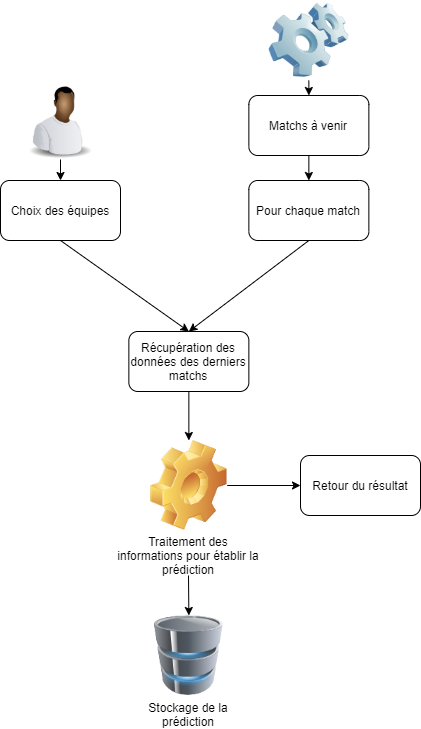
\includegraphics[height=18cm]{../img/schemaFonctionnement.png}
    \caption{Diagramme de fonctionnement}
    \label{fig:schemaFonctionnement}
\end{figure}

\newpage

\subsection{Description détaillée}

\subsubsection{Élaboration des prédictions}
\label{elaborationPredictionCDC}

La prédiction se crée en se basant sur les statistiques des matchs précédents de chacune des équipes. Un score offensif et défensive sera calculé pour chacun des équipes. Après comparaison des scores des deux équipes, l'application détermine le vainqueur (ou non, en cas d'égalité) de cette rencontre. 
 Les statistiques choisies pour le score offensif sont : 
\begin{itemize}
    \item Possession de balle
    \item Nombre d'attaques effectuées
    \item Nombre d'attaques dangereuses effectuées
    \item Nombre de tirs cadrés
    \item Nombre de tirs tentés
    \item Nombre de buts marqués
\end{itemize}

Les statistiques choisies pour le score défensif sont : 
\begin{itemize}
    \item Nombre de tacles
    \item Nombre de fautes
    \item Nombre de cartons jaunes
    \item Nombre d'arrêts
    \item Nombre de buts encaissés
\end{itemize}
De plus, elle utilise la forme du moment pour pouvoir effectuer son calcul. On entend par "forme du moment" si l'équipe est en série de victoires ou de défaites.
\subsection{Base de données}
\textbf{Initialement prévu :}

La base de données est là pour stocker les prédictions et avoir un historique sur ces dernières. Elle permet de montrer les prédictions précédentes faites par l'application à un instant T.

\textbf{Ajouté durant le projet :}

Cette dernière contient les matchs avec leurs statistiques\footnote{On stocke les matchs en base pour diminuer le nombre d'appels faits à l'API.}, ainsi que l'historique des appels faits à l'API (pour la fonctionnalité Head To Head)

\newpage

\subsection{API}

L'API possède plusieurs plans. J'ai réussi à avoir le plan "European" pour la durée de ce travail en expliquant la situation aux développeurs de l'API et ils m'ont permis d'avoir plus d'accès aux données dans l'API.

L'API que j'utilise pour avoir des données sur les matchs de football est APIFootball\footnote{\url{https://apifootball.com/}}. Les endpoints que j'utilise sont : 
\begin{itemize}
    \item Countries
    \begin{itemize}
        \item Permet de récupérer les pays. 
    \end{itemize}
    \item Competitions
    \begin{itemize}
        \item Permet de récupérer toutes les compétitions d'un pays en particulier
    \end{itemize}
    \item Teams
    \begin{itemize}
        \item Permet de récupérer toutes les équipes d'un championnat (ou compétitions)
    \end{itemize}
    \item Events
    \begin{itemize}
        \item Permet de connaître les matchs d'une date X à une date Y
    \end{itemize}
    \item Statistics
    \begin{itemize}
        \item Permet de récupérer les statistiques selon l'identifiant d'un match. Très utile pour élaborer une prédiction.
    \end{itemize}
    \item H2H 
    \begin{itemize}
        \item Permet de récupérer les derniers résultats entre une équipe A et une équipe B
    \end{itemize}
\end{itemize}

\subsection{Maquettes}
La page d'accueil du site permettra de voir le résultat des derniers matchs avec la prédiction qui a été faite par l'application. (voir fig. \ref{fig:accueil})

\begin{figure}[H]
    \centering
    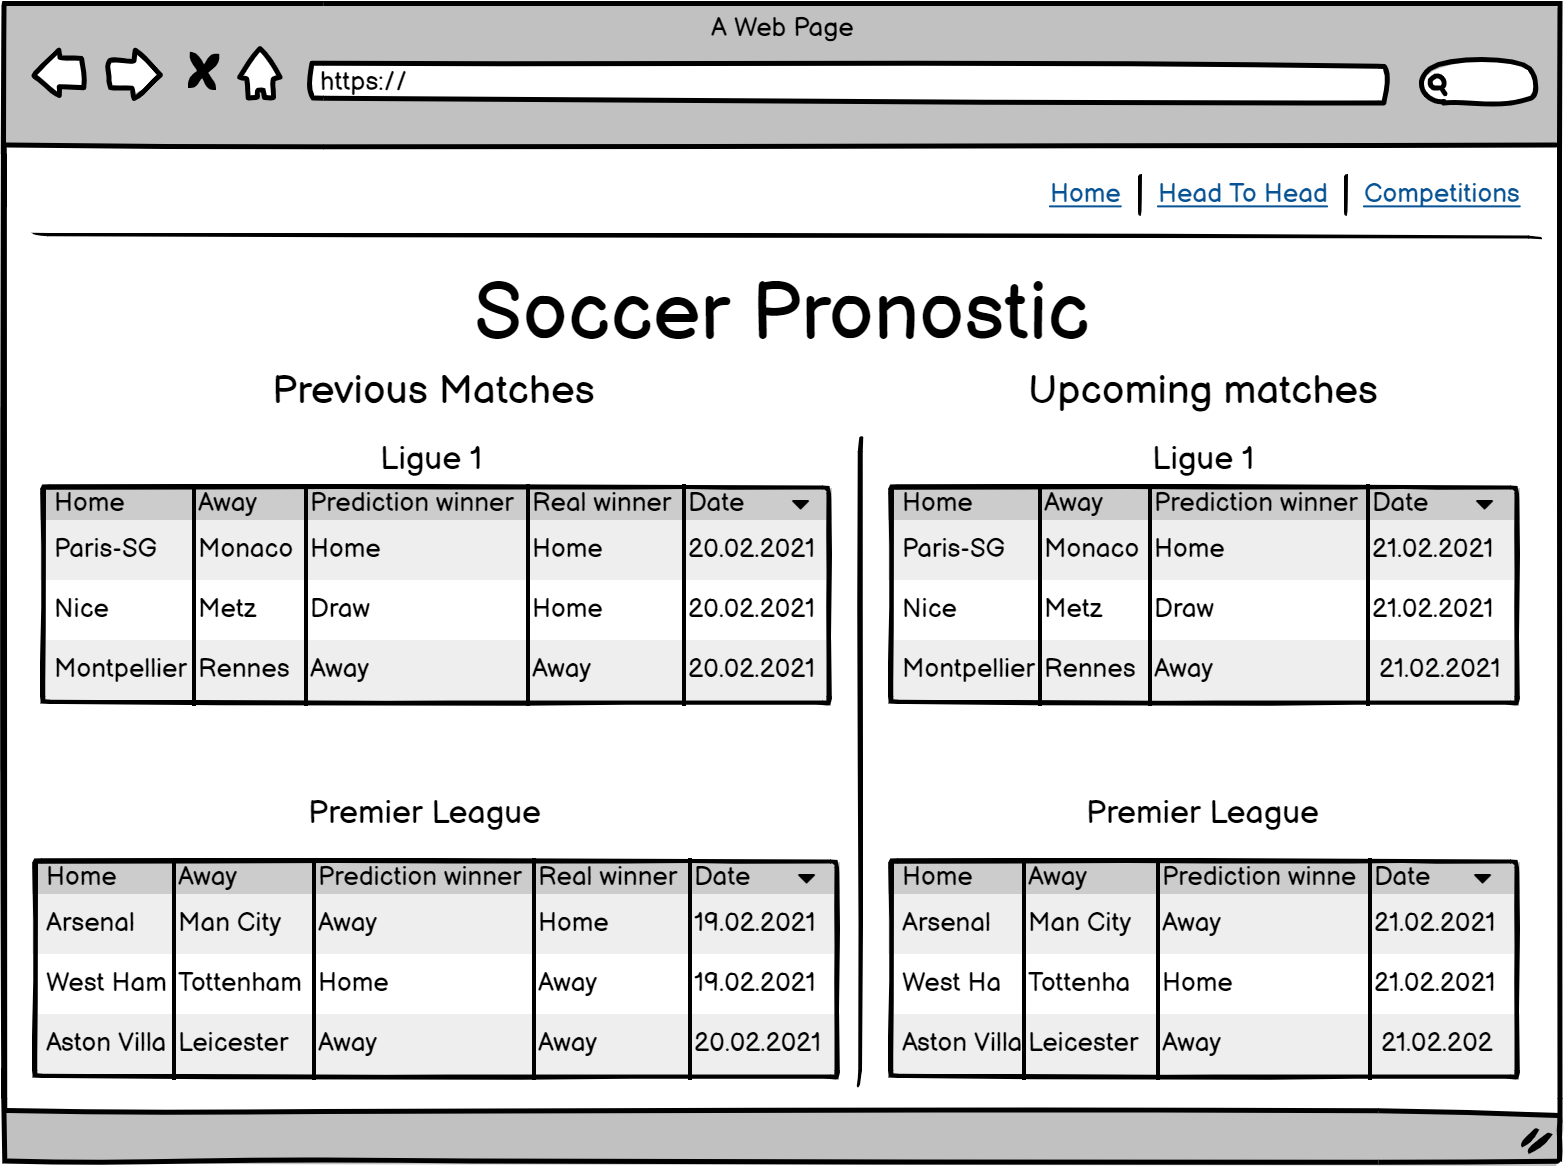
\includegraphics[width=13cm]{../img/maquetteAccueil.png}
    \caption{Accueil de l'application}
    \label{fig:accueil}
\end{figure}

\begin{figure}[H]
    \centering
    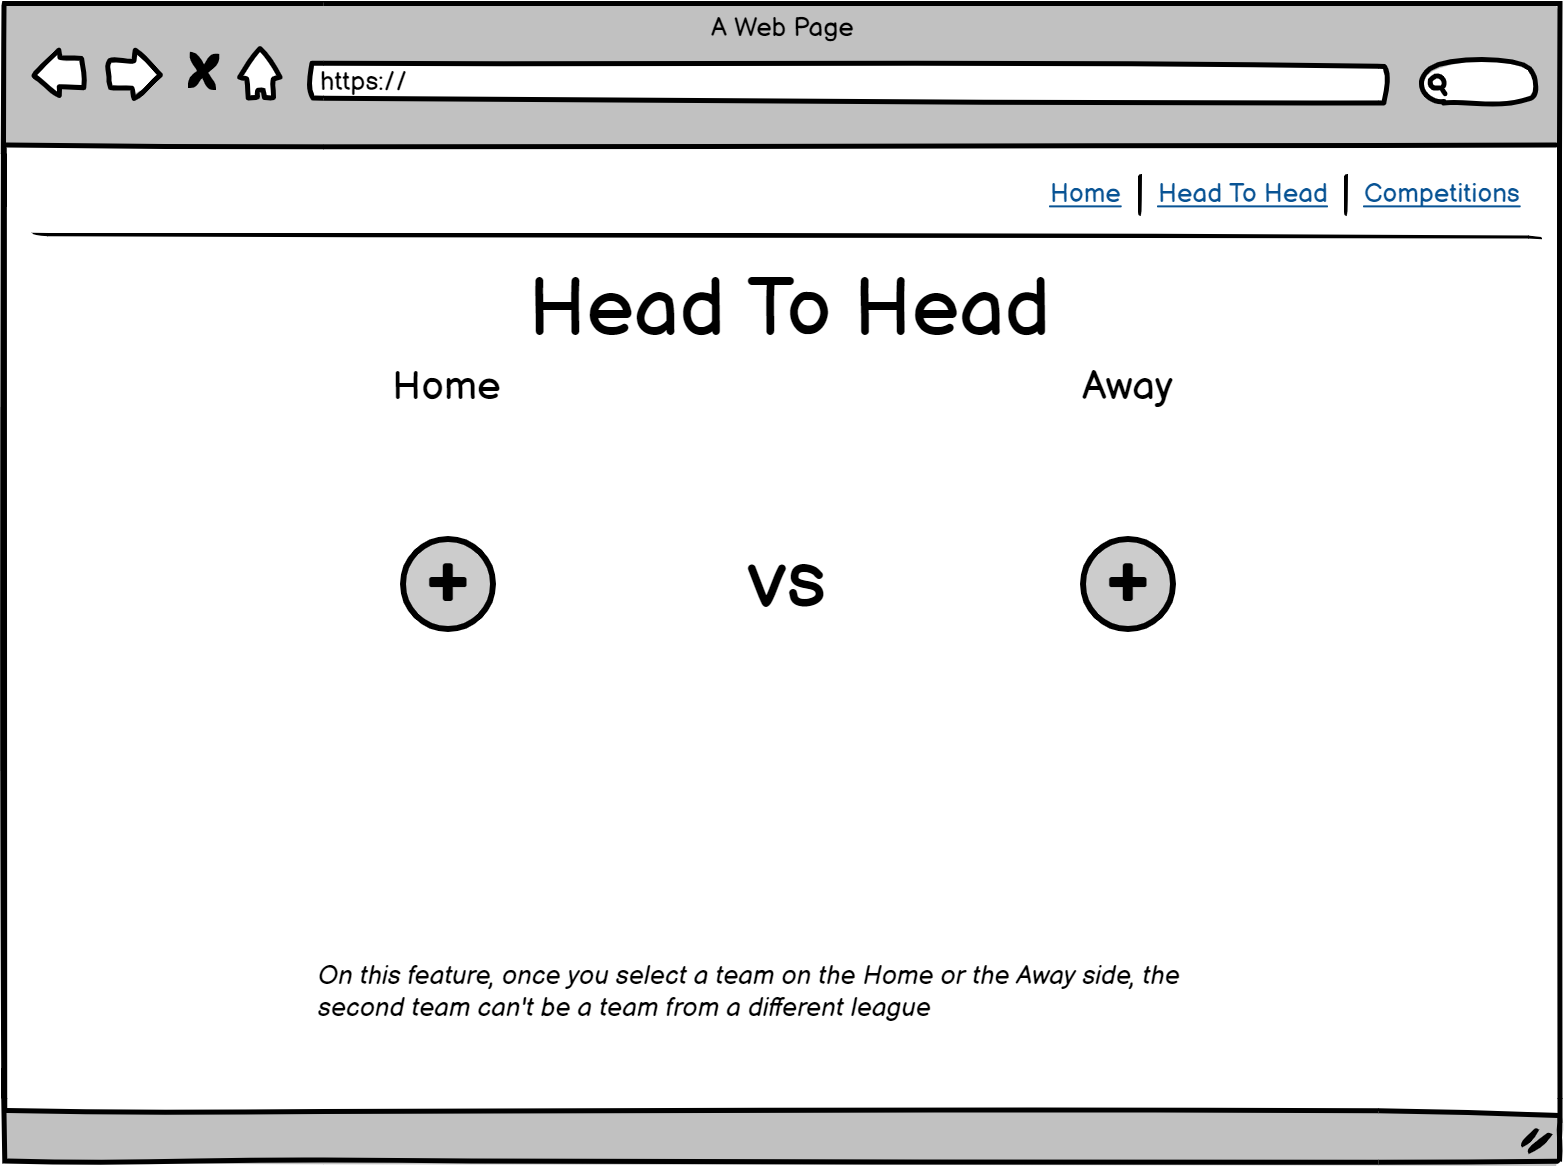
\includegraphics[width=13cm]{../img/maquetteH2H_1.png}
    \caption{Fonctionnalité Head to Head - Prédiction hypothétique}
    \label{fig:maquetteH2H_1}
\end{figure}

\begin{figure}[H]
    \centering
    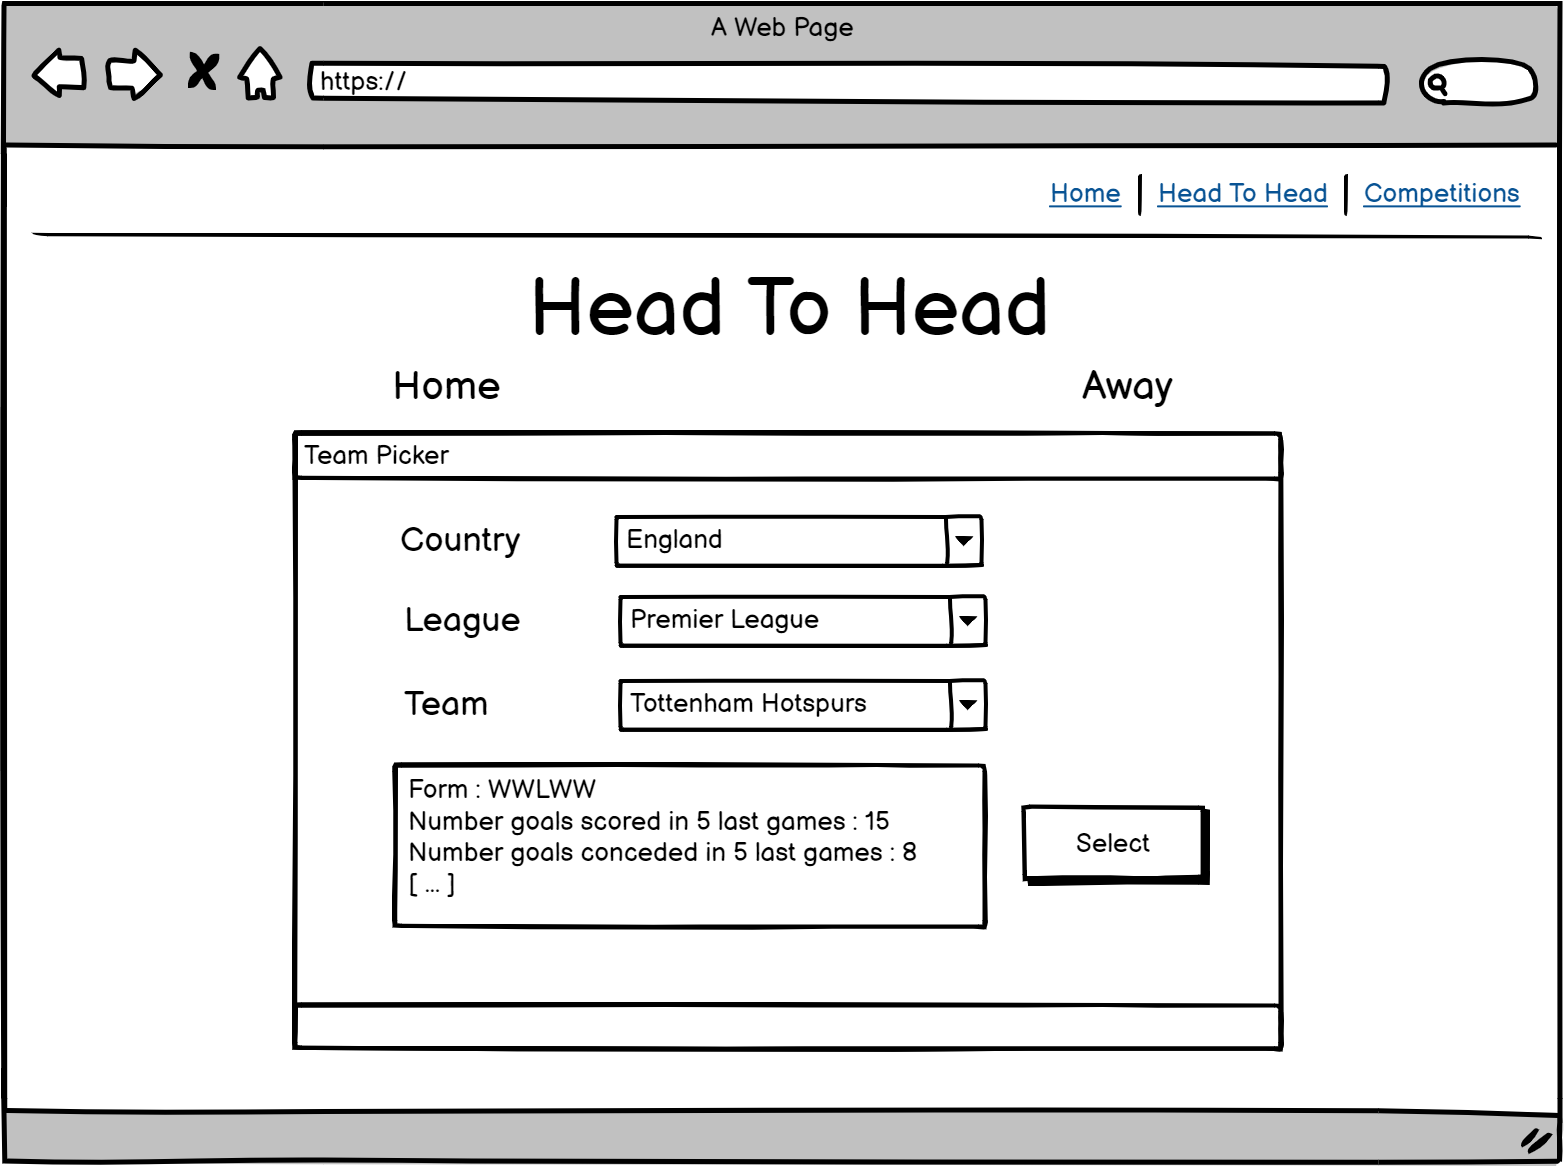
\includegraphics[width=13cm]{../img/maquetteH2H_2.png}
    \caption{Fonctionnalité Head to Head - Sélection}
    \label{fig:maquetteH2H_2}
\end{figure}

\begin{figure}[H]
    \centering
    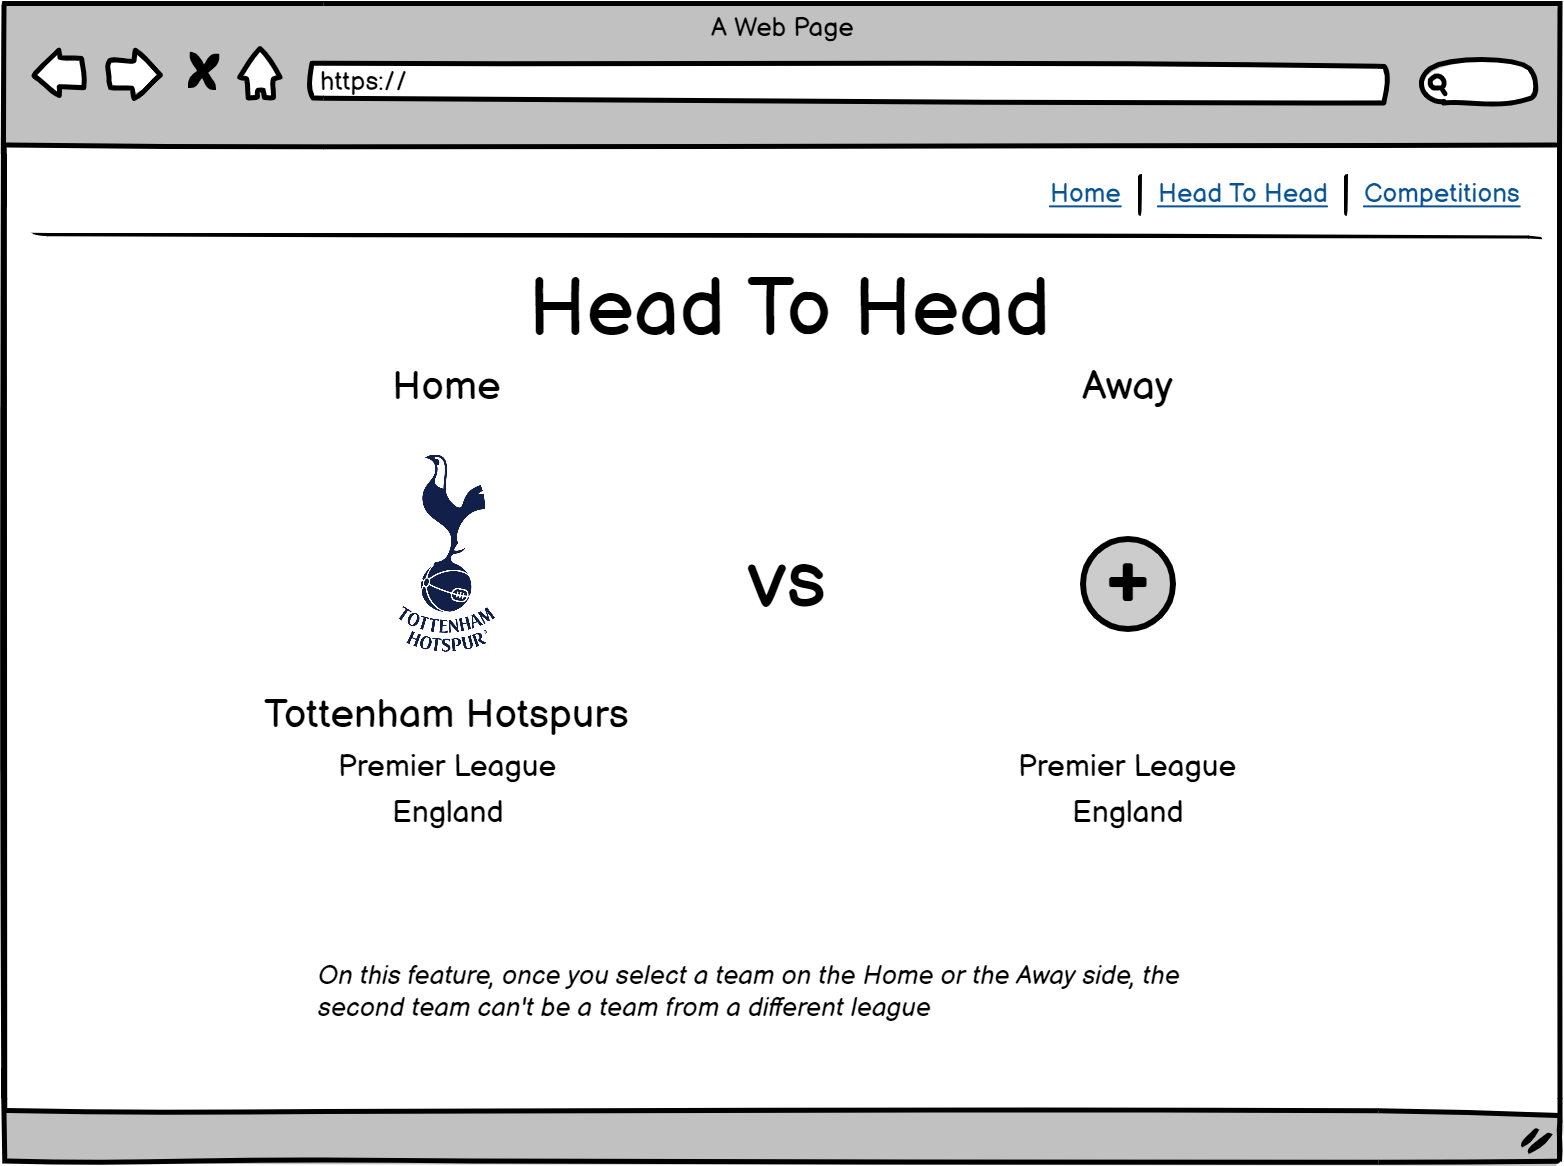
\includegraphics[width=13cm]{../img/maquetteH2H_3.png}
    \caption{Fonctionnalité Head to Head - Équipe sélectionnée}
    \label{fig:maquetteH2H_3}
\end{figure}

\begin{figure}[H]
    \centering
    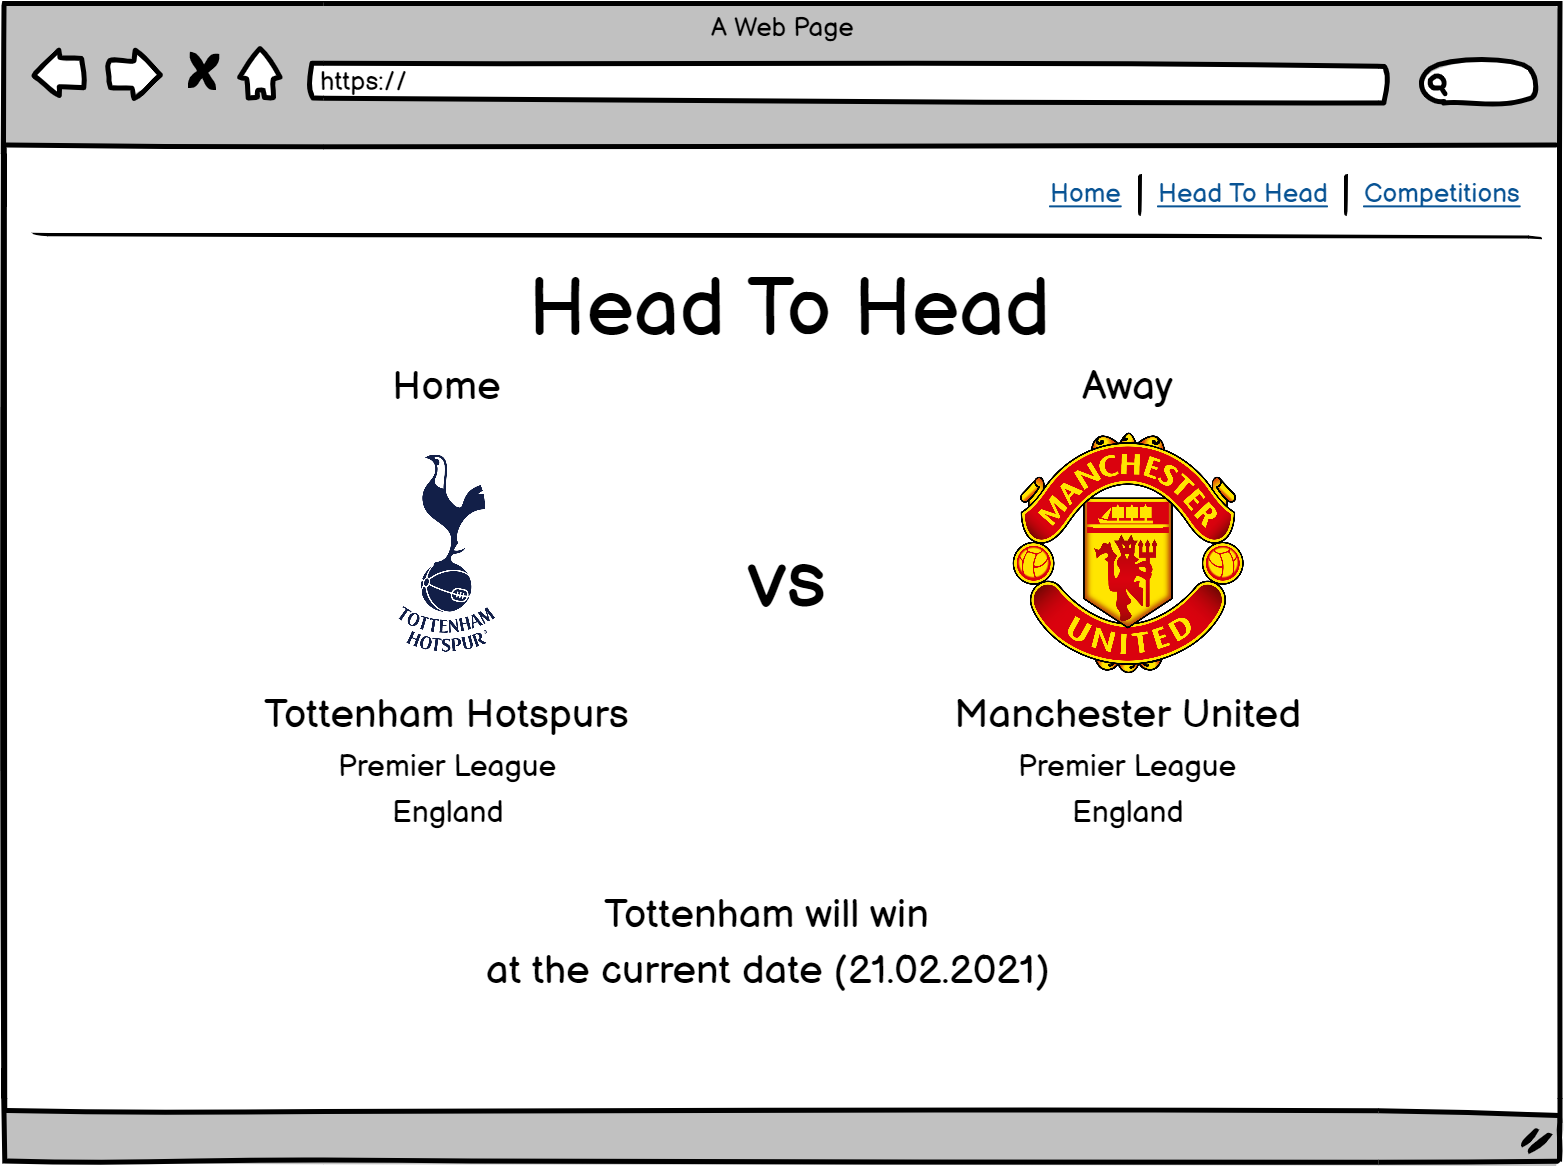
\includegraphics[width=13cm]{../img/maquetteH2H_4.png}
    \caption{Fonctionnalité Head to Head - Affichage de la prédiction}
    \label{fig:maquetteH2H_4}
\end{figure}

\begin{figure}[H]
    \centering
    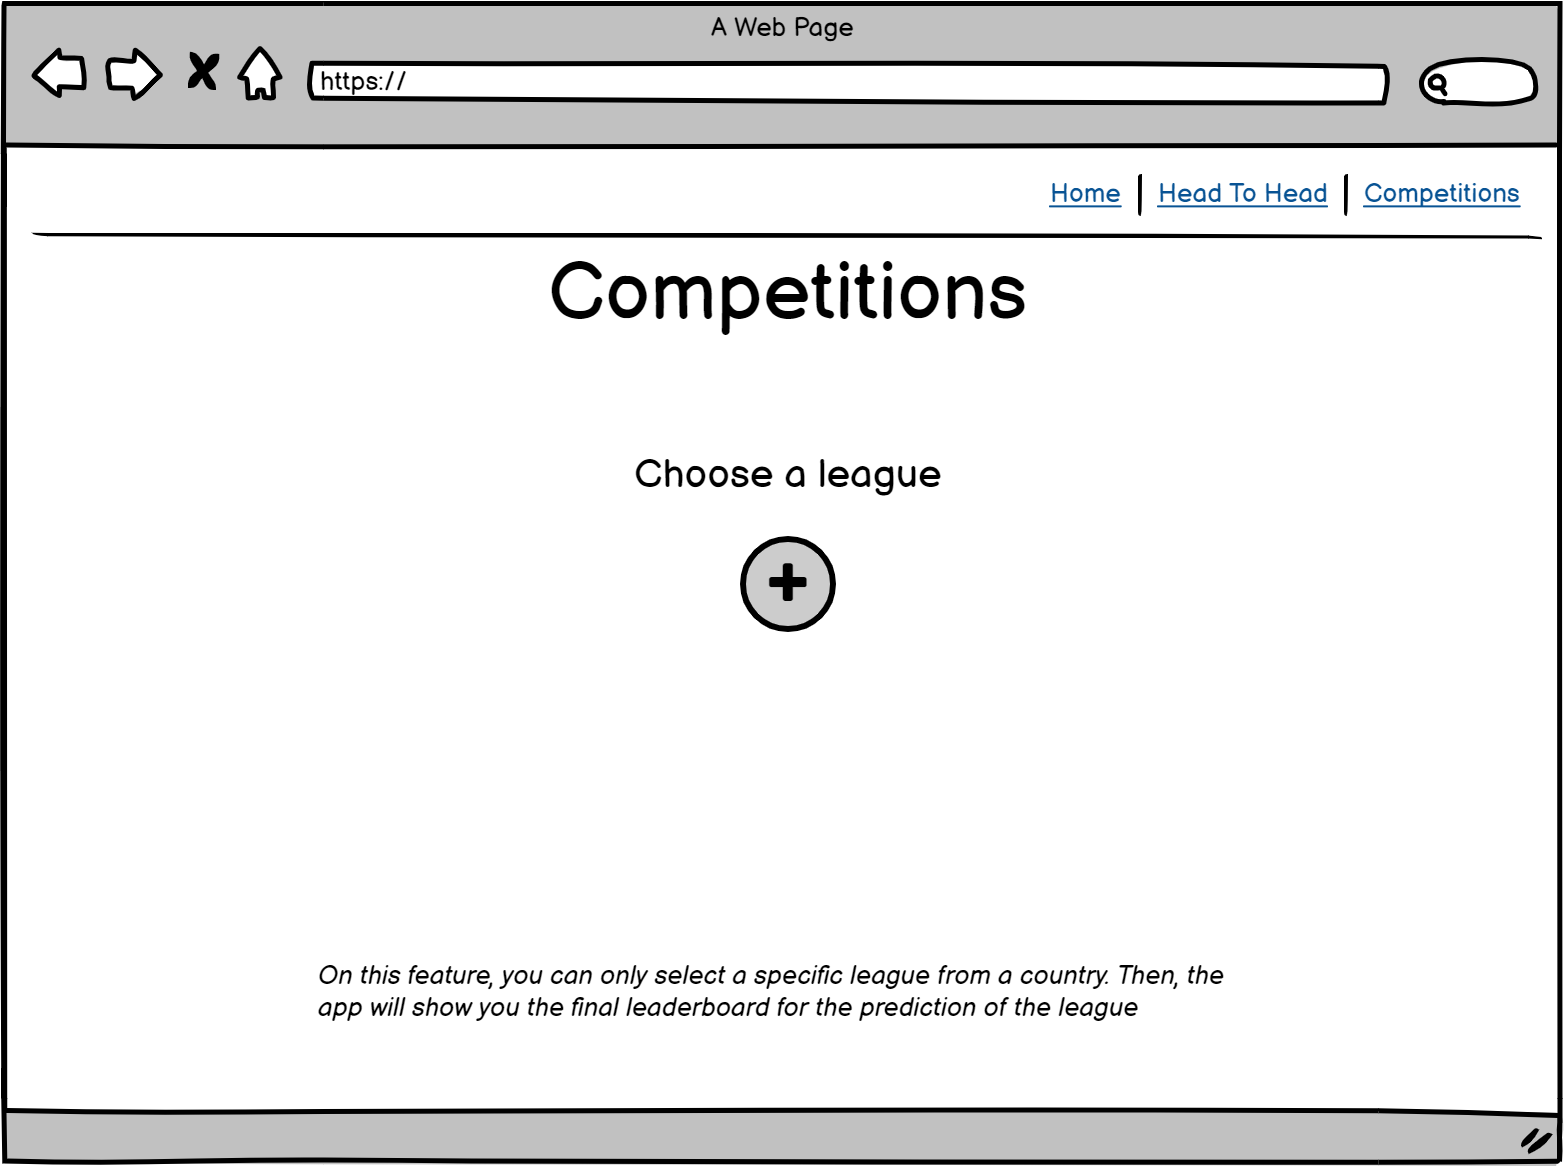
\includegraphics[width=13cm]{../img/maquetteCompetitions_1.png}
    \caption{Fonctionnalité Compétitions - Prédiction sur une compétition}
    \label{fig:maquetteCompetitions_1}
\end{figure}

\begin{figure}[H]
    \centering
    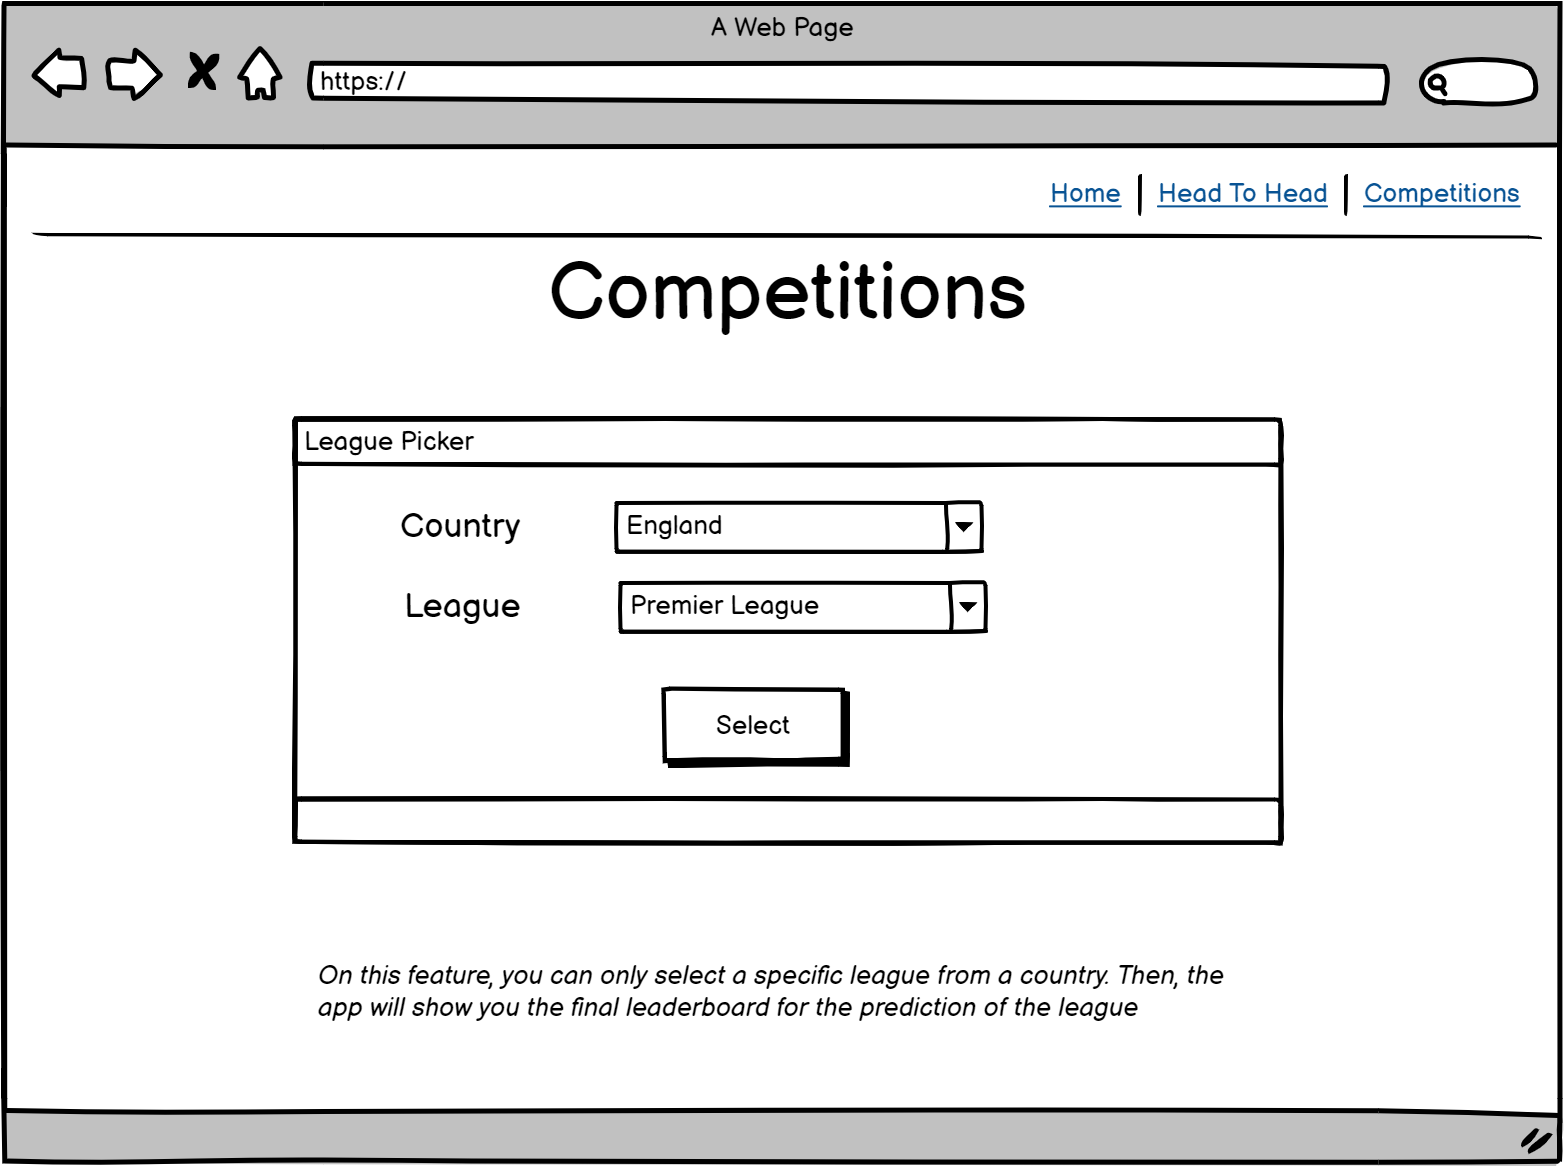
\includegraphics[width=13cm]{../img/maquetteCompetitions_2.png}
    \caption{Fonctionnalité Compétitions - Sélection}
    \label{fig:maquetteCompetitions_2}
\end{figure}

\begin{figure}[H]
    \centering
    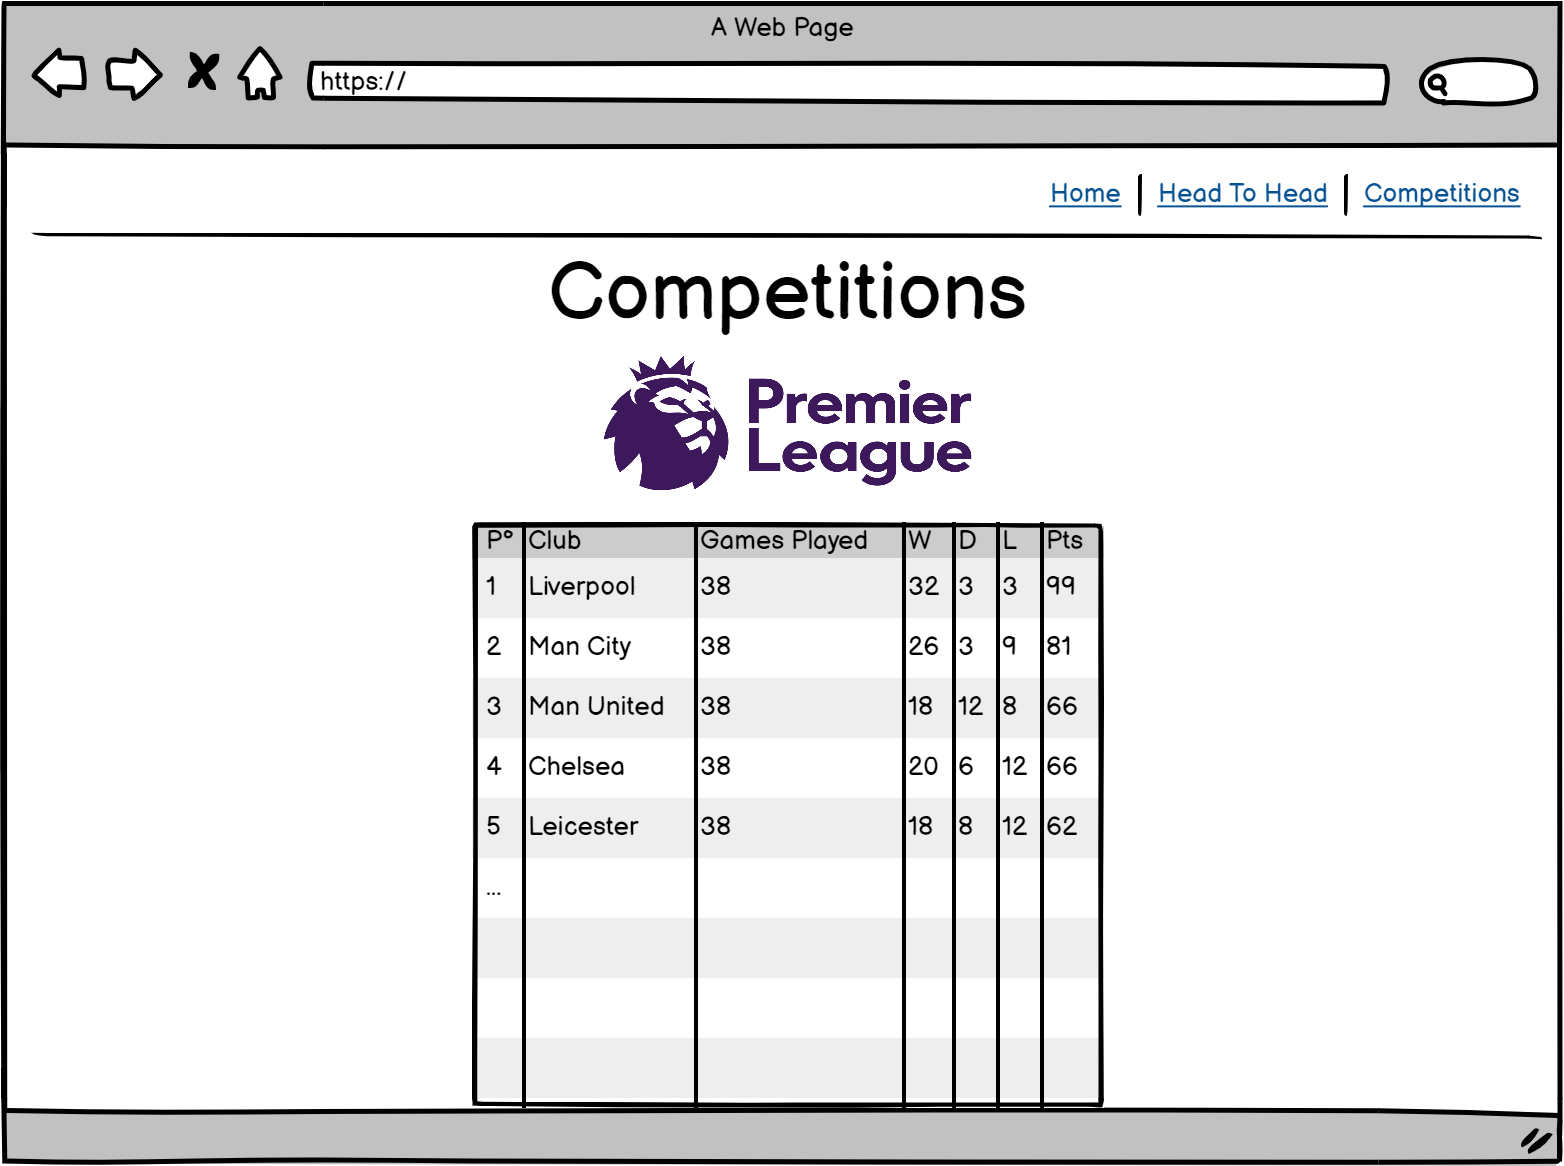
\includegraphics[width=13cm]{../img/maquetteCompetitions_3.png}
    \caption{Fonctionnalité Compétitions - Affichage de la prédiction}
    \label{fig:maquetteCompetitions_3}
\end{figure}

\begin{figure}[H]
    \centering
    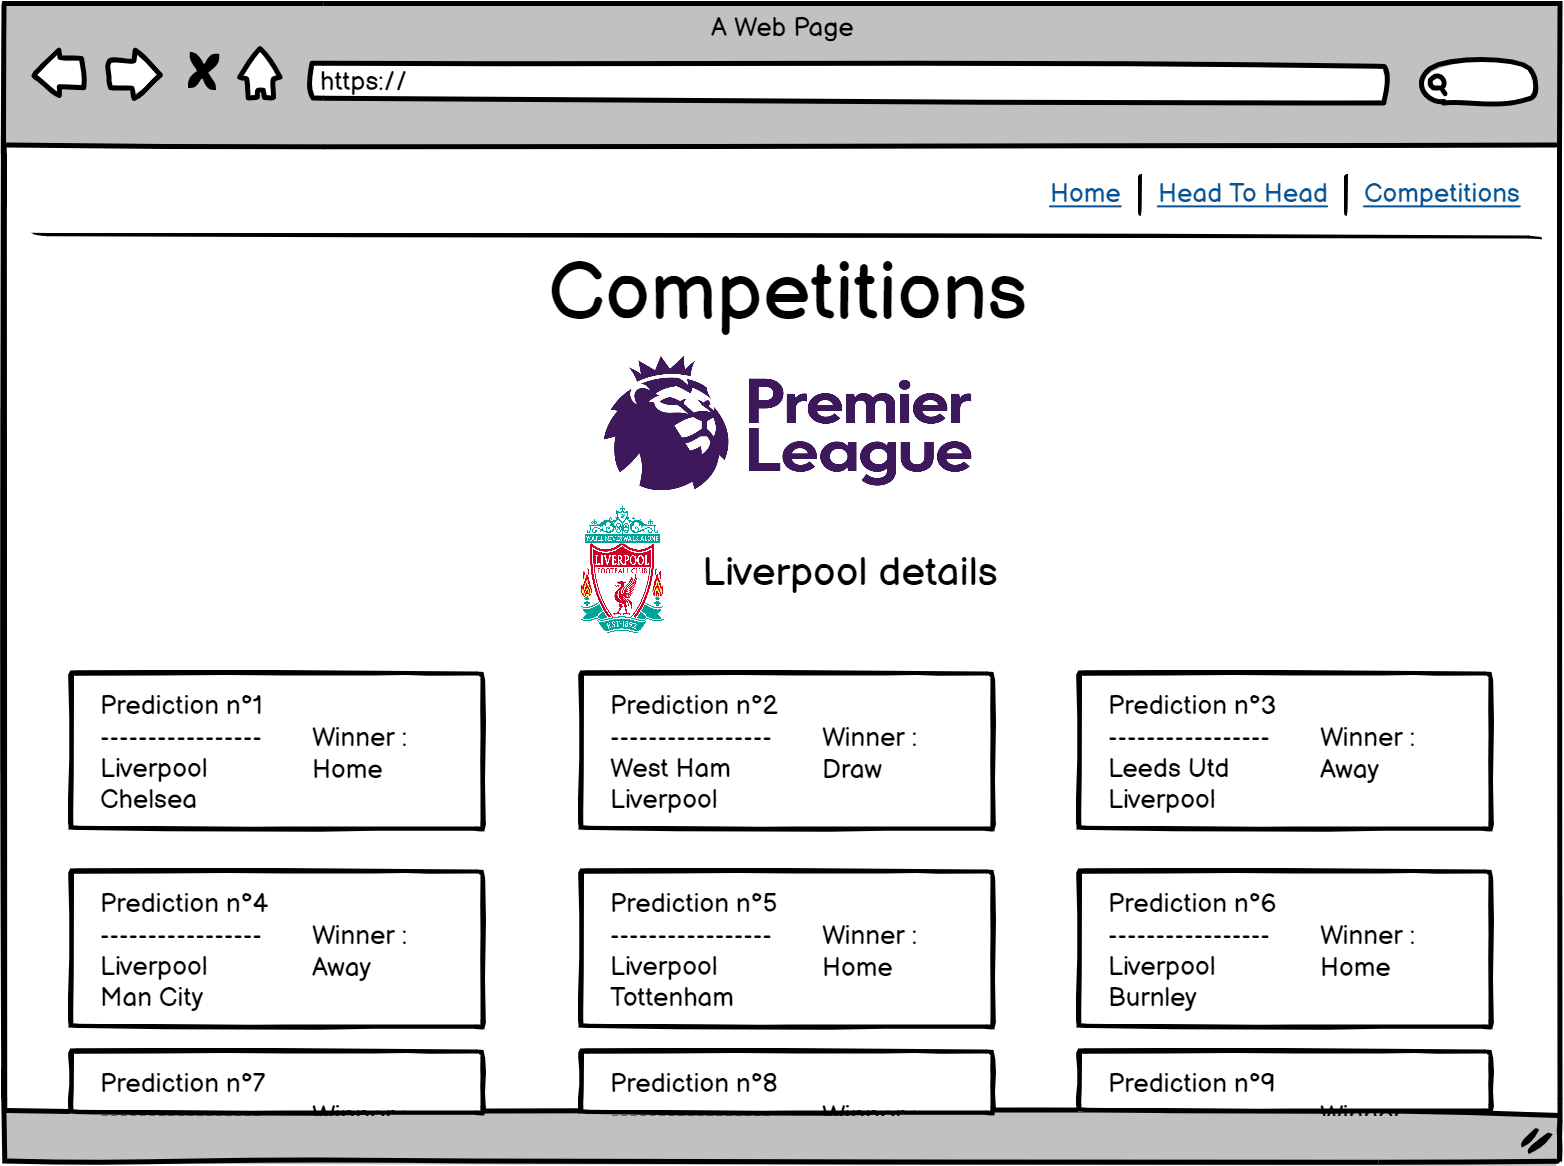
\includegraphics[width=13cm]{../img/maquetteCompetitions_4.png}
    \caption{Fonctionnalité Compétitions - Affichage détaillé}
    \label{fig:maquetteCompetitions_4}
\end{figure}

\subsection{User Stories}

\subsubsection{Utilisateur}

En tant qu’utilisateur, je souhaite pouvoir voir les prochains matchs qui vont se jouer et pouvoir avoir la prédiction faite par l’application. 

En tant qu’utilisateur, je souhaite voir les matchs qui se sont joués précédemment et d’avoir accès aux prédictions faites par l’application sur ces matchs-là, pour me faire une idée sur la fiabilité de l’application. 

En tant qu’utilisateur, je veux choisir deux équipes et voir le résultat de leur confrontation, car je veux une source pour m’aider à faire un choix sur un pari sportif. Cette fonctionnalité me permettrait d’avoir des résultats hypothétiques. 

En tant qu’utilisateur, lorsque je choisis les équipes pour effectuer une confrontation hypothétique, je souhaite pouvoir voir les statistiques actuelles de l’équipe que je choisis pour me faire une idée de sa forme actuelle. 

En tant qu’utilisateur, je veux pouvoir faire une prédiction sur un championnat entier et le programme sort une prédiction sur qui sera le vainqueur de ce championnat. 

En tant qu’utilisateur, je veux avoir un détail sur le parcours de chaque équipe dans le championnat. 

\subsubsection{Développeur}

En tant que développeur, je ne veux pas que l’utilisateur choisisse une équipe d’une autre compétition lorsqu’il effectue une confrontation hypothétique.

\subsection{Analyse SWOT}

\begin{table}[H]
    \centering
    \begin{tabular}{|l|l|}
    \hline
    \textbf{Forces}                                                                                                                                                        & \textbf{Faiblesses}                                                               \\ \hline
    \begin{tabular}[c]{@{}l@{}}Permet de simplifier le travail\\ d’analyse des pronostiqueurs\\ \\ Utilise plusieurs technologies\end{tabular}                             & \begin{tabular}[c]{@{}l@{}}Fiabilité et précision\\  des prédictions\end{tabular} \\ \hline
    \textbf{Opportunités}                                                                                                                                                  & \textbf{Menaces}                                                                  \\ \hline
    \begin{tabular}[c]{@{}l@{}}Peut s’améliorer au niveau des prédictions \\ (analyse de joueurs blessés, match important, \\ domicile, extérieur, huis clos)\end{tabular} & Dépendance à l’API                                                                \\ \hline
    \end{tabular}
    \caption{Analyse SWOT}
    \label{tab:SWOT}
\end{table}


\subsection{Livrables}
En termes de livrables pour ce projet, je dois rendre :
\begin{itemize}
    \item Code source
    \item Planning
    \item Documentation technique
    \item Logbook
    \item Résumé et Abstract
\end{itemize}

\newpage

\subsection{Dates importantes}

\begin{itemize}
    \item Lundi, 19 avril 2021 : Début du travail de diplôme
    \item Vendredi, 30 avril 2021 : Évaluation intermédiaire 1
    \item Vendredi, 14 mai 2021 : Rendu du rapport intermédiaire + poster + abstract (pour conseils par l’enseignant d’anglais)
    \item Jeudi, 20 mai 2021 après-midi, soirée poster : amis, famille, CFC, experts
    \begin{itemize}
        \item 14h00 : visite des classes de 1ère année (cf. SG)
        \item 16h30 : amis, famille, experts, enseignants Tech ES…
        \item 18h00 : fin de la soirée poster
    \end{itemize}	
    \item Lundi, 31 mai 2021 : Évaluation intermédiaire 3
    \item Vendredi, 11 juin 2021 : Rendu du travail avant 12h
    \item Jeudi, 17 juin 2021 : Défenses à blanc + harmonisation des notes
    \item Lundi, 21 juin 2021 / mardi 22 juin 2021 : Défenses des diplômes

\end{itemize}

\subsection{Contact}

{\underline{Étudiant :}}
\begin{itemize}
    \item David Paulino, \textbf{david.plnmr@eduge.ch}
\end{itemize}
 {\underline{Responsable du projet :}}
\begin{itemize}
    \item Antoine Schmid, \textbf{antoine.schmid@edu.ge.ch}
\end{itemize}

\newpage

\section{Charte graphique du projet}

Cette charte graphique sera utile pour avoir un respect des couleurs et des polices entre le poster et l'application.

Les couleurs sont très importantes dans une application. Chaque couleur a sa signification inconsciente. La couleur bleu est la plus populaire et elle symbolise la confiance et la fiabilité\footnote{\url{https://smart-origin.com/2018/03/08/choix-couleurs/} \url{https://99designs.fr/blog/conseils-design/signification-couleurs/}}.

J'ai utilisé Adobe Color\footnote{\url{https://color.adobe.com/fr/create}} pour trouver une nuance de bleu qui me convenait.

\definecolor{primary}{RGB}{76,97,237}
\definecolor{secondary}{RGB}{31,40,97}

\subsection{Couleur principale}
La couleur principale du projet et le \#4c61ed \fcolorbox{black}{primary}{\rule{0pt}{6pt}\rule{6pt}{0pt}}.

\subsection{Couleur secondaire}
La couleur secondaire du projet et le \#1f2861 \fcolorbox{black}{secondary}{\rule{0pt}{6pt}\rule{6pt}{0pt}}.

\subsection{Police de caractère principale}
La police principale du projet est \textbf{Poppins}.

\subsection{Police de caractère secondaire}
La police secondaire du projet est \textbf{Aleo}.

\newpage

\section{Football et son imprévisibilité}

Je tiens tout de même à en parler dans ce chapitre de mon rapport pour montrer l'imprévisibilité\footnote{Je vous redirige vers une vidéo de Le Monde qui explique cela - \url{https://www.youtube.com/watch?v=L1V7w4TAof0}} du football en général. 

C'est un fait qui est très peu connu. En effet, le football est définitivement le sport d'équipes le plus imprévisible et le plus dur à prédire. 

Commençons par analyser les vainqueurs de la compétition la plus prestigieuse, la Coupe du monde. Les 5 derniers pays ayant gagné la compétition sont tous différents (France, Allemagne, Espagne, Italie, Brésil). Uniquement deux nations ont réussi à garder leur titre l'édition suivante (Italie en 1934-38, et le Brésil 1958-62). 

Comparons ces informations avec les mêmes compétitions mais dans les autres sports. La Coupe du monde de handball a vu 3 champions différents sur les 5 dernières éditions (Le Danemark 2019-21, la France 2011, 2015 et 2017, Espagne en 2013). Pour la Coupe du monde de basketball, c'est 4 équipes différentes depuis l'édition de 1967 (Russie, Yougoslavie, États-Unis et Espagne). 

Les surprises sont bien plus fréquentes dans ce sport. On peut parler de certains cas comme celui de Leicester City lors de la saison 2015-16 de Premier League qui fut sacré champion alors qu'avant la saison, les bookmakers avait établi la cote pour cette situation à 5000 contre 1, soit la cote maximale. On pourrait parler aussi de l'arrivée en demi-finale de l'Ajax Amsterdam après avoir vaincu le Real Madrid et la Juventus de Cristiano Ronaldo. Ou encore la victoire du FC Porto lors de la Ligue des Champions en 2003.

Cette imprévisibilité s'explique par le nombre de buts plus faible au football que dans les autres sports cités précédemment. Cela amène à des écarts au score moins élevés qui déboulent sur des potentielles erreurs individuelles qui coûtent cher. Il est simple pour une équipe non favorite de marquer un but, d'avoir l'avantage au score et d'opter pour une stratégie défensive pour gagner le match. Tandis qu'au basketball, ce genre de stratégie ne peut tout simplement pas fonctionner.

Maintenant, dans sa globalité, on peut quand même remarquer qu'il y a des choses récurrentes qui arrive et qu'elle ne sont pas anodines :
\begin{itemize}
    \item Le PSG domine le football français
    \item Le Real Madrid et le FC Barcelone se disputent chaque année le championnat espagnol
    \item Le Bayern maîtrise totalement la ligue allemande
    \item La ligue anglaise voit son haut du classement géré par le Big Four\footnote{\url{https://fr.wikipedia.org/wiki/Big_Four_(football)}} (ou Big Six désormais)
\end{itemize}
Ces faits peuvent nous laisser dire qu'il y a tout de même moyen de prédire certains résultats. Cependant, ces prédictions ne seront pas sans failles dû aux nombreux rebondissement qui peuvent apparaître lors d'un match. 

\section{Analyse de l'existant}

\subsection{Kickoff.ai}
\begin{figure}[H]
    \centering
    
\includegraphics{../img/kickoffai.png}
    \caption{Logo de Kickoff.ai}
    \label{fig:logoKickoffAI}
\end{figure}

Kickoff.ai\footnote{\url{http://kickoff.ai/}} est une application de prédiction sur des rencontres de football. Elle a été créé par deux étudiant en doctorat en "Machine Learning" à l'École Polytechnique de Lausanne. L'application fonctionne avec des inférences\footnote{\url{https://fr.wikipedia.org/wiki/Inférence}}. Ce sont des analyses de probabilités grâce aux statistiques des précédents matchs. 

\subsection{Matchs prochainement joués}

\begin{figure}[H]
    \centering
    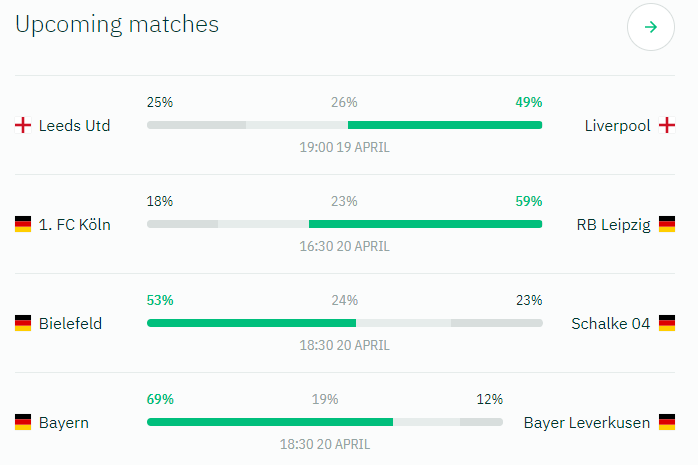
\includegraphics[width=12cm]{../img/upcomingMatches.png}
    \caption{Kickoff.ai - Match prochainement joués}
    \label{fig:kickoff.ai_upcomingmatches}
\end{figure}

Sur la figure \ref{fig:kickoff.ai_upcomingmatches}, l'application retourne le pourcentage de chance qu'une victoire d'une équipe arrive.

\subsection{Matchs précédemment joués}

\begin{figure}[H]
    \centering
    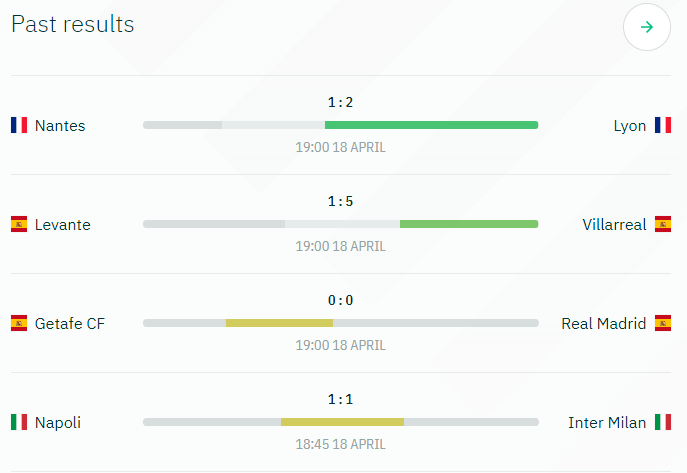
\includegraphics[width=12cm]{../img/pastResults.png}
    \caption{Kickoff.ai - Matchs précédemment joués}
    \label{fig:kickoff.ai_pastresults}
\end{figure}

L'application affiche le résultat du match précédent et le pourcentage de chance qu'elle avait prévu pour que ce cas arrive. (voir fig. \ref{fig:kickoff.ai_pastresults})

\subsection{Différences avec notre application}

\textbf{Kickoff.ai} ne permet pas de faire une prédiction sur une compétition entière ou de permettre à l'utilisateur de faire une prédiction hypothétique. Cependant, l'application est beaucoup plus poussée techniquement, ce qui rend, en théorie, leur application plus fiable au niveau des prédictions.

\section{Organisation}

\subsection{Gestion de projet}

Pour planifier les tâches de mon projet, j'ai décidé d'utiliser Trello\footnote{\url{https://trello.com/}}. Cette application web permet de créer des tâches de les organiser librement, les ajouter à des catégories que l'on aura créé, etc. Toutes ces possibilités rend l'outil très pratique pour la gestion de projet. Cela nous évite de perdre du temps à chercher les tâches que l'on doit réaliser lors d'un projet. 

\subsection{Format de la documentation}

Étant à l'aise avec \LaTeX, j'ai décidé de créer ma documentation en utilisant cet outil. En effet, l'an dernier, j'ai découvert cet outil qui est très différent des outils de bureautiques classiques. \LaTeX{} permet de se focaliser sur le contenu de notre document plutôt que sur la forme. Cela permet de travailler efficacement et de ne pas perdre de temps sur la mise en page de notre documentation. L'outil permet aussi d'intégrer des paquets communautaires. Ces paquets peuvent nous permettre d'avoir du versionning automatique sur notre document ou encore d'insérer du code source. 

J'avais commencé à rédiger la documentation avec Overleaf\footnote{\url{https://www.overleaf.com/}}, qui est un éditeur et compilateur \LaTeX{} en ligne. Cela facilite la transportabilité et cela évite d'installer un compilateur localement. Cependant, j'ai rencontré un soucis avec cet outil. Ce dernier intègre un timeout d'une minute\footnote{Le timeout est de 4 minutes si on upgrade notre compte.} lors de la compilation d'un projet \LaTeX{}. 

C'est pourquoi, j'ai du utiliser un compilateur \LaTeX{} en local et ne plus profiter des avantages d'Overleaf. J'utilise l'extension VSCode "LaTeX Workshop" qui permet de compiler un fichier \LaTeX{} depuis Visual Studio Code. Il utilise le compilateur "latexmk" par défaut mais on a aussi la possibilité d'utiliser "pdflatex". Il permet ensuite d'afficher le PDF converti dans un tab de VSCode.

\subsection{Système de sauvegarde et de versionning}

Pour garder mon projet et pour gérer ses versions, j'ai utilisé différentes types de sauvegardes.

Tout d'abord, j'ai utilisé Git. Cet outil permet de sauvegarder et de faire du versionning sur le code source du projet. Il permet aussi au responsable de mon projet de voir l'avancement du projet. Ce dépôt est hébergé sur GitHub\footnote{\url{https://github.com/}}. J'ai choisi cet hébergeur essentiellement pour la fiabilité de son service et pour sa simplicité d'utilisation. 

Ensuite, j'ai fait un backup hebdomadairement de mon repértoire de travail sur ma clé USB personnelle pour éviter d'avoir une totale dépendance à GitHub. 

\section{Technologies utilisées}

\subsection{Python}
Python\footnote{\url{https://www.python.org/}} est un langage de programmation qui favorise la programmation orientée objet. Sa première version date de 1991 et il a été mis à jour le 4 avril 2021 sous la version 3.9.4. Le langage a comme particularité d'être multiplateforme ce qui permet d'être exécuté sous n'importe quel OS.

\subsubsection{Utilisation}
J'ai choisi de développer mon projet en Python car c'est le langage que je maîtrise le plus. J'ai pu faire beaucoup de projets en Python au sein de l'école, ce qui m'a permis d'acquérir de l'expérience avec le langage. De plus, le langage permet de faire des requêtes à des API très rapidement.

\subsubsection{Librairies utilisées}

\textbf{Dotenv}\footnote{\url{https://pypi.org/project/python-dotenv/}}
La librairie Dotenv est une librairie qui permet d'avoir des variables d'environnement, ce qui est très utile pour éviter de stocker des données sensibles, telles que des mots de passe de base de données ou des tokens d'API. Pour pouvoir récupérer les variables d'environnement, il faut importer \texttt{os} dans notre fichier pour accéder au variable d'environnement du système.

\textbf{Logging}\footnote{\url{https://docs.python.org/3/library/logging.html}}
La librairie Logging me permet de garder une trace sur les actions effectuées par l'application. 

\textbf{MySQL.Connector}\footnote{\url{https://dev.mysql.com/doc/connector-python/en/}}
La librairie MySQL.Connector permet à l'application de se connecter à une base de données et de pouvoir faire différentes requêtes sur cette dernière. 

\textbf{Requests}\footnote{\url{https://pypi.org/project/requests/}}
La librairie Requests permet de faire des requêtes HTTP de manière très élégante et épurée. C'est avec cette librairie que je fais des requêtes à ma source de données. 

\textbf{JSON}\footnote{\url{https://docs.python.org/3/library/json.html}}
Cette librairie permet de sérialiser et désérialier des objets JSON. 

\textbf{Multiprocessing}\footnote{\url{https://docs.python.org/3/library/multiprocessing.html}}
Multiprocessing permet de paralléliser des tâches pour réduire le temps d'exécution d'algorithmes qui prennent du temps.

\textbf{Python Flask}\footnote{\url{https://flask.palletsprojects.com/en/1.1.x/}}
Flask est un framework web écrit en Python. C'est le framework web le plus populaire, ce qui fait qu'il est mis à jour régulièrement. Flask me sert de vue pour mon application. Le framework permet de créer des routes de manière très efficace.

\textbf{Asyncio}\footnote{\url{https://pypi.org/project/asyncio/}}
Asyncio est une librairie qui permet de faire de l'asynchrone en Python en utilisant les mots clés \texttt{async} et \texttt{await}.

\textbf{Aiohttp}\footnote{\url{https://docs.aiohttp.org/en/stable/}}
Aiohttp est une librairie qui, contrairement à \textbf{Requests}, permet de faire de l'asynchrone sur des requêtes HTTP. Ces requêtes sont moins élégantes que la librairie \textbf{Requests}.

\subsubsection{Architecture}
\begin{figure}[htp]
    \centering
    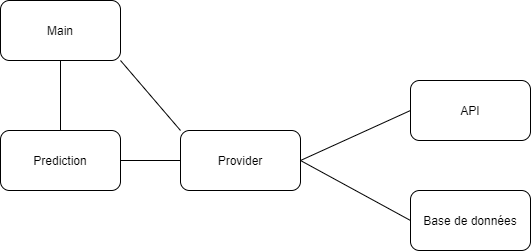
\includegraphics[width=15cm]{../img/architectureClasse.png}
    \caption{Architecture du projet}
    \label{fig:architectureClasse}
\end{figure}

Sur la figure \ref{fig:architectureClasse}, le \texttt{Provider} sert d'intermédiaire pour la vue et pour la classe \texttt{Prediction}. Dans ce \texttt{Provider}, on peut y trouver des méthodes qui permet de mettre les données de l'API dans le bon format pour la classe qui fera les pronostics, pour récupérer les prédictions stockées en base pour la vue, etc.

\subsubsection{Arborescence de fichiers}

Une capture d'écran de l'arborescence de fichiers est disponible (voir fig. \ref{fig:schemaDB}). 

\begin{itemize}
    \item \textbf{Dossier /doc} Ce repértoire contient les fichiers et les outils nécessaire à l'élaboration de la documentation du projet (notamment le source \LaTeX{}).
    \item \textbf{Dossier /lib} Ce dossier contient la façade, la classe pour la communication avec la base de données, le provider et la classe pour établir une prédiciton
    \item \textbf{Dossier /log} Contient les logs de l'application. Ce répertoire et le fichier qui est dedans sont créé lors du premier lancement de l'application. Ils sont aussi inclus dans le \texttt{.gitignore} pour éviter de potentiels conflits git.
    \item \textbf{Dossier /static} Contient les fichiers statiques de l'application (CSS, JS et différentes images\footnote{Mis à part les images des équipes qui sont stockés sur le serveur de l'API} et favicons).
    \item \textbf{Dossier /templates} Contient les fichiers de templating pour l'affichage de la vue (HTML avec le templating de Jinja2).
    \item \textbf{Dossier /tests} Contient les fichiers de tests pour le backend et le frontend de l'application.
    \item \textbf{Dossier /venv} Contient tous les fichiers liés à l'environnement virtuel Python. Ce répertoire est inclu dans le \texttt{.gitignore} car il contient toutes les dépendances de l'application et qu'il est très volumineux.
    \item \textbf{Fichier .env} Contient les variables d'environnement locale du projet
    \item \textbf{Fichier app.py} Contient les routes de l'application web et toutes le code pour formatter les données pour l'affichage.
    \item \textbf{Fichier requirements.txt} Contient toutes les dépendances de l'application avec leurs versions. Ce fichier permet d'installer de manière efficace les dépendances de l'application en utilisant \texttt{pip3}.
\end{itemize}

\begin{figure}[htp]
    \centering
    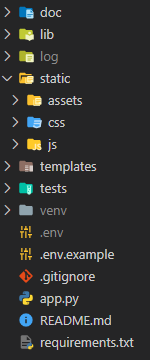
\includegraphics[height=18em]{../img/arborescenceFichier.png}
    \caption{Arborescence de fichier du projet}
    \label{fig:arborescenceFichier}
\end{figure}

\subsection{MySQL}

MySQL\footnote{\url{https://www.mysql.com/}} est un SGBD (système de gestion de base de données) relationnelles. Il permet de stocker des données dans une base et de pouvoir les manipuler. Sa première version date de 1994 et il a été mis à jour le 20 avril 2021 sous la version 8.0.24. 

\subsubsection{Utilisation}
J'ai choisi ce système car c'est celui avec lequel j'ai le plus d'expérience. Sa popularité est un atout. Cela permet de faciliter la résolution de certains problèmes que l'on peut rencontrer lors de requêtes.

\subsubsection{Architecture}

\begin{figure}[htp]
    \centering
    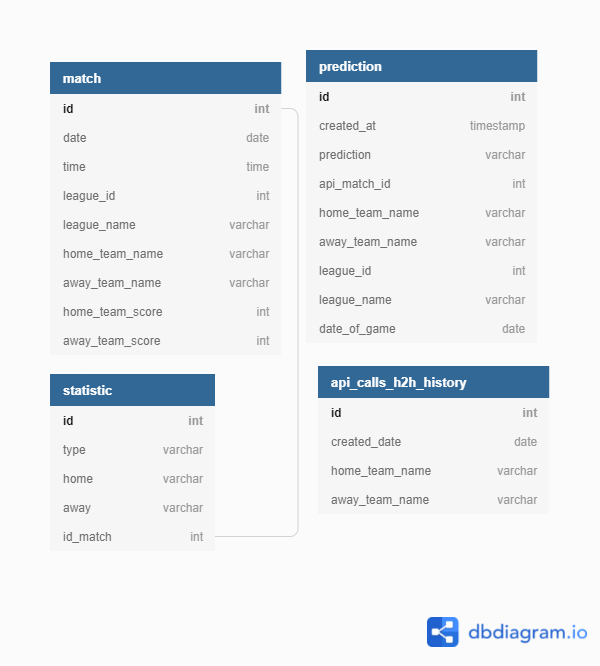
\includegraphics[width=21.5em]{../img/schemaBDDv2.png}
    \caption{Schéma de la base de données du projet}
    \label{fig:schemaDB}
\end{figure}

\newpage

\subsection{Documentation}

\subsubsection{Paquets \LaTeX{} utilisés}

\noindent\textbf{Lstlisting}
Ce paquet permet d'insérer des codes sources dans notre PDF. Il y a la possibilité d'ajouter des paramètres pour afficher les lignes, pour spécifier le langage ou pour changer le style.

\noindent\textbf{VHistory}
Ce paquet apporte du versioning automatique à \LaTeX. Il gère automatiquement le numéro de version et les auteurs des versions.

\subsubsection{Doxygen}
Doxygen\footnote{\url{https://www.doxygen.nl/index.html}} est un générateur de documentation libre de droit qui permet de produire une documentation à partir du code source d'un logiciel. Il peut exporter la documentation en HTML et/ou \LaTeX{}. Pour ce faire, il faut utiliser la syntaxe du langage dans lequel on écrit le code source. Doxygen va alors analyser tout le code pour produire une documentation générée automatiquement. Pour Python, la syntaxe est \newline 
\texttt{"""} \newline
\texttt{Comments. } \newline
\texttt{"""} \newline

\subsection{Outil d'automatisation de tests}
\label{outilAutomatisationTest}

Katalon Recorder\footnote{\url{https://chrome.google.com/webstore/detail/katalon-recorder-selenium/ljdobmomdgdljniojadhoplhkpialdid}} est l'extension de navigateur de Katalon Studio. Katalon Studio est un outil d'automatisation de tests. Il peut automatiser les tests pour des interfaces webs, des APIs, des applications mobiles ou encore des applications de bureau.

\subsubsection{Utilisation}

Dans ce projet, j'ai utilisé Katalon Recorder\footnote{Le tutoriel officiel pour utiliser Katalon Recorder : \url{https://www.youtube.com/watch?v=sgzFkQ-0Ta8&t=151s}} pour pouvoir tester l'interface web de mon application. Cela me permet d'automatiser un jeu de tests qui vérifie que les erreurs apparaissent bien lorsque des données incorrectes sont transmises et aussi lorsque les données sont correctes et que l'application retourne un bon résultat.

\subsubsection{Katalon TestOps}

En utilisant Katalon Recorder, on peut créer un projet de visualisation sur la réussites des tests. C'est ce que permet de faire Katalon TestOps. Cette interface web est liée à notre compte Katalon et lorsque l'on clique sur \textbf{Report} dans Katalon Recorder (voir fig. \ref{fig:reportKatalonRecorder}), nous avons la possibilité d'upload les résultats des tests que l'on a joué sur le visualiseur.
\begin{figure}[htp]
    \centering
    
\includegraphics[width=5em]{../img/reportKatalonRecorder.png}
    \caption{Bouton Report Katalon Recorder}
    \label{fig:reportKatalonRecorder}
\end{figure}

Le visualiseur permet de savoir si les tests se sont bien passés, s'ils ont eu des erreurs (voir fig. \ref{fig:dashboardTestOps}). On voit aussi combien de temps ont pris les tests à être utilisé. Cet outil est très intéressant lorsque l'on travaille à plusieurs sur un projet.
Le graphique sur la figure \ref{fig:dashboardTestOps} est le graphique qui montre le temps écoulé lors du lancement des tests.

\begin{figure}[htp]
    \centering
    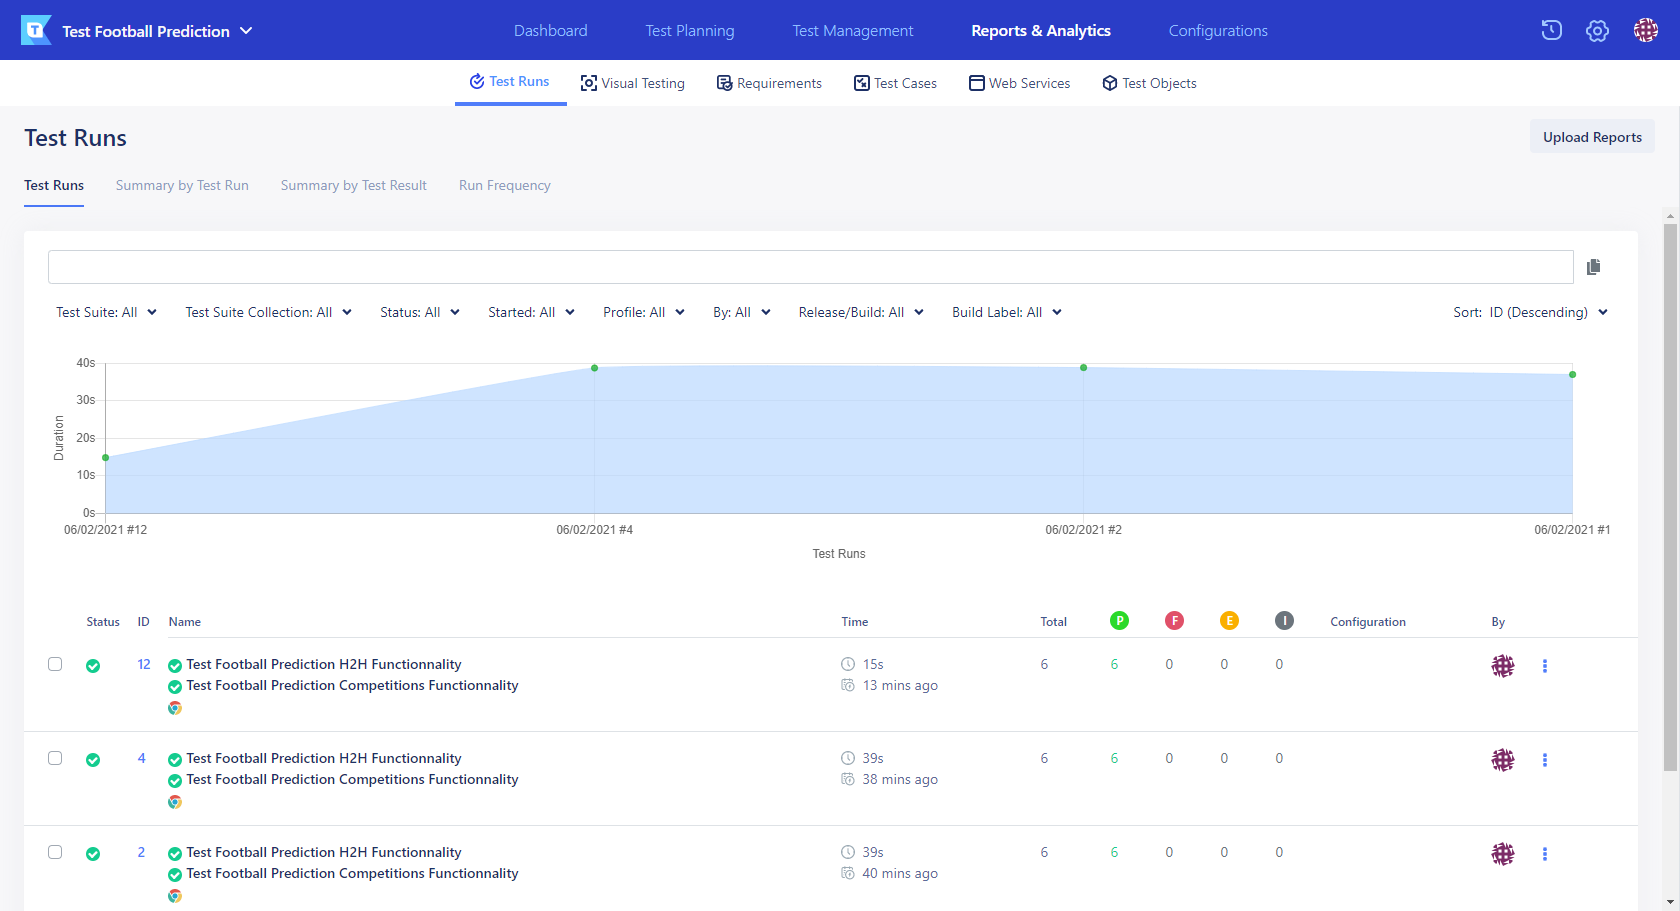
\includegraphics[width=30em]{../img/dashboardTestOps.png}
    \caption{Dashboard Katalon TestOps}
    \label{fig:dashboardTestOps}
\end{figure}

\newpage

\subsection{Bootstrap}

Bootstrap\footnote{\url{https://getbootstrap.com/}} est une collection d'outils qui permet de simplifier la création du design de sites et d'applications web. Des templates d'application sont aussi disponibles pour une structure déjà faite. Bootstrap permet de gagner du temps sur le design de son site.

\subsubsection{Utilisation}

J'ai cherché un template Bootstrap pour avoir une structure déjà faite et j'ai trouvé un template qui me plaisait qui se nomme Freelancer\footnote{\url{https://startbootstrap.com/theme/freelancer}}. J'ai ensuite changé les couleurs pour ne pas garder les couleurs par défaut et utiliser les couleurs de ma charte graphique. 

\newpage

\section{Recherche de solutions}

\subsection{Élaboration de prédictions}

L'idéal pour l'application serait de pouvoir donner deux équipes différentes pour ensuite ressortir le vainqueur du match. L'application récupère les résultats ainsi que les statistiques des derniers matchs de chacune des équipes et elle les analyse pour ensuite établir un score final qui nous permettra de déterminer le vainqueur.


\subsubsection{Niveau des différents championnats}
\label{niveauDifferentChampionnats}
Au niveau des restrictions de l'application, cette dernière ne peut qu'établir une prédiction entre deux équipes du même championnat. En effet, il n'y a aucun moyen de déterminer si un championnat d'un pays est plus fort qu'un autre et donc qu'une équipe d'un championnat est meilleure qu'une autre. 

Prenons un cas concret avec comme exemple, un match entre Anderlecht (BEL) et le FC Bayern (ALL). Dans le cas ou le Bayern est dans une série de défaites et que l'Anderlecht dans une série de victoires, l'application sortira probablement l'équipe d'Anderlecht comme vainqueur de cet affrontement, ce qui a très peu de chance d'arriver. 
On pourrait envisager de prendre le classement du championnat national de l'Allemagne et de la Belgique et de dire que le premier du classement de Belgique a le même niveau que le premier allemand, mais ce n'est pas envisageable car ces équipes n'ont pas le même niveau.  

Une autre solution qui est plus envisageable mais qui a toujours un problème : le coefficient de clubs des associations de l'UEFA\footnote{\url{https://fr.uefa.com/memberassociations/uefarankings/country/\#/yr/2021}}. Ce coefficient est utilisé pour déterminer le nombre de places disponibles dans un championnat pour accéder aux compétitions de clubs de l'UEFA. Par exemple, le championnat d'Angleterre est celui qui a le plus de places disponibles (voir fig. \ref{fig:coeffClubsAssoc}).

\begin{figure}[htp]
    \centering
    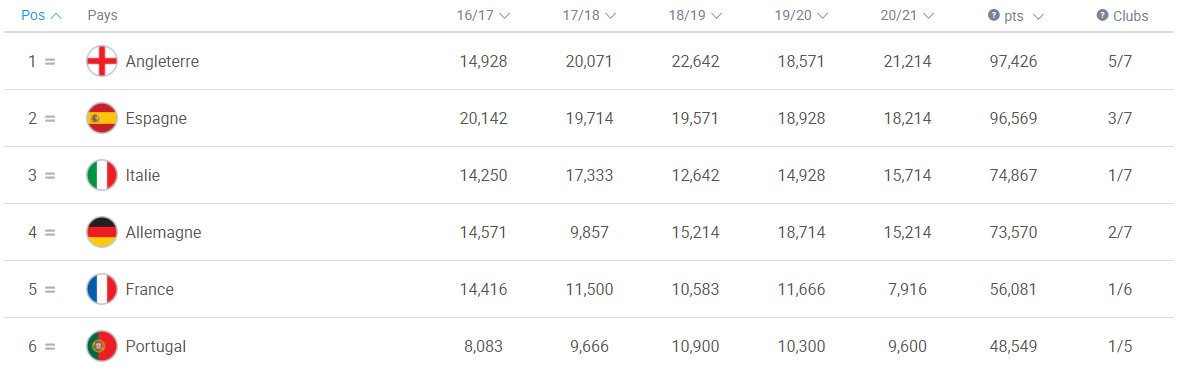
\includegraphics[width=16cm]{../img/coeffClubAssoc.png}
    \caption{UEFA - Coefficient de clubs des associations}
    \label{fig:coeffClubsAssoc}
\end{figure}

Tout d'abord, on peut se dire que c'est la solution miracle, mais il faut analyser un peu plus en profondeur cette solution.
%On va comparer la figure \ref{fig:coeffClubsAssoc} avec le coefficient des clubs qui est un autre indice de l'UEFA\footnote{\url{https://fr.uefa.com/memberassociations/uefarankings/club/#/yr/2021}}.

\begin{figure}[htp]
    \centering
    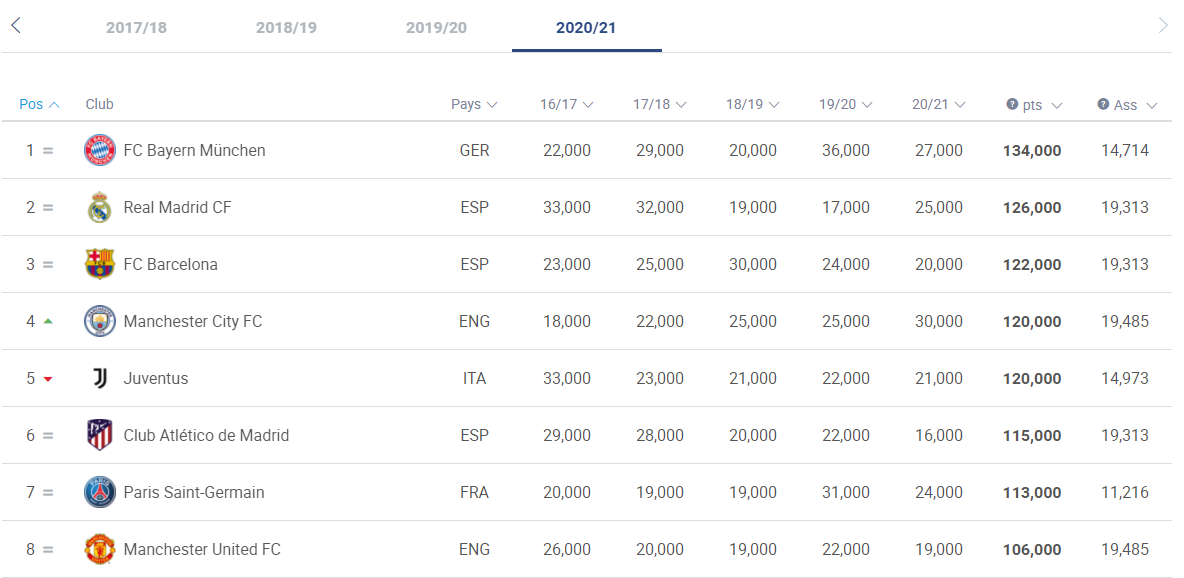
\includegraphics[width=16cm]{../img/coeffClubs.png}
    \caption{UEFA - Coefficient des clubs}
    \label{fig:coeffClubs}
\end{figure}

Comme on peut le voir sur la figure \ref{fig:coeffClubsAssoc}, l'Angleterre est le pays le plus haut du classement, ce qui signifie qu'il possède le plus de places pour les compétitions européennes. On pourrait en déduire aussi que c'est le meilleur championnat et donc que les équipes sont meilleures en Angleterre qu'ailleurs. Cependant, observons maintenant la figure \ref{fig:coeffClubs}. On peut voir que le Bayern de Munich est premier dans le classement des coefficient des clubs et que l'équipe anglaise la plus haute est Manchester City. On comprend donc que le Bayern, équipe allemande, a un meilleur indice UEFA que Manchester City.

En clair, ces classements ne peuvent pas être utilisé pour déterminer le niveau actuel des différentes équipes. Ces coefficients sont calculés sur la base des résultats des cinq dernières saisons\footnote{\url{https://fr.uefa.com/memberassociations/uefarankings/country/about/}}\footnote{\url{https://fr.uefa.com/memberassociations/uefarankings/club/about/}}, ce qui explique le classement de l'Inter dans ce tableau (voir fig. \ref{fig:classementInterUEFA}).  Pourtant l'Inter est actuellement la première équipe d'Italie devant la Juventus de Turin (5ème au classement de l'UEFA) qui est 4ème en Serie A (voir fig. \ref{fig:classementSerieA}).

\begin{figure}[htp]
    \centering
    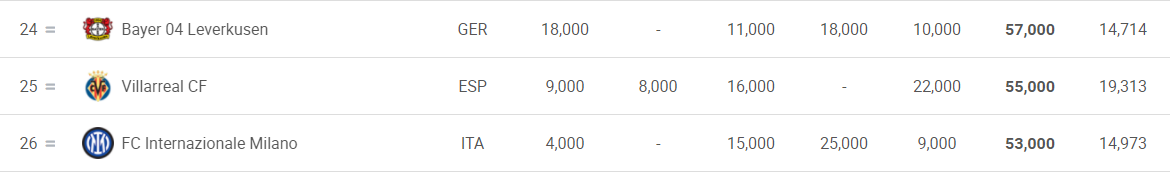
\includegraphics[width=16cm]{../img/classementInterUEFA.png}
    \caption{UEFA - Position Inter}
    \label{fig:classementInterUEFA}
\end{figure}

\begin{figure}[htp]
    \centering
    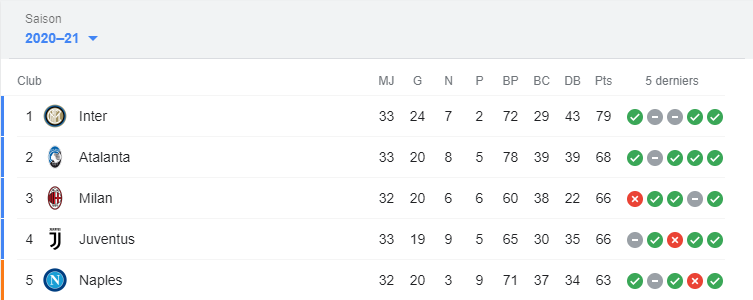
\includegraphics[width=16cm]{../img/classementSerieA.png}
    \caption{Serie A - Classement championnat}
    \label{fig:classementSerieA}
\end{figure}

Le choix que j'ai donc fait est d'uniquement prédire un match entre deux équipes du même championnat car ces deux équipes joueront forcément contre les mêmes équipes et c'est ce qui nous permet de déterminer qu'une équipe est meilleure qu'une autre.

\subsubsection{Récupération des matchs et de leurs statistiques}
\label{recupMatchStats}

Pour élaborer une prédiction dans mon projet, je me base sur les matchs précédents et sur leurs statistiques. Il va donc bien me falloir une source de données pour récupérer les informations de ces matchs. Dans mon cas, je vais utiliser une API et ma base de données (j'expliquerai dans le point \ref{test_pourcent_reussite} l'utilité de ma base de données)

Pour la communication avec l'API que j'utilise, M. Schmid m'a conseillé d'appliquer le design pattern \texttt{Façade}\footnote{\url{https://refactoring.guru/fr/design-patterns/facade}}. Ce design pattern a comme principe de créer une interface simple vers un système complexe. Dans ce projet, le système complexe est l'API. Cette interface est aussi extensible facilement. Cela permet l'ajout d'un nouvel appel à un endpoint de manière facilitée. 

Le travail principal du Provider (voir fig. \ref{fig:architectureClasse}) est de mettre les données de l'API ou de la base de données dans le bon format pour la classe \texttt{Prediction}.
Pour récupérer les matchs et les statistiques précédentes de chaque équipe, j'utilise l'endpoint \texttt{H2H} (Head To Head). On donne le nom de deux équipes en paramètre et l'API nous retourne les matchs récents de chacune des deux équipes \textbf{ainsi} que les dernières confrontations entre les équipes. 
Comme on peut l'apercevoir sur le listing \ref{apercuJSONH2H}, nous avons donné "Chelsea" et "Arsenal" comme paramètre de l'endpoint et on reçoit trois tableaux.

Ensuite, grâce au endpoint \texttt{Statistics}, je récupère les statistiques de chacun des matchs. Cependant, j'ai remarqué que tout les matchs de l'API n'ont pas toutes les statistiques dont j'ai besoin pour élaborer une prédiction . (voir point \ref{elaborationPredictionCDC}) J'ai du vérifié que chacun des matchs aient toutes les statistiques et si le match n'a pas toutes ces statistiques, je ne le prendrais pas en compte pour établir ma prédiction.

En effet, si je choisissais de faire une prédiction avec des données en moins, cela impliquerait un manque de fiabilité sur le pronostic. 

Cependant, il y a tout de même un risque sur la fiabilité de la prédiction en "jetant" les matchs qui manquent de statistiques. Effectivement, si sur 80\% des matchs d'une équipe manquent de statistiques, cela peut influencer drastiquement le pronostic fait par l'application. (voir fig \ref{fig:explicationStatsManquante}) Comme je n'ai pas trouvé de solution pour palier ce potentiel risque, j'ai décidé d'accepter cette éventualité qui créera un manque de fiabilité sur certaine prédiction.

Dans l'exemple de la figure \ref{fig:explicationStatsManquante}, disons que nous avons 4 victoires et 1 défaite pour le Sporting Portugal, ce qui est une forme très correcte pour une équipe. Son adversaire est le FC Porto et ces derniers ont 3 égalités, 1 victoire et 1 défaite. L'application a de grandes chances de dire que le Sporting sera le grand vainqueur de cette prédiction. Cependant, toutes les statistiques requises pour établir cette prédiction sont présentes dans les matchs récents du FC Porto mais malheureusement ce n'est pas le cas pour le Sporting Portugal, où les 4 victoires ont des statistiques qui manquent (donc les matchs ne seront pas pris en compte pour la prédiction). Dans ce cas là, l'application prédira potentiellement une victoire du FC Porto. Alors que par rapport aux résultats précédents de chacune des équipes, le Sporting Portugal se serait imposer dans cette prédiction.

\begin{figure}[H]
    \centering
    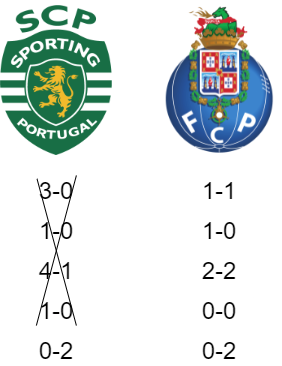
\includegraphics[height=10cm]{../img/explicationStatsManquante.png}
    \caption{Explication sur le manque de fiabilité probable sur les prédictions}
    \label{fig:explicationStatsManquante}
\end{figure}

\begin{lstlisting}[language=json, firstnumber=1, caption=Aperçu du JSON de l'endpoint H2H, captionpos=b, label=apercuJSONH2H]
[
 {
   "firstTeam_VS_secondTeam": [
  {
    "match_id": "218349",
    "country_id": "165",
    "country_name": "Europe",
    "league_id": "590",
    "league_name": "Europa League",
    "match_date": "2019-05-29",
    "match_status": "Finished",
    "match_time": "21:00",
    "match_hometeam_id": "2616",
    "match_hometeam_name": "Chelsea",
    "match_hometeam_score": "4 ",
    "match_awayteam_id": "2617",
    "match_awayteam_name": "Arsenal",
    "match_awayteam_score": " 1",
    "match_hometeam_halftime_score": "0",
    "match_awayteam_halftime_score": "0",
    "match_live": "0"
  },
 .....
   ],
   "firstTeam_lastResults": [
  {
    "match_id": "218349",
    "country_id": "165",
    .....
  },
  
 .....
   ],
   "secondTeam_lastResults": [
  {
    "match_id": "218349",
    "country_id": "165",
    .....
  },
 .....
]
\end{lstlisting}

\begin{lstlisting}[language=json, firstnumber=1, caption=Aperçu du JSON de l'endpoint Statistics, captionpos=b, label=apercuJSONStats]
{
    "24562": {
        "statistics": [
        {
            "type": "Ball Possession",
            "home": "60%",
            "away": "40%"
        },
        {
            "type": "Goal Attempts",
            "home": "18",
            "away": "10"
        },
        {
            "type": "Shots on Goal",
            "home": "6",
            "away": "5"
        },
        {
            "type": "Shots off Goal",
            "home": "5",
            "away": "1"
        },
        {
            "type": "Blocked Shots",
            "home": "7",
            "away": "4"
        },
        {
            "type": "Free Kicks",
            "home": "15",
            "away": "11"
        },
        {
            "type": "Corner Kicks",
            "home": "4",
            "away": "2"
        },
        {
            "type": "Offsides",
            "home": "2",
            "away": "1"
        },
        {
            "type": "Goalkeeper Saves",
            "home": "3",
            "away": "5"
        },
        {
            "type": "Fouls",
            "home": "10",
            "away": "14"
        },
        {
            "type": "Yellow Cards",
            "home": "2",
            "away": "1"
        }
        ]
    }
}
\end{lstlisting}

\subsubsection{Choix des championnats disponibles}

On a vu que d'évaluer le niveau des différents championnats est très complexe. Maintenant, on va parler du choix des championnats qui seront disponibles dans l'application.

Tout d'abord, le choix de ne pas prendre les championnats des équipes nationales (Euro, Coupe du monde, Coupe d'Afrique des Nations, etc.) est important à argumenter selon moi.
Pourquoi ai-je choisi de prendre uniquement prendre les championnats spécifiques à chaque pays ? 
Il y a deux explications  :
\begin{itemize}
    \item Le fréquence des matchs annuels
    \item Le renouvellement des joueurs de l'équipe nationale (sélectionneur)
\end{itemize}

La fréquence de matchs annuels pour les équipes nationales est très bas. Le Portugal a joué 6 matchs en 2020, 8 matchs en 2019. La France en a joué 6 en 2020 et 11 en 2019. L'Allemagne en a joué 6 en 2020 et 10 en 2019. On voit bien que le nombre de matchs par année est très faible. De plus, ces matchs sont des matchs contre des équipes de niveau totalement différents. De plus, des matchs amicaux peuvent être joués dans cette période et les équipes nationales peuvent expérimenter des tactiques ou ne pas jouer le match à 100\% .

Ensuite, le renouvellement des joueurs de l'équipe nationale est fortement lié au fait qu'il y a peu matchs qui sont joués annuellement par une équipe nationale. En 2 ans, la France a joué un total de 17 matchs et l'effectif de l'équipe 2 ans plus tard peut être \textbf{très différent}. C'est donc très compliqué d'établir une prédiction entre deux équipes avec des résultats datant d'il y a 2 ans.

\subsubsection{Choix de la pondération des statistiques}
\label{choixPondStat}

Pour rappel, la liste des statistiques qui ont été utilisés pour faire un pronostic sur un match sont indiqués au point \ref{elaborationPredictionCDC}. J'ai choisi la suite de Fibonacci comme échelle de pondération, car il est tout de même difficile d'estimer avec précision la puissance d'une statistique par rapport à une autre si elles n'ont aucun lien entre elles. C'est pour cela que j'ai choisi de prendre cette suite de nombres.

\noindent\textbf{Score offensif}

Pour faire le choix du niveau de pondération de chaque statistique, j'ai établi un classement d'importance de chaque statistique. Le classement est le suivant (du plus important au moins important) :
\begin{enumerate}
    \item Nombre de buts marqués (8)
    \item Attaques dangereuses (5)
    \item Tirs cadrés (3)
    \item Attaques (2)
    \item Tirs tentés (1)
    \item Possession de balle (1)
\end{enumerate}
Je fais ensuite une moyenne par match de chacune de ces statistiques, car le nombre de match que l'on reçoit peut être différent d'une équipe à une autre.

\noindent\textbf{Score défensif}

Maintenant pour le score défensif, cela s'est passé différement. Tout d'abord, j'ai analysé chacune des statistiques et l'impact qu'elles ont sur le score défensif.

\begin{figure}[H]
    \centering
    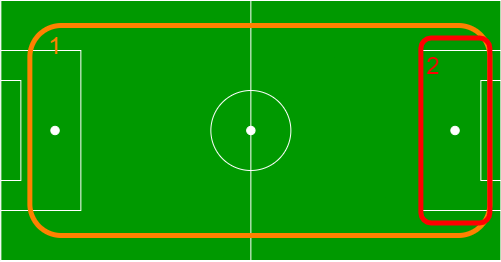
\includegraphics[width=12cm]{../img/schemaPonderationDef.png}
    \caption{Comparaison Arrêts et Tacles}
    \label{fig:comparaisonArretsTacles}
\end{figure}

Dans un match de foot, un tacle peut être effectué partout sur le terrain (voir zone 1 sur figure \ref{fig:comparaisonArretsTacles}) tandis qu'un arrêt est forcément effectué dans la zone dangereuse (zone 2) et il a, la plupart du temps, été effectué après avoir subi une attaque dangereuse. C'est pourquoi pour moi les tacles ont plus d'impacts défensif que des arrêts. Lors d'un match, le gardien peut ne faire aucun arrêt si son équipe a un niveau défensif élevé et qu'ils empêchent totalement l'équipe adverse d'effectuer des actions dangereuses. 

Ensuite, certaines statistiques défensives agissent comme des malus sur le score défensif (par exemple : les fautes) et d'autres comme des bonus. Contrairement au score offensif ou toutes les statistiques agissent positivement sur le score

Pour finir, j'ai fait une analyse sur la corrélation entre les tacles, les fautes et les cartons jaunes. Un carton jaune est donné à un joueur ayant effectué une faute qui a préalablement effectué un tacle.

\begin{figure}[H]
    \centering
    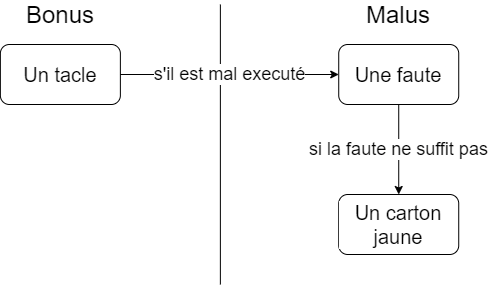
\includegraphics[width=15cm]{../img/schemaTacleFaute.png}
    \caption{Corrélation Tacles - Fautes - Cartons Jaunes}
    \label{fig:correlationTacleFaute}
\end{figure}

Comme on peut le comprendre sur la figure \ref{fig:correlationTacleFaute}, il faut qu'une faute annule complètement les points apportés par un tacle. Il va donc falloir utiliser la même pondération pour les deux statistiques et le carton intervient en malus supplémentaire si le tacle est mal executé.

J'ai choisi une pondération de 3 pour les tacles et donc pour les fautes et une pondération de 2 sur les cartons jaunes. La pondération des cartons ne doit pas être plus grande que celle des fautes, car les fautes annulent déjà complètement les points des tacles. 

À noter qu'il y aura théoriquement systématiquement plus de tacles que de fautes et plus de fautes que de cartons jaunes (ou égal mais jamais moins).

$n_{Tacles} >= n_{Fautes} >= n_{Cartons}  $

Quelques calculs pour mieux comprendre :
Une équipe a 117 tacles, 50 fautes et 17 cartons jaunes de moyenne par match\footnote{Ces chiffres ont été pris de manière aléatoire}. Il y a 3 de pondération pour les tacles et les fautes et 2 pour les cartons jaunes.

$Points = n_{Tacles} * Pond_{Tacles} - (n_{Fautes} * Pond_{Fautes} + n_{Cartons} * Pond_{Cartons})$ 


Pour rappel $Pond_{Tacles}=Pond_{Fautes}$, donc maintenant si on y met les chiffres cela donne : 

$167 = 117 * 3 - (50 * 3 + 17 * 2)$

Maintenant pour un cas ou l'équipe a quasiment autant de fautes que de tacles soit 200 tacles, 195 fautes et 23 cartons jaunes : 

$-31 = 200 * 3 - (195 * 3 + 23 * 2)$

On peut donc apercevoir que les points sont négatifs et qu'ils vont agir comme un malus sur le score défensif.

Pour finir, je vais montrer le classement que j'ai pu établir pour les statistiques défensives (du plus important au moins important) :
\begin{itemize}
    \item Bonus
    \begin{enumerate}
        \item Tacles (3)
        \item Arrêts (1)
    \end{enumerate}
    \item Malus
    \begin{enumerate}
        \item Nombre de buts encaissés (8, autant que pour le score offensif)
        \item Fautes (3)
        \item Cartons jaunes (2)
    \end{enumerate}
\end{itemize}

\noindent\textbf{Score sur la forme du moment}

En ce qui concerne la forme du moment des équipes, les 5 derniers matchs sont sélectionnés (si il y en a moins que 5 on prend le plus possible) et on fait une moyenne des points obtenus par match.\footnote{3 pts pour une victoire, 1 pt pour une égalité et 0 pts pour une défaite. Addition des points sur chaque match puis on fait une moyenne.} 
Au niveau du choix de la pondération sur la statistique des points obtenus par match, une victoire a plus d'impact sur le niveau de l'équipe qu'un nombre de buts conséquents. Une équipe peut gagner tous ces derniers matchs "1-0" en jouant efficacement sans chercher à marquer plein de buts tandis qu'une autre peut avoir 2 buts par match en moyenne mais elle ne gagne pas un seul match.

J'ai mis la pondération à 13 pour le nombre de points obtenus par match. La forme du moment est limité aux 5 derniers matchs donc un maximum de 15 points * 13.

\subsection{Réussite sur les prédictions}
\label{test_pourcent_reussite}

Pour pouvoir tester mes prédictions et voir le pourcentage de réussite de mon algorithme, il m'a été conseillé par M. Garcia de récupérer les données des matchs des années précédentes (informations du match et les statistiques) et de pouvoir faire une prédiction sur chacun de ces matchs. C'est très utile dans mon cas car je n'ai pas besoin d'attendre le résultat des matchs comme je sais déjà qui est le vainqueur.

J'ai tout d'abord cherché l'endpoint de l'API qui me permettrait de pouvoir récupérer les matchs et les statistiques de chacun d'eux. Et il s'avère que l'endpoint \texttt{Events} permet de faire cela. De plus, on a les statistiques directement pour chaque match (pas besoin de passer par l'endpoint \texttt{Statistics}). 

Initialement, la base de données ne ressemblait pas à ça (voir fig. \ref{fig:schemaDB}). J'envisageais uniquement de stocker les prédictions, rien de plus. Mais après la suggestion de M. Garcia, que j'ai au passage appliqué directement, j'ai ajouté les tables "match" et "statistic". Cependant, je n'ai pas utilisé les mêmes noms de colonnes que celle de l'API. En effet, selon moi, appeler ses colonnes "match\_id", ou encore "match\_hometeam\_name" n'est pas une bonne norme. Surtout que je vais devoir faire des requêtes SQL et je n'ai pas envie que mes requêtes ressemblent à \texttt{SELECT match.match\_id FROM match}.

Ensuite, j'ai du insérer les données en base avec un script en prenant les données de l'API. Cependant, il y a tout de même un soucis avec l'endpoint \texttt{Events} qui est que le nombre de données envoyées par l'API est trop conséquent donc il arrive parfois que l'insertion ne se passe pas correctement. Il faut alors faire une requête qui réduit la quantité de données envoyées par l'API (une ligue en particulier et les matchs d'une saison). 

Enfin pour tester, il m'a fallu faire un script qui récupère les matchs de la saison 2019-20 dans les 5 championnats majeurs et qui fait une prédiction sur chacun d'eux. Ce script m'a permis aussi de pouvoir choisir le bon delta pour la détermination d'une égalité sur un match (voir fig. \ref{fig:pourcentReussite}). 

\begin{figure}[htp]
    \centering
    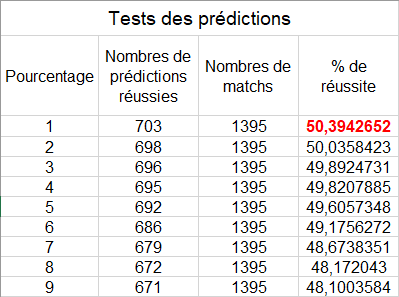
\includegraphics{../img/pourcentReussitePredictionV3.png}
    \caption{Pourcentage de réussite des prédictions}
    \label{fig:pourcentReussite}
\end{figure}

\subsection{Élaboration de prédictions sur une compétition}
\label{predictionCompetition}
Pour ce qui concerne les compétitions, je me suis dit qu'il fallait faire un constructeur qui récupère toutes les équipes du championnat sélectionné et qui forme un classement avec ces équipes. On y stockerait les victoires, les égalités, les défaites ainsi que les points. Pour l'historique de matchs, j'avais initialement prévu de stocker l'historique pour chaque équipe mais cela créerait des données en double. J'ai donc gardé le choix de faire un historique global des matchs et ensuite on cherche dedans les matchs d'une équipe X. 
Ensuite, une méthode qui fait une prédiction pour chacun des matchs de la compétition. Pour diminuer le temps de calcul, j'ai pensé faire du multiprocessing pour faire des prédictions en parallèles les une des autres. Il n'y a pas d'intérêt de faire du séquentielle puisque une prédiction n'est pas du tout dépendante d'une autre.

Donc dans cette classe, je prévois de stocker une variable qui contient le classement de la compétition et une autre qui contient l'historique de tout les matchs de la compétition.

\newpage

\section{Environnement de développement}

Pour ce qui concerne mon environnement de développement, j'ai décidé d'utiliser un Windows Subsystem for Linux\footnote{\url{https://fr.wikipedia.org/wiki/Windows_Subsystem_for_Linux}}. Une des plus-value d'un WSL est de pouvoir installer des paquets très facilement via les commandes shell. J'ai choisi comme distribution Debian pour sa stabilité, pour son système de gestion de paquets, et pour l'expérience que j'avais déjà avec cette distribution.  Pour ce qui concerne l'installation de nouveaux paquets, l'installation est très rapide et plus simple que sur Windows. De plus, Python est installé nativement avec la distribution.

Ensuite, j'ai utilisé un venv\footnote{Virtual environment ou environnement virtuel}. Cela va crée un environnement d'interprétation spécifique pour le projet en question. Ce venv est ensuite isolé des autres projets Python que l'on développe. 
Cela a plusieurs avantages. Si j'utilise une version d'une librairie en version 1.9 sur un projet et que j'ai un autre projet ou j'utilise cette même librairie en 1.10, cela va créer des soucis pour l'interprêteur Python car il ne sait pas différencier les versions se trouvant dans le répertoire "site-packages". Les deux versions de la librairie auront le même nom dans le même répertoire et cela créerait des soucis sur l'un de nos deux projets.
Ensuite, un des autres avantages vient avec le gestionnaire de paquets Python : pip. Effectivement, la commande \texttt{freeze} du gestionnaire, après avoir créé le venv, permet de sortir toutes les dépendances du projet que nous développons avec leurs versions\footnote{Taper la commande en dehors de l'environnement virtuel, affichera tous les paquets Python installé sur notre machine.}. C'est très utile pour faciliter l'installation du projet.
Dans mon cas, j'ai exporté toutes les dépendances avec leurs versions dans un fichier nommé \texttt{requirements.txt} et pour installer toutes les dépendances du projet, il suffit de taper la commande :
\noindent\texttt{pip3 install -r requirements.txt}

Pour faire l'installation complète du projet, suivez les instructions contenues dans le \texttt{README} situé à la racine du projet.

\newpage

\section{Développement Python}

\subsection{Appel à l'API}

Comme expliqué dans le point \ref{recupMatchStats}, il m'a été conseillé d'utiliser le design pattern \texttt{Façade}. Le principe de ce design pattern est de simplifier l'accès à un système complexe (l'API ici).

\lstinputPython{requests-getAction}

Cette fonction est généraliste pour permettre d'être appelé par tout les endpoints. Elle retourne une liste ou un dictionnaire selon l'endpoint appelé. À la ligne 8, il faut décoder la réponse en UTF-8 car en Python ce qui transite sur le réseau et du texte encodé en byte (\texttt{b''}). 
Elle vérifie aussi que le retour de l'API ne contient pas d'erreur. Pour expliciter la chose, quand l'API retourne une erreur 404 (exemple sur le listing \ref{erreurAPI}\footnote{À noter que l'erreur 404 n'est pas une "Authentification failed" mais une erreur "Not Found". C'est une erreur des développeurs de l'API. }), la librairie \texttt{requests} comprend que c'est un \texttt{status\_code} 200. C'est pour cela que je vérifie que le contenu contient la clé nommée "error" pour savoir si la requête est bonne ou non. Si elle n'est pas bonne, je lance une exception. Je fais la même vérification pour un code obtenu de la part de la librairie.
De plus, je fais des logs pour pouvoir avoir une traçabilité sur les requêtes faites à l'API et les potentielles erreurs qui peuvent apparaître.

\begin{lstlisting}[language=json, firstnumber=1, caption=Retour d'une erreur de l'API, captionpos=b, label=erreurAPI]
{
  "error": 404,
  "message": "Authentification failed!"
}
\end{lstlisting}

\lstinputPython{getH2H}

La méthode spécifie l'action pour l'API ( dans notre cas \texttt{get\_H2H} ) avec les paramètres spécifique à l'endpoint.
J'ai essayé de faire un code qui permet d'être facilement extensible pour ajouter de potentiels nouveaux endpoints. Pour conclure sur le code pour la communication avec l'API, je pense avoir fourni une classe respectant le design pattern \texttt{Façade} et suffisament extensible ce qui me permet de gagner du temps sur l'ajout de nouveaux endpoints.

\subsection{Gestion de la base de données}

La base de données est gérée par la classe \texttt{DbManager}. Dans cette classe, j'ai aussi opté pour une méthode généraliste pour la récupération de données stockées dans la base.

\lstinputPython{query}

Comme indiqué dans les commentaires de la méthode, les requêtes \texttt{INSERT}, \texttt{UPDATE} ou \texttt{DELETE} ne fonctionneront pas avec cette méthode car il manque la méthode \texttt{commit()} de sauver les changements faits sur la table en question. Le \texttt{fetchall()} permet de retourner toutes les lignes de la requête qui a été faite.

\lstinputPython{query-used}

Dans cette méthode, on voit bien que j'utilise la méthode du listing \ref{list-query} à la dernière ligne. Le fait de créer des méthodes généralistes comme celle du listing \ref{list-query} permet de simplifier la lecture du code. Ici, j'ai une méthode qui accepte des paramètres vides et je vérifie si ces derniers contiennent quelque chose, si oui, j'inclus les paramètres donnés dans la requête.

\lstinputPython{insert-prediction}

Le listing \ref{list-insert-prediction} contient le code pour insérer une prédiction en base. On peut voir directement que certains paramètres sont \texttt{NULL} par défaut. Cela s'explique par le fait que des prédictions hypothétiques vont être stockées en base. Ensuite, un autre point de comparaison que l'on peut faire par rapport à la méthode présente sur le listing \ref{list-query} est qu'ici, je fais un try catch pour récupérer une potentielle erreur lors de l'insertion. Ici, comme c'est un statement qui va changer la table \texttt{prediction}, on voit qu'à la fin du \texttt{try} de la méthode on fait un \texttt{self.\_\_db.commit()} (c'est le principe de transaction mais dans ce cas, on utilise pas tout les bénéfices de ce principe). Cette ligne permet de sauvegarder les changements qui ont été fait sur la base de données. On peut aussi remarquer que, contrairement aux \texttt{SELECT} statements, je fais des logs. J'ai choisi d'en faire uniquement sur les statements qui modifient la table.  
On peut se poser la question aussi sur le fait que l'API est techniquement aussi des \texttt{SELECT} statements donc pourquoi est-ce que j'ai aussi fait des logs pour ce service? Tout simplement, parce que l'API n'est pas mon service donc je préfère garder une trace sur les requêtes faites à cet outil externe.

\subsubsection{Transaction}

Une transaction\footnote{\url{https://openclassrooms.com/fr/courses/1959476-administrez-vos-bases-de-donnees-avec-mysql/1970063-transactions}} est très utile dans mon cas pour éviter les erreurs d'insertion de données qui sont liés entre elles dans ma base. Ici, pour insérer un match en base et pour insérer les statistiques qui lui sont liés. Il faut \textbf{absolument} en faire une pour éviter que des statistiques soient ajoutées alors que le match ne l'a pas été.


\lstinputPython{insert-match-with-stats}

Pour un match, on insère chaque statistique dans la table "statistic". Si aucune erreur est apparu, on sauvegarde les changements dans la base. La transaction est un bloc de dix requêtes. Elle contient l'insertion du match et 9 insertions de statistiques. Et contrairement au listing \ref{list-insert-prediction}, on fait un \texttt{rollback()}. Le rollback permet d'annuler les requêtes faites auparavant et on le fait lorsque l'on détecte une erreur sur un \texttt{INSERT} statement.

\subsection{Provider}

Le travail du \texttt{Provider} est d'être l'intermédiaire entre la classe \texttt{Prediction} ou la vue et l'API ou la base de données. Il met les données reçues de l'API dans le bon format pour la classe qui établira les pronostics. 

\lstinputPython{get-all-stats-from-teams-api}

Dans ce code, le but est de récupérer les résultats des derniers matchs entre deux équipes. Comme spécifié dans le point \ref{recupMatchStats}, certains matchs n'ont pas toutes les statistiques requises. c'est pourquoi pour chaque match, après avoir récupéré les statistiques pour chacun d'eux, j'appelle la méthode \texttt{\_\_check\_array\_is\_in\_other\_array()} qui me permet de vérifier que toutes les statistiques sont présentes pour chaque match, si elles n'y sont pas, on ne prend pas en compte ce match pour l'élaboration de la prédiction. Si toutes les statistiques sont là, on appelle la méthode qui insère les données du match dans le tableau lui correspondant. (soit \texttt{firstTeam\_VS\_secondTeam}, soit \texttt{firstTeam\_lastResults}, soit \texttt{secondTeam\_lastResults})

Avant tout ça, on vérifie tout de même que l'on ait des matchs récents. Du côté de l'API, si on donne l'un des noms des équipes de manière incorrecte, l'une des deux équipes n'aura pas de matchs ce qui est problématique pour établir un pronostic. 

\newpage

\lstinputPython{get-all-stats-from-teams-db}

Comme indiqué dans le point \ref{test_pourcent_reussite}, la structure de ma base de données est différente de celle de l'API ce qui fait que j'ai une méthode pour chaque source de données que j'utilise (soit ma base, soit l'API). Le listing \ref{list-get-all-stats-from-teams-api} et le listing \ref{list-get-all-stats-from-teams-db} retournent les données sous le même format. Les conditions ont le même but mais sont tout de même différentes du à la structure différente entre les sources de données. 

Autrement, les autres méthodes sont des appels à des endpoints de l'API ou des requêtes à la base de données en utilisant la façade ou la classe de gestion de la base de données.

Finalement, le \texttt{Provider} utilise le design pattern Singleton\footnote{\url{https://en.wikipedia.org/wiki/Singleton_pattern}}. En effet, comme je vais utiliser le Provider dans la classe Prediction mais aussi dans la vue pour pouvoir faire des requêtes à l'API ou à la base de données (voir fig. \ref{fig:architectureClasse})

\lstinputPython{singleton-provider}

Contrairement, à toutes mes autres classes, ici, je dois appliquer un singleton avec l'instruction \texttt{\_\_new\_\_()}. La différence entre \texttt{\_\_new\_\_()} et \texttt{\_\_init\_\_()} est que \texttt{\_\_new\_\_()} crée l'instance et la retourne, tandis que \texttt{\_\_init\_\_()} est appelé après le \texttt{\_\_new\_\_()}, ce qui veut dire que l'instance existe déjà et on ne retourne pas l'instance de l'objet. L'instruction \texttt{super()} appelle le constructeur de la classe parent (dans notre cas, on hérite d'\texttt{object})

\subsubsection{Cache des appels faits à l'API}
\label{cacheAppelsAPI}

La méthode du \texttt{Provider} qui intègre du cache lors d'appels à l'API est \texttt{get\_all\_stats\_from\_teams()}. Cette méthode a été implémenté pour éviter de surcharger l'API d'appels inutiles qui ont déjà été effectués dans la journée.

\lstinputPython{get-all-stats-from-teams}

Dans cette méthode, on regarde d'abord si un appel avec les deux équipes sélectionnées a été fait aujourd'hui, si c'est le cas, on va récupérer ces données dans la base (on verra dans la partie suivante qu'après chaque appel à l'API, on stocke les données de l'appel en base). À noter qu'on fait un \texttt{try except} car la méthode pour récupérer toutes les données en base peut retourner une Exception s'il manque des statistiques ou des matchs. Dernière chose, on fait un \texttt{await asyncio.sleep(0)} car on est obligé d'effectuer au minimum un await dans une méthode \texttt{async} (autrement, cela ne sert à rien de faire une méthode async). Dans le cas ou nous avons les données en base, aucun \texttt{await} n'a été fait.

Maintenant, passons au cas ou aucun appel a été fait aujourd'hui. On attend la réponse de la méthode asynchrone qui récupère les données depuis l'API. Une fois, cela fait, on va stocker en base le fait qu'on ait appelé l'API et on va stocker les matchs récupérées en base.

\subsection{Création d'une prédiction}

La création de la prédiction nécessite le nom des deux équipes et facultativement une date de début et une date de fin. Ce deux derniers paramètres permettent de spécifier à partir de quand doit on récupérer les données des derniers matchs. Ils sont utilisés pour tester la réussite des prédictions.

\lstinputPython{prediction-init}

Lors de l'instanciation de la classe \texttt{Prediction}, cette dernière récupère les données des matchs précédents et insère les données dans la classe \texttt{TeamResult} qui est créé dans le même fichier que la classe \texttt{Prediction}. \texttt{Prediction} contient deux objets \texttt{TeamResult}, une pour la première équipe et une pour la deuxième. Pour l'insertion de ces données, on fait aussi un try catch car les méthodes que l'on appelle peuvent lancer des exceptions du au nombre de matchs peu conséquent pour établir une prédiction.

\texttt{TeamResult} contient uniquement du stockage de données par rapport aux résultats des matchs précédents de chacune des équipes. Les uniques méthodes qui y sont contenu sont des méthodes pour retourner la moyenne de chacune des statistiques.

La méthode qui nous intéresse le plus pour cette classe est \texttt{define\_winner()} (voir list. \ref{list-prediction-define-winner}). C'est la méthode qui nous retournera le nom de l'équipe gagnante. Cette méthode est claire et limpide car elle fait uniquement une comparaison du score final des deux équipes après l'avoir calculé via les méthodes qui calculent les scores offensifs, défensif et le score de la forme du moment. 
Cependant, comme on peut le voir à la ligne 20, la comparaison n'est pas seulement une vérification si le score est plus grand que l'autre. En effet, il ne faut pas oublier que dans un match de football, il y a aussi le cas d'égalité. C'est pourquoi je vérifie si l'une des deux équipes a un score plus élevé que celui de son adversaire augmenté par un delta (qui est stocké dans le fichier \texttt{constants.py}). Le delta n'a pas été choisi de manière arbitraire (voir fig. \ref{fig:pourcentReussite}). Le cas d'égalité ne peut pas être vérifié uniquement avec un $score_{equipe1} == score_{equipe2}$. Cela s'explique par le fait que les chiffres que l'on manipule sont des doubles et que cela va être très rare d'avoir exactement le même nombre sur cette comparaison.

\lstinputPython{prediction-define-winner}

\subsubsection{Calcul des scores}

Pour le calcul du score offensif (voir list. \ref{list-prediction-compute-off-score}), comme indiqué au point \ref{choixPondStat}, on fait la moyenne de chaque statistique (\texttt{average\_goal\_score\_per\_game()} par exemple) et on multiplie la valeur obtenue par la pondération que l'on a choisi lors de l'analyse. Toutes ces pondérations sont stockées dans le fichier de constantes de l'application (voir l'aperçu des constantes list. \ref{list-constants})
\lstinputPython{prediction-compute-off-score}

\lstinputPython{constants}
A savoir qu'il n'y pas réellement de constantes en Python, ce sont des variables normales que l'on peut tout de même modifier.

\subsection{Réussite sur les prédictions}

\subsubsection{Insertion des données en base}

Pour tester la réussite des prédictions (comme expliqué au point \ref{test_pourcent_reussite}), il faut d'abord pouvoir insérer des données dans la base. J'ai d'abord construit la requête d'insertion des données dans la base (voir list. \ref{list-insert-match-with-stats}). Ensuite, j'ai fait le script qui insèrent les derniers matchs.

\lstinputPython{load-data-in-db}

Dans ce code, je récupère chaque donnée qui me sont importantes pour un match et j'appelle la méthode \texttt{save\_match\_with\_stats()} du Provider. Cette méthode fait le lien entre le Provider et la méthode du listing \ref{list-insert-match-with-stats}. Je vérifie quand même que le match ait un score et des statistiques avant l'ajout en base.

\subsubsection{Script de test}
Pour pouvoir utiliser ce script, il faut d'abord changer la manière de récupérer les données dans la classe \texttt{Prediction}. Au lieu de récupérer les statistiques depuis l'API, il faut les récupérer dans la base de données. Évidemment, il faut aussi avoir des données en base autrement, les prédictions ne fonctionneront tout simplement pas.

Le script suivant permet de tester le taux de réussite des prédictions en prenant entre, par exemple, le 9 août 2019 et le 28 juillet 2020. Il permet aussi de trouver le meilleur delta de détermination d'égalité. On récupère les matchs de entre ces deux dates. Pour chacun de ces matchs, on crée une prédiction qui récupérera les données des matchs d'il y a 6 mois et on compare le résultat de la prédiction avec le vrai résultat du match.
\lstinputPython{test-success-prediction}


\subsection{Classe de compétition}

\subsubsection{Constructeur}

Pour rappel, la classe \texttt{Competition} a pour but de faire une prédiction sur une compétition complète. Cela permet d'avoir un aperçu du résultat d'une compétition.

Pour cette classe, le constructeur contient la récupération des équipes d'une ligue et l'instanciation de la variable de classement. Dans cette liste, on y met un dictionnaire contenant les données spécifiques à chaque équipe (victoires, égalités, défaites, badges, noms, etc.) dans la compétition.

\lstinputPython{competition-ctor}

\subsubsection{Multiprocessing de tous les matchs}
\label{multiprocessing}

Dans la méthode \texttt{compute\_competition()}, comme expliqué dans le point \ref{predictionCompetition}, je trouvais important de faire du multiprocessing pour calculer parallèlement le vainqueur de tous les matchs d'un championnat. J'ai choisi d'utiliser la librairie \texttt{multiprocessing} et d'utiliser la classe \texttt{Process}.
Pour commencer, je crée toutes les possibilités de matchs\footnote{Il y en a 190 car mon application ne prend pas en compte le fait que le match soit joué à domicile donc il n'y a pas besoin de faire les matchs aller-retour}. Ensuite, je crée un \texttt{Process} par match. Chaque process appelle la méthode \texttt{make\_prediction()} qui crée la prédiction et insère le résultat dans la liste de sortie\footnote{Cette liste doit être crée avec la classe \texttt{Manager} de la librairie multiprocessing car la liste de cette classe est partagée par tous les process. Autrement, le stockage des données ne se fera pas correctement.}. Je cherchais une manière rapide de créer toutes ces prédictions et le multiprocessing est la chose qui me fallait. Le multithreading aurait faciliter le partage des données entre les process mais lorsque je l'ai testé, il prenait le même temps que la manière séquentielle.\footnote{\url{https://datanoon.com/blog/multiprocessing_in_python/}}
Je fais tout de même un \texttt{time.sleep()} de 100 millisecondes entre chaque lancement de process en guise de sécurité surtout pour éviter de trop saturer la base de données ou l'API.
Enfin, je vérifie que tous les process soient bien finis pour retourner l'historique des matchs.

À noter que le code ci-dessous contient du code en commentaires qui permettait de voir la performance du parallèlisme.

\lstinputPython{compute-competition}

\subsubsection{Retour du classement du championnat}

Le retour du classement se fait après avoir appelé la méthode \newline \texttt{compute\_competition()}.

Pour le retour du classement de la compétition, je dois parcourir le classement des équipes et chercher dans l'historique des matchs pour compter les victoires, égalités, défaites et ainsi compter les points pour les équipes dans le classement. Pour finir, le classement est trié par nombre de points de chaque équipe de manière décroissante. Pour ce qui concerne la méthode \texttt{sorted()}, la clé est là pour spécifier avec quoi on doit trier.

\lstinputPython{get-standings}

\subsubsection{Problème de donnée de l'API}
Il y a eu un soucis rencontré lors du développement de cette fonctionnalité\footnote{Ce problème est présent sur toutes les fonctionnalités mais il a été découvert lors du développement des compétitions}. L'API n'est pas cohérente sur les données qu'elle transmet. Je m'explique :
Dans le code du constructeur, je récupère toutes les équipes de la compétition sélectionnée. Ces équipes seront ensuite utilisées pour créer les compétitions\footnote{Pour rappel, je récupère les derniers résultats de chaque équipe via l'endpoint H2H de l'API et ce dernier fonctionne \textbf{uniquement} avec le nom des équipes}. Cependant, le soucis que j'ai pu rencontré est le fait que l'API me donne comme donnée "Manchester United" à la récupération des équipes d'une compétition. Et pour l'endpoint H2H, en passant en paramètre "Manchester United", on reçoit des matchs de 2018, ce qui est inutile pour faire nos prédictions. Cependant, on reçoit des résultats, quand on met le nom "Manchester Utd", datant de 2021.


\begin{lstlisting}[language=json, firstnumber=1, caption=Aperçu du JSON avec "Manchester United", captionpos=b, label=apercuJSONUnited1]
// 20210525104030
// https://apiv2.apifootball.com/?action=get_H2H&
firstTeam=Manchester%20United&secondTeam=Newcastle&
APIkey=[...]

{
  "firstTeam_VS_secondTeam": [
    {
      "match_id": "134613",
      "country_id": "41",
      "country_name": "ENGLAND",
      "league_id": "148",
      "league_name": "Premier League",
      "match_date": "2018-10-06",
      "match_status": "Finished",
      "match_time": "18:30",
      "match_hometeam_id": "2627",
      "match_hometeam_name": "Manchester United",
      "match_hometeam_score": "3",
      "match_awayteam_id": "2630",
      "match_awayteam_name": "Newcastle",
      "match_awayteam_score": "2",
      "match_hometeam_halftime_score": "0",
      "match_awayteam_halftime_score": "2",
      "match_live": "0",
      "team_home_badge": "https://apiv2.apifootball.com/badges/
      2627_manchester-united.png",
      "team_away_badge": "https://apiv2.apifootball.com/badges/
      2630_newcastle.png",
      "league_logo": "https://apiv2.apifootball.com/badges/
      logo_leagues/148_premier-league.png",
      "country_logo": "https://apiv2.apifootball.com/badges/
      logo_country/41_england.png"
    },
    [...]
\end{lstlisting}

\begin{lstlisting}[language=json, firstnumber=1, caption=Aperçu du JSON avec "Manchester United", captionpos=b, label=apercuJSONUnited2]
// 20210525104515
// https://apiv2.apifootball.com/?action=get_H2H&
firstTeam=Manchester%20Utd&secondTeam=Newcastle&
APIkey=[...]

{
    "firstTeam_VS_secondTeam": [
    {
        "match_id": "411423",
        "country_id": "41",
        "country_name": "England",
        "league_id": "148",
        "league_name": "Premier League",
        "match_date": "2021-02-21",
        "match_status": "Finished",
        "match_time": "20:00",
        "match_hometeam_id": "2627",
        "match_hometeam_name": "Manchester Utd",
        "match_hometeam_score": "3",
        "match_awayteam_id": "2630",
        "match_awayteam_name": "Newcastle",
        "match_awayteam_score": "1",
        "match_hometeam_halftime_score": "1",
        "match_awayteam_halftime_score": "1",
        "match_live": "0",
        "team_home_badge": "https://apiv2.apifootball.com/badges/
        2627_manchester-united.png",
        "team_away_badge": "https://apiv2.apifootball.com/badges/
        2630_newcastle.png",
        "league_logo": "https://apiv2.apifootball.com/badges/
        logo_leagues/148_premier-league.png",
        "country_logo": "https://apiv2.apifootball.com/badges/
        logo_country/41_england.png"
    },
    [...]
\end{lstlisting}

On peut voir que l'id de l'équipe est le même mais que le nom est différent et surtout que les résultats sont totalement différents.

Pour régler ce soucis, je n'ai pas trouvé d'autre solution que d'avertir tout d'abord les développeurs de l'API de ce soucis de données et de gérer ce cas de bord spécifique dans le code avec une condition.

À noter que la version 3 de l'API est sortie et le soucis a été réglé. Cependant, les statistiques que j'utilise ont "disparu"\footnote{Elles n'ont pas réellement disparu mais elles sont liée à un joueur en particulier. Donc pour les avoir je vais devoir parcourir les statistiques de chacun des joueurs d'un match.} ce qui fait que je dois changer la manière de récupérer les statistiques dans le code. La version 3 de l'API est sortie le 20 mai 2021. De plus, la sortie de la V3 a été faite vers la fin de mon travail de diplôme et les délais sont trop courts pour pouvoir changer de version et modifier tout ce qui a déjà été développé. 

\subsection{De Multiprocessing à Asynchrone}
\label{multiprocessingToAsync}

Dans le point \ref{multiprocessing}, j'explique que j'avais besoin de paralléliser les prédictions pour augmenter les performances\footnote{Pour rappel, une prédiction met plus ou moins environ 8 secondes à se faire (appels à l'API inclus) }. J'ai donc pensé que la solution était de faire du multiprocessing (ayant fait des appels à l'API de manière synchrone, je ne voulais pas modifier tout le travail que j'avais déjà fait). J'ai donc développé le multiprocessing dans mon projet mais j'ai remarqué que lorsque c'était la première fois que je faisais une prédiction sur une compétition entière, les subprocess se bloquaient vers la fin du calcul de la prédiction. J'ai essayé de comprendre la raison mais débugger du multiprocessing est assez complexe. J'ai donc posé la question sur un groupe communautaire, s'il y avait une possibilité quelconque de débugger du multiprocessing, en expliquant le projet et ce que je cherche à faire avec le multiprocessing. Et des personnes de la communauté m'ont répondu que dans mon cas, la meilleure chose était de passer à de l'asynchrone. L'approche asynchrone était bien plus adapté à ce dont j'avais besoin. En effet, en réalité ce que je cherchais à faire avec le multiprocessing était d'éviter qu'on attende que les prédictions se fassent les unes après les autres (que le code se \textbf{bloque} sachant que le code prenait beaucoup de temps sur les appels de l'API) et donc de les faire toutes en parallèles. C'est clairement le but de l'asynchrone. De plus, le multiprocessing a un coût en ressources car il crée plusieurs interpréteurs indépendants.

Pour régler le soucis qui faisait bloquer les subprocess du multiprocessing, j'ai commencé par essayer de rendre asynchrone mes méthodes de haut niveau (les méthodes du Provider). J'ai commencé à le faire et je me suis vite rendu compte que l'asynchrone est nécessaire partout, car les appels à l'API étaient bloquant. J'ai donc du rendre tout mon code asynchrone. 

\textbf{Notez que tout le code aperçu plus haut qui contiennent des appels à l'API sont passés en asynchrone.}

\textbf{De plus, certaines méthodes ont été ajoutés suite à l'implémentation de l'asynchrone dans le projet.}

\subsubsection{Comment fonctionne l'asynchrone ?}

On a pu le voir brièvement dans le point \ref{cacheAppelsAPI} mais je vais l'expliquer plus clairement

\lstinputPython{async-get-match-infos}

Voici un exemple très court de l'utilisation de l'asynchrone en Python. Tout d'abord, la méthode doit avoir le mot-clé \texttt{async} et une méthode doit forcément passer par une instruction \texttt{await}. Si une méthode asynchrone ne passe pas par une instruction \texttt{await}, une Exception est déclenchée. L'instruction \texttt{await} attend la réponse de la méthode avant de passer à la suite. Lorsque l'on utilise l'instruction \texttt{await}, l'objet est un \texttt{awaitable}.
La plus grosse utilité est de le combiner avec la librairie \texttt{asyncio} et sa méthode \texttt{wait()}.

\lstinputPython{asyncio-wait}

Cette méthode permet de lancer plusieurs objects \texttt{awaitable}, qu'on appelle \texttt{Tasks}, simultanément. La méthode est finie lorsque toutes les \texttt{Tasks} sont finies\footnote{Un paramètre \texttt{return\_when} est présent et la valeur par défaut est \texttt{ALL\_COMPLETED}}. Le retour de cette méthode est deux sets de \texttt{Tasks}, un set avec les \texttt{Tasks} finies et l'autre avec les \texttt{Tasks} qui sont en attente ou en cours. Le paramètre est une liste utilisé grâce aux générateurs\footnote{\url{https://wiki.python.org/moin/Generators}}. 

\subsubsection{\texttt{Requests} à \texttt{Aiohttp}}

Après avoir compris que je devais changer tout le système d'appel à l'API en asynchrone, j'ai remarqué que la librairie que j'utilisais initialement ne permet pas de faire des appels HTTP asynchrones. J'ai donc trouvé \texttt{aiohttp} qui permet de faire ces appels en asynchrone.

\lstinputPython{aiohttp-getAction}

En comparaison avec le listing \ref{list-requests-getAction}, le listing \ref{list-aiohttp-getAction} appelle l'API de manière asynchrone grâce à la librairie \texttt{aiohttp}\footnote{\url{https://docs.aiohttp.org/en/stable/\#getting-started}}. Le statement \texttt{with} permet de gérer plus efficacement les Exceptions.

\subsubsection{Transfert des méthodes await dans une nouvelle méthode}

Auparavant, lorsque je devais créer une prédiction, j'appelais uniquement le constructeur de \texttt{Prediction} qui faisait l'appel au Provider. Cependant, maintenant que je suis passé sur de l'asynchrone, il faut utiliser l'instruction \texttt{await} qui fonctionne uniquement sur des méthodes \texttt{async}. Selon moi, ce n'est pas une bonne pratique de faire un constructeur qui est asynchrone. C'est pourquoi j'ai créé une fonction qui est asynchrone et qui appelle le Provider après avoir instancié l'objet de la classe.

\lstinputPython{async-make-prediction}

On peut voir qu'après avoir créé l'objet \texttt{Prediction}, j'appelle la méthode asynchrone \texttt{create\_prediction()} qui fait donc l'appel au Provider de manière asynchrone.

\newpage

\section{Développement Python Flask}

Python Flask est un framework web Python très rapide à prendre en main et très puissant. Il utilise Jinja2 pour le templating et Werkzeug pour faire la communication avec entre un serveur web et une application web. 

\subsection{Templating}

Le templating permet de créer des pages dynamiques selon les données que l'on donne à la page. Dans le cas de l'application, cela permet d'afficher ou non, certaines parties du site web selon les actions d'un utilisateur.

\subsection{Template parent du site web}

L'outil se prend en main rapidement et un des concepts qui facilite la vie est la possibilité de faire un template parent. Pour être plus clair, je vais avoir un fichier \texttt{competitions.html} qui va utiliser tout le contenu du fichier \texttt{base.html} mais qui va changer uniquement certaines parties, selon des instructions.

Ici, on a un aperçu du fichier \texttt{base.html} et on peut y voir des \texttt{ \{\% block header \%\}\{\% endblock \%\} }. Ces instructions permettent d'insérer du contenu depuis un fichier enfant. (voir list.  \ref{list-competitions}).

\lstinputHTML{base}

\lstinputHTML{competitions}

\begin{figure}[htp]
    \centering
    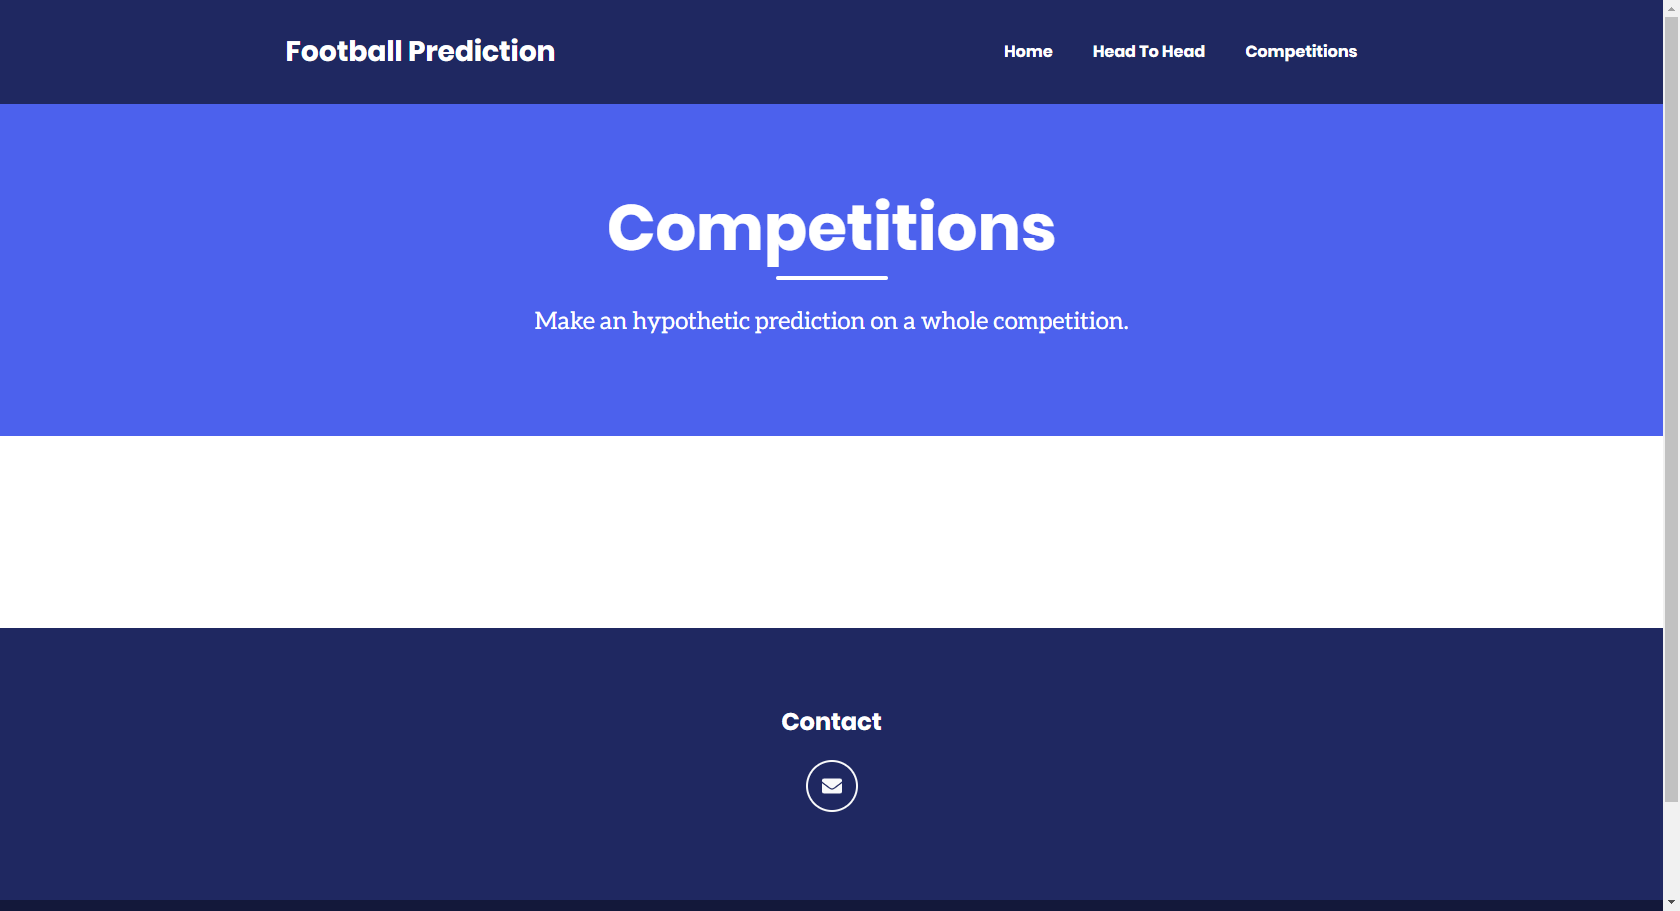
\includegraphics[width=15cm]{../img/apercuVueCompetitions.png}
    \caption{Vue Compétitions}
    \label{fig:vueCompetitions}
\end{figure}

\subsection{Routes}

Les routes avec Python Flask sont liées à des méthodes. Ces méthodes doivent forcément retourner quelque chose. L'instruction \texttt{@app.route("/index")} permet de dire la méthode qui suit sera liée à la route "/index". On peut aussi lié plusieurs routes à la même méthode. (voir list. \ref{list-app-index} ligne 1)

\lstinputPython{app-index}

Comme j'ai pu le dire précédemment, il faut obligatoirement retourner quelques choses. Cependant, j'ai aussi dit que j'utilisais le templating offert par Jinja2. Pour pouvoir profiter de ce templating, Flask a une méthode nommée \texttt{render\_template()}. Le premier paramètre est le fichier de template que l'on veut utiliser ensuite les autres paramètres sont des données que l'on veut transmettre à notre vue. Dans mon cas, je donne la liste des matchs précédents et la liste des matchs qui vont se jouer prochainement. J'expliquerais cette méthode de manière plus claire dans le point \ref{flaskAccueil}.

\subsection{Accueil}
\label{flaskAccueil}

La page d'accueil du site a pour but d'afficher les matchs précédent avec leur prédictions et le résultat du match. Cela permet à l'utilisateur de voir si l'application a correctement prédit le résultat du match. Ensuite, elle affiche aussi la prédiction sur les matchs qui arrivent dans les prochains jours. J'ai choisi de prendre les matchs qui vont se jouer dans les 3 prochains jours pour éviter d'avoir plusieurs matchs de la même équipe, car le résultat d'un match peut influencer le résultat d'un autre donc la prédiction peut changer après avoir disputer le premier match. De même pour les matchs précédents, j'ai choisi d'afficher les matchs datant d'il y a trois jours.

Pour des raisons de pertinences et pour éviter de potentielles erreurs, j'ai décidé d'afficher uniquement les matchs des championnats européens majeurs.

\subsubsection{Affichage des matchs précédents}

Sur le listing \ref{list-app-index}, on peut voir le procédé pour récupérer les matchs précédents. Tout d'abord, je déclare les variables pour les dates et ensuite, je vérifie que les matchs ne soient pas stockés dans mon cache. En effet, si je ne fais pas de cache, à chaque fois que je reviens sur la page d'accueil, l'application rechargera tout, ce qui n'est pas une bonne idée. Si rien est stocké en cache, je fais l'appel à la méthode qui me permet de récupérer tout les matchs précédent pour chacune des ligues que j'ai choisi. Celle-ci retourne un dictionnaire avec comme clé : le nom du championnat, et comme valeur : un tableau avec les matchs du championnat. 

Après cela, je vérifie qu'il y ait des matchs dans la réponse de la méthode (list. \ref{list-app-index} ligne 15). En effet, le contenu du retour contient forcément des clés mais il faut vérifie qu'au moins un des tableau contient un match. Cela permet d'afficher qu'il n'y a pas de prédictions pour les matchs précédents. Si on ne fait pas ça, l'accueil nous affichera chaque ligue sans match.

\lstinputPython{get-previous-matches-multiple-leagues}

J'ai décidé de mettre la méthode pour récupérer les prédictions des matchs précédents dans le \texttt{Provider}, car il n'y a que de la communication avec de la base de données.

Pour ce qui concerne le code de la vue, je vous invite à regarder le listing \ref{list-index-previous-matches}

\lstinputHTML{index-previous-matches}

\subsubsection{Affichage et création des prédictions pour les prochains matchs}

Encore sur le listing \ref{list-app-index}, on peut apercevoir la processus de récupération des prédictions sur les prochains matchs qui vont se jouer. Cependant, dans ce cas, contrairement à celui précédent, il faut récupérer les prochains matchs qui vont se jouer et établir une prédiction. Si une prédiction a déjà été créé, on ne fait que la récupérer.

\lstinputPython{get-upcoming-matches-predictions}

Cette méthode fait deux choses :
\begin{itemize}
    \item Elle récupère les prédictions d'une ligue sur les prochains matchs
    \item Elle crée les prédictions pour les prochains matchs
\end{itemize}

D'abord, on récupère les matchs qui ont déjà été prédit pour cet interval de temps et on crée un tableau avec les identifiants des matchs qui sont déjà stockés en base\footnote{Cela va permettre d'éviter de stocker à nouveau une prédiction en base.}. Ensuite, pour chaque prochain match\footnote{Les prochains matchs ont été récupérés grâce à l'endpoint \texttt{Events}}, je vérifie s'il y a du contenu dans la requête faite à la base de données (celle pour récupérer les prédictions déjà faites), et s'il n'y a rien dedans\footnote{Ce qui veut dire qu'aucun des matchs n'a de prédictions.}, on crée une prédiction pour ce dernier\footnote{\texttt{make\_prediction()} crée une prédiction et la sauvegarde en base.}. Autrement, on vérifie si le match en question a déjà une prédiction en base et si c'est le cas, on l'insère dans le tableau de retour.

À la ligne 33, on vérifie si l'identifiant est déjà présent dans \texttt{array\_match\_ids}. En effet, si mon match n'a pas de prédiction, il va m'en créer une. Cependant, le fait que je vérifie si le match a le même identifiant que celui de la prédiction dans une boucle qui est elle-même dans une boucle, cela implique qu'il faut s'assurer de ne pas recréer une prédiction qui a déjà été faite auparavant. Une fois que j'ai crée la prédiction, j'ajoute l'identifiant du match dans le tableau qui contient tous les ids des matchs qui ont une prédiction.

La méthode qui est appelé dans le listing \ref{list-app-index} est la suivante :

\lstinputPython{get-upcoming-matches-multiple-leagues}

Contrairement au listing \ref{list-get-previous-matches-multiple-leagues}, la méthode \texttt{get\_upcoming\_matches\_predictions()} se trouve pas dans le provider. Effectivement, j'ai trouvé plus judicieux de la mettre dans le fichier de routing plutôt que dans le provider, car dans le listing \ref{list-get-upcoming-matches-predictions}, on fait de la création de prédiction. Ce qui veut dire que dans le provider, un objet \texttt{Prediction} aurait été créé et ce dernier crée un objet \texttt{Provider}. 
 
Pour ce qui concerne le code de la vue, je vous invite à voir le listing \ref{list-index-upcoming-matches}.

\lstinputHTML{index-upcoming-matches}

\subsubsection{Aperçus}

\begin{figure}[htp]
    \centering
    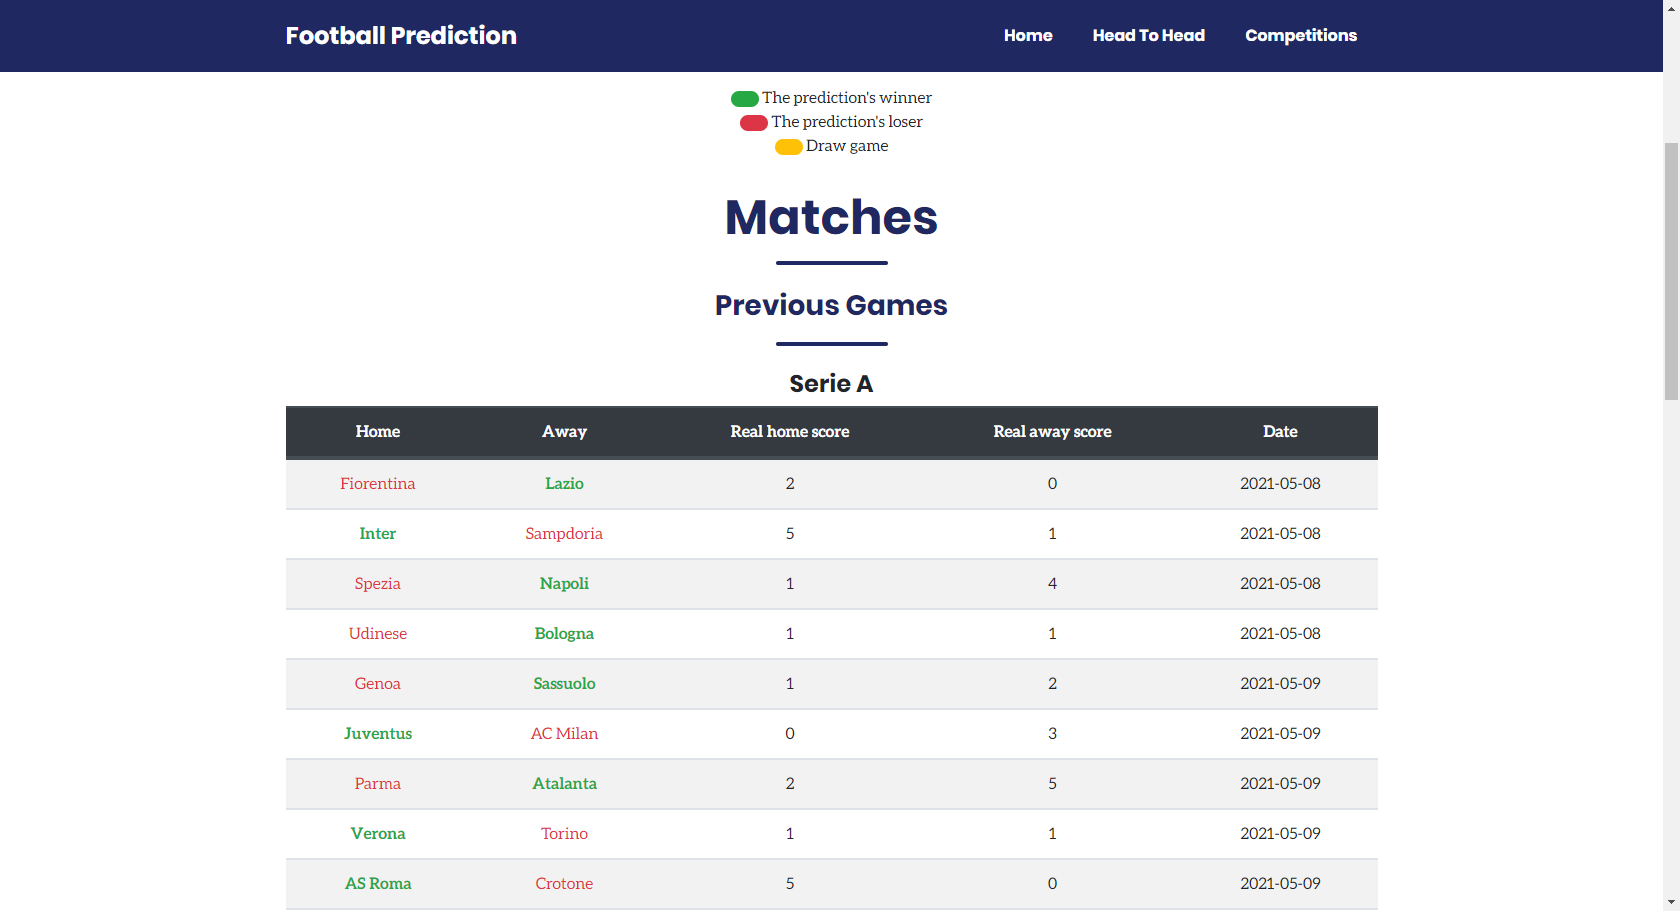
\includegraphics[width=28em]{../img/previousGamesAccueil.png}
    \caption{Aperçu de la page d'accueil - Matchs précédents}
    \label{fig:previousGamesAccueil}
\end{figure}

\begin{figure}[htp]
    \centering
    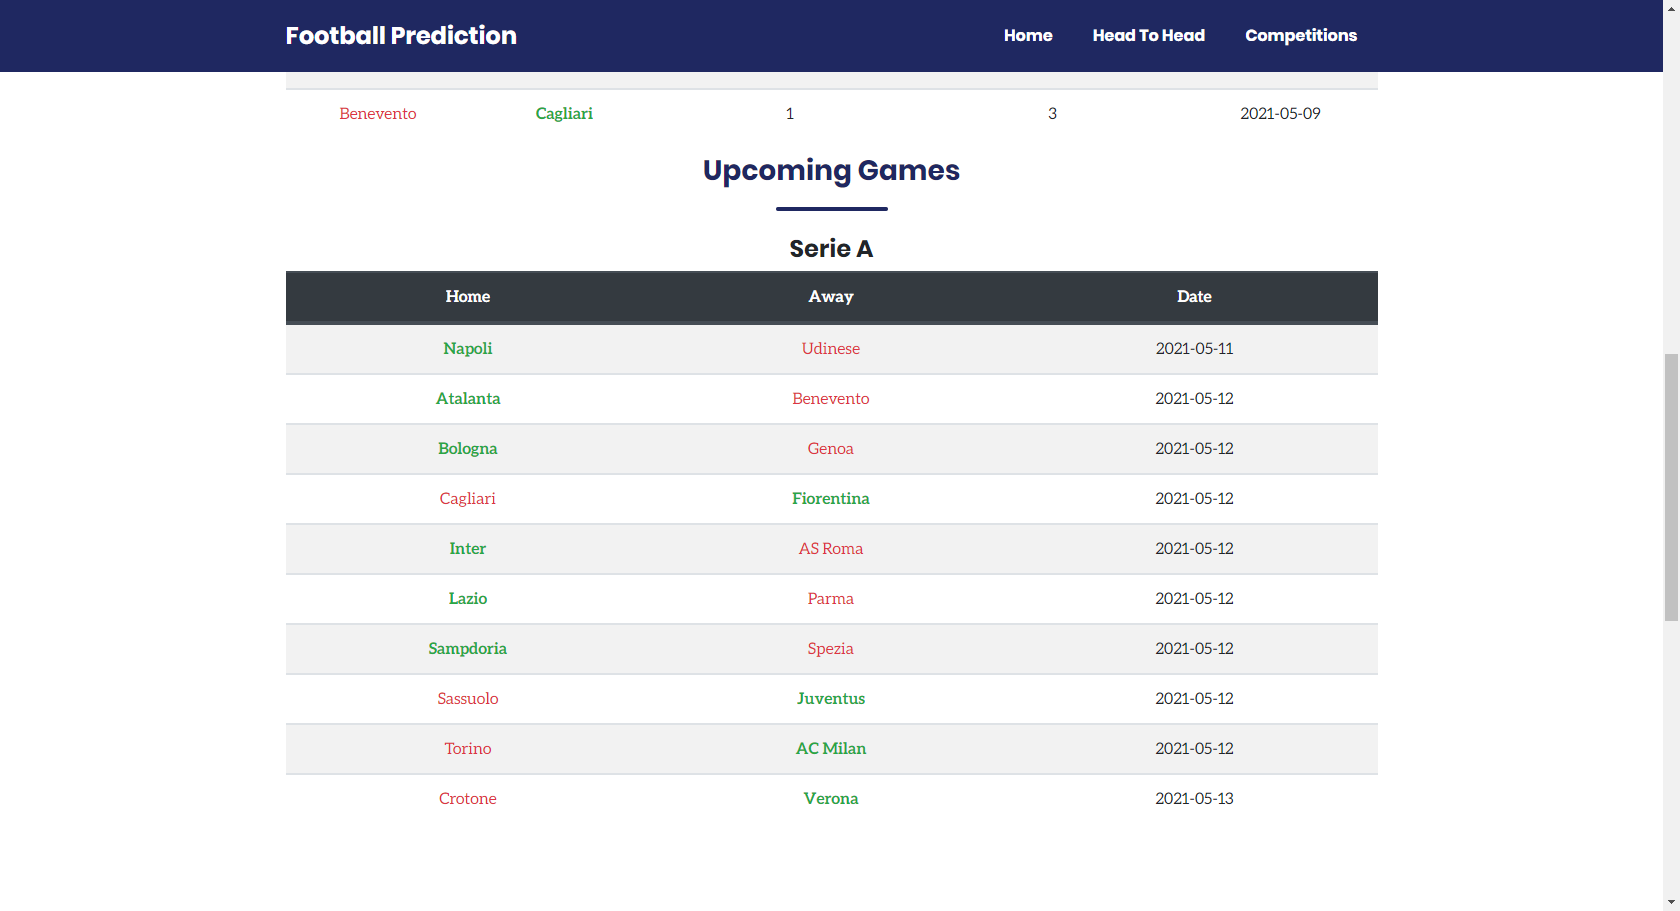
\includegraphics[width=28em]{../img/upcomingGamesAccueil.png}
    \caption{Aperçu de la page d'accueil - Prochains matchs}
    \label{fig:upcomingGamesAccueil}
\end{figure}

\subsection{Head To Head}

La fonctionnalité Head To Head permet de créer une prédiction hypothétique. L'utilisateur peut créer sa propre prédiction.

\subsubsection{Sélection de la ligue}
\label{selectionLigueH2H}

Pour commencer, je tiens à rappeler une des spécifications que l'on a au tout départ qui est "on ne peut pas faire de prédiction entre deux équipes de championnat différent"\footnote{Revoir la partie \ref{niveauDifferentChampionnats}.}. Ceci est très important pour la sélection de la ligue. En effet, il nous faut absolument l'identifiant de la ligue pour pouvoir savoir si la prédiction est valable ou non.

\lstinputHTML{league-modal}

Dans cette modal, on peut voir que le formulaire pointe sur la méthode \texttt{h2h\_league\_select} grâce à \texttt{url\_for()}. 

La méthode du listing \ref{list-h2h-league-select} récupère les données du formulaire et les transmet à la route qui est appelé lorsque l'on sélectionne une ligue. Cette route contient l'id de la ligue directement dans l'url. 

\lstinputPython{h2h-league-select}

La méthode du listing \ref{list-h2h-league-selected} vérifie que l'identifiant de la ligue est bien dans la liste des ligues majeurs européens, sinon, elle redirige l'utilisateur vers la page Head To Head. Ensuite, elle récupère les équipes qui font parties de ce championnat. Puis, elle formate les données de chaque équipe et trie le tableau des équipes dans l'ordre alphabétique par nom. Pour finir, elle insère la liste des équipes dans le cache et redirige vers la page \texttt{h2h.html} avec l'identifiant de la ligue et les équipes en paramètre.

\lstinputPython{h2h-league-selected}

\subsubsection{Sélection des équipes}

Pour la sélection des équipes, il y a deux formulaires (un pour la sélection de chaque équipe). Cependant, les deux formulaires ont la même action, soit \texttt{url\_for("h2h\_teams\_select")}. (voir list. \ref{list-h2h-first-team} pour un aperçu du formulaire)

\lstinputHTML{h2h-first-team}

Dans ce formulaire, il est important d'ajouter un input caché qui stockera l'identifiant de la ligue pour le garder tout au long de la création de la prédiction.

\lstinputPython{h2h-teams-select}

Tout d'abord, je récupère systématiquement l'identifiant de la ligue. Il me faut absolument cette information pour créer ma prédiction. Ensuite, comme je sélectionne toujours en premier l'équipe qui est à domicile, je n'ai pas besoin de vérifier s'il existe. Enfin, si j'ai uniquement l'identifiant d'une équipe, je renvoie vers la route \texttt{h2h\_one\_team\_selected} en donnant l'identifiant de l'équipe et l'identifiant de la ligue en paramètre. Autrement, je renvoie l'utilisateur vers la route \texttt{h2h\_two\_teams\_selected} en passant en paramètres les identifiants des deux équipes ainsi que l'identifiant de la ligue.

\lstinputPython{h2h-one-team-selected}

Lorsque l'on arrive sur la route où l'utilisateur a déjà sélectionné l'équipe qu'il voulait, on récupère le nom et le badge de l'équipe qu'il a sélectionné grâce à l'API et on affiche la page \texttt{h2h.html} en donnant en paramètres, l'identifiant de la ligue, les informations de l'équipes qu'il a sélectionné (sous forme de tableau) et on donne la liste des équipes de la ligue sélectionnée précedemment.

\lstinputHTML{h2h-second-team}

Comme on peut le voir sur le listing \ref{list-h2h-second-team}, on fait pareil qu'expliqué précédemment pour garder l'information sur la première équipe, c'est-à-dire qu'on cache l'identifiant de la première équipe dans un input caché\footnote{À savoir que cela ne sécurise pas du tout l'application, il faut tout de même vérifier lors de la création de la prédiction que tous les identifiants soient bons et cohérents.}.

L'action sur le deuxième formulaire est la même que le premier (list. \ref{list-h2h-teams-select}). Mais ensuite, on donne le travail à la route \texttt{h2h\_two\_teams\_selected()}. Cette route fait pareil que la route du listing \ref{list-h2h-one-team-selected} mais elle prend les informations pour les deux équipes.

\lstinputPython{h2h-two-teams-selected}

Finalement, une fois avoir sélectionné les deux équipes, on doit afficher le bouton pour créer la prédiction. (voir list. \ref{list-h2h-show-button-make-prediction})

\lstinputHTML{h2h-show-button-make-prediction}

\subsubsection{Création de la prédiction}

Tout d'abord pour afficher un chargement de la page pour l'utilisateur (et pour éviter qu'il pense que la page ne fonctionne plus), j'ai fait un peu de JS pour afficher un gif de loading, lorsque l'on clique sur le bouton "Make the prediction". 

\begin{lstlisting}[language=JavaScript, firstnumber=1, caption=Affichage du loading lors de la création de la prédiction, captionpos=b, label=jsLoading]
function loading() {
  $("#loading_div").show()
  $("#content").hide()
}
\end{lstlisting}

Ce code n'est écrit que quand le bouton "Make the prediction" est présent.

Maintenant, on passe à la partie de création de la prédiction après avoir sélectionné les deux équipes. Les données qui nous sont tramsmises sont des identifiants (voir list. \ref{list-h2h-show-button-make-prediction}).

La première chose qui est faite est de récupérer les données du formulaire (\texttt{leagueId}, \texttt{teamIdHome} et \texttt{teamIdAway}). Ensuite, on vérifie que les deux équipes ne soient pas les mêmes\footnote{Inutile de faire une prédiction entre Arsenal et Arsenal par exemple}. Ensuite, on vérifie que les équipes sélectionnées par l'utilisateur soit dans la ligue qu'il a sélectionné auparavant\footnote{En effet, comme les ids sont dans l'url de la page, l'utilisateur peut s'amuser à modifier ces identifiants et donc faire une prédiction infaisable.}. Une fois cette vérification faite, on nettoie les erreurs qui peuvent être stockées en cache et on récupère les informations des équipes (badge, nom, etc.). Après cela, on va récupérer les dernières prédictions entre les deux équipes et les formatter correctement. Après avoir fait cela, on va vérifier si dans les 3 derniers jours la prédiction a été faite, s'il y a une prédiction, c'est celle là qu'on affiche. En effet, cela permet d'éviter de regénérer une nouvelle prédiction chaque jour alors qu'une prédiction a déjà été faite dans les jours précédents. Finalement, s'il n'y aucune erreur, on retourne la page \texttt{h2h.html} avec les informations des deux équipes, le resultat de la prédictions et les derniers prédictions qui ont été faites entre les deux équipes.

\lstinputPython{h2h-make-prediction}

En ce qui concerne les éventuelles erreurs, lorsque je veux en afficher une, je la stocke dans le cache pour au final, rediriger l'utilisateur sur la page de départ de cette section. La page de départ gère ces potentielles erreurs. (voir list. \ref{list-h2h})

\lstinputPython{h2h}

\subsubsection{Informations complémentaires}
On pourrait réduire le nombre d'appels faits à l'API. Par exemple dans le listing \ref{list-h2h-two-teams-selected}, je refais un appel qui est déjà présent dans le listing \ref{list-h2h-one-team-selected}. J'aurais pu transmettre le dictionnaire après avoir fait le premier appel. Cependant, comme les données passent par l'url de la route, le dictionnaire serait présent dans l'url. De plus, l'utilisateur aurait accès à l'url des images, aux noms des équipes et il pourrait modifier ces données.

\subsubsection{Aperçus}

\begin{figure}[htp]
    \centering
    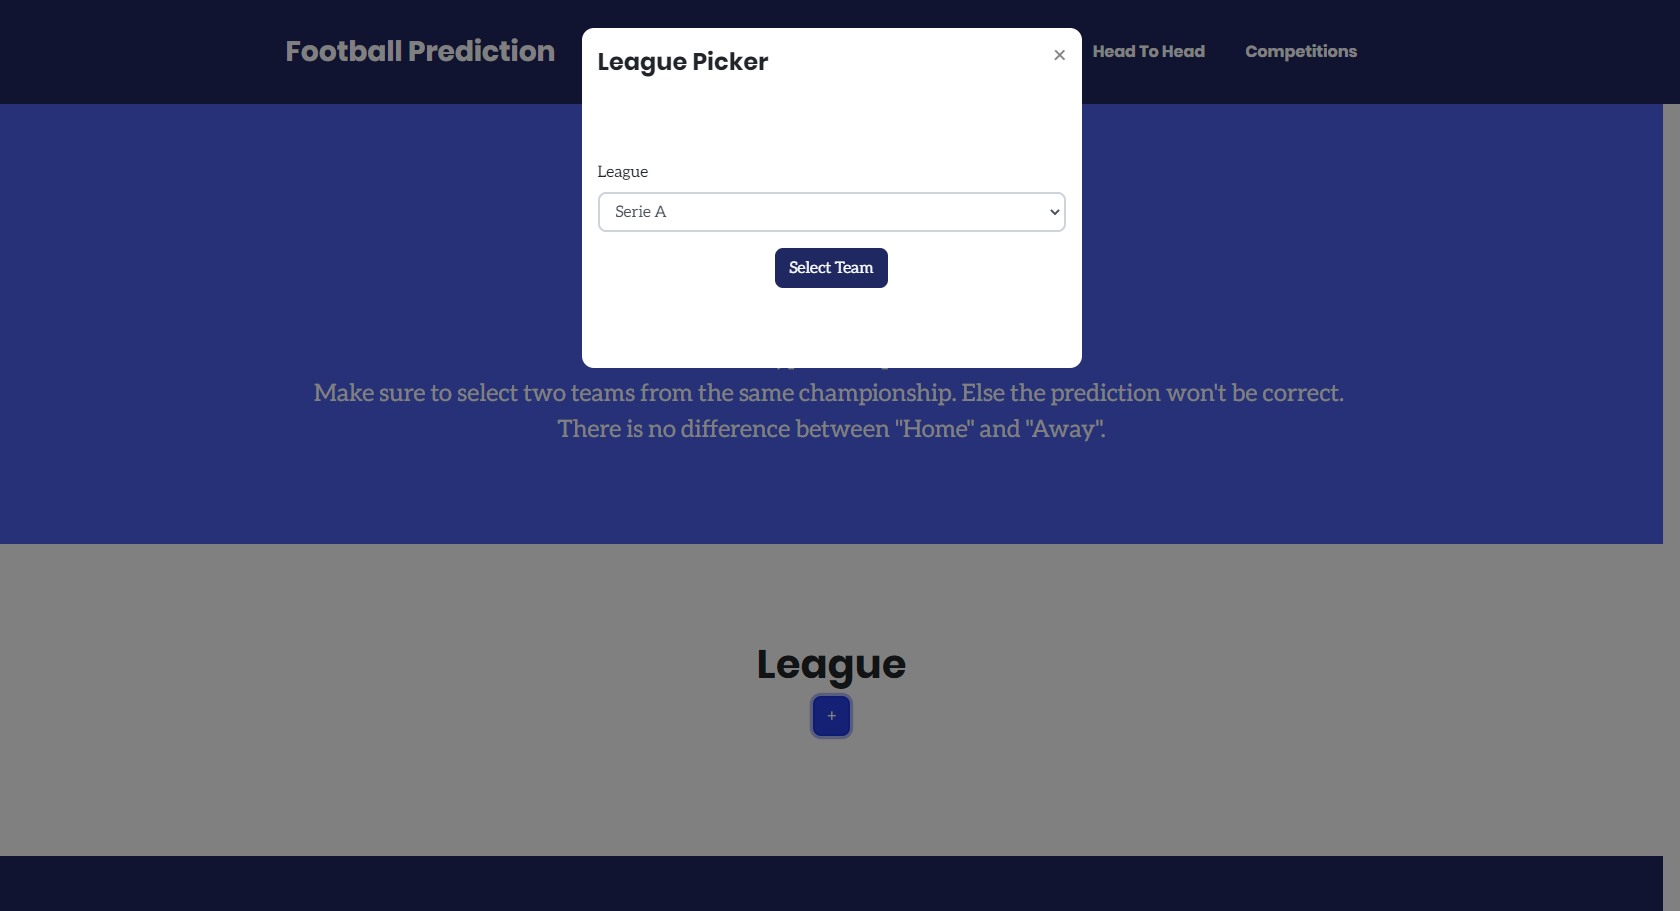
\includegraphics[width=30em]{../img/leaguePickerH2H.png}
    \caption{Aperçu de la page H2H - Sélection de ligue}
    \label{fig:leaguePickerH2H}
\end{figure}

\begin{figure}[htp]
    \centering
    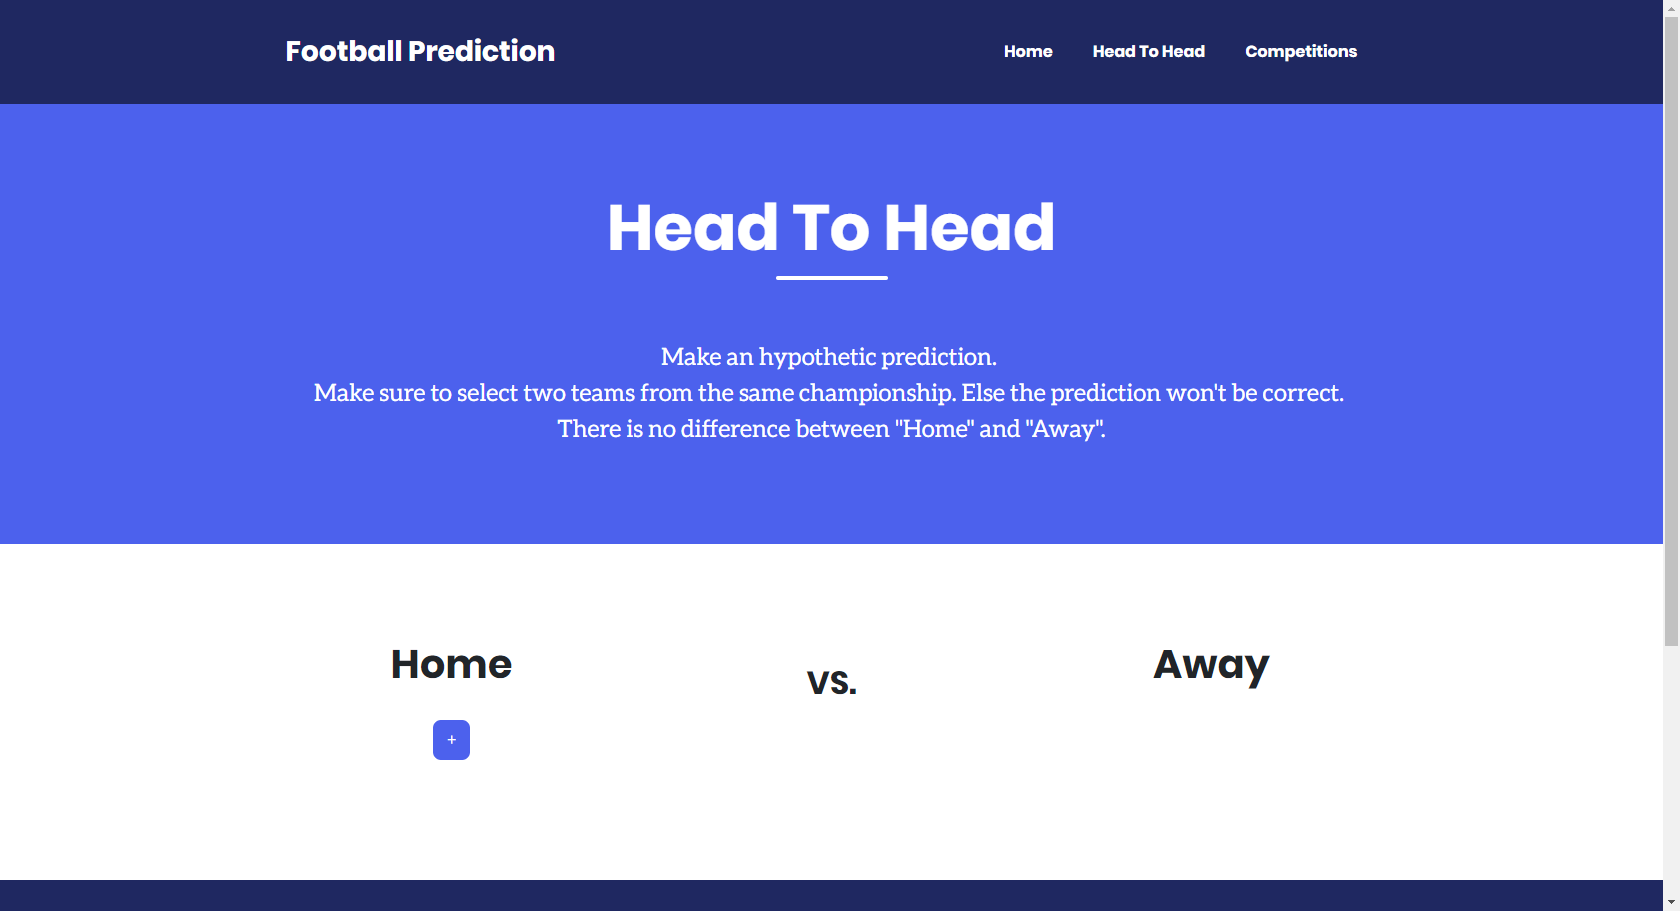
\includegraphics[width=30em]{../img/leagueSelectedH2H.png}
    \caption{Aperçu de la page H2H - Ligue sélectionnée}
    \label{fig:leagueSelectedH2H}
\end{figure}

\begin{figure}[htp]
    \centering
    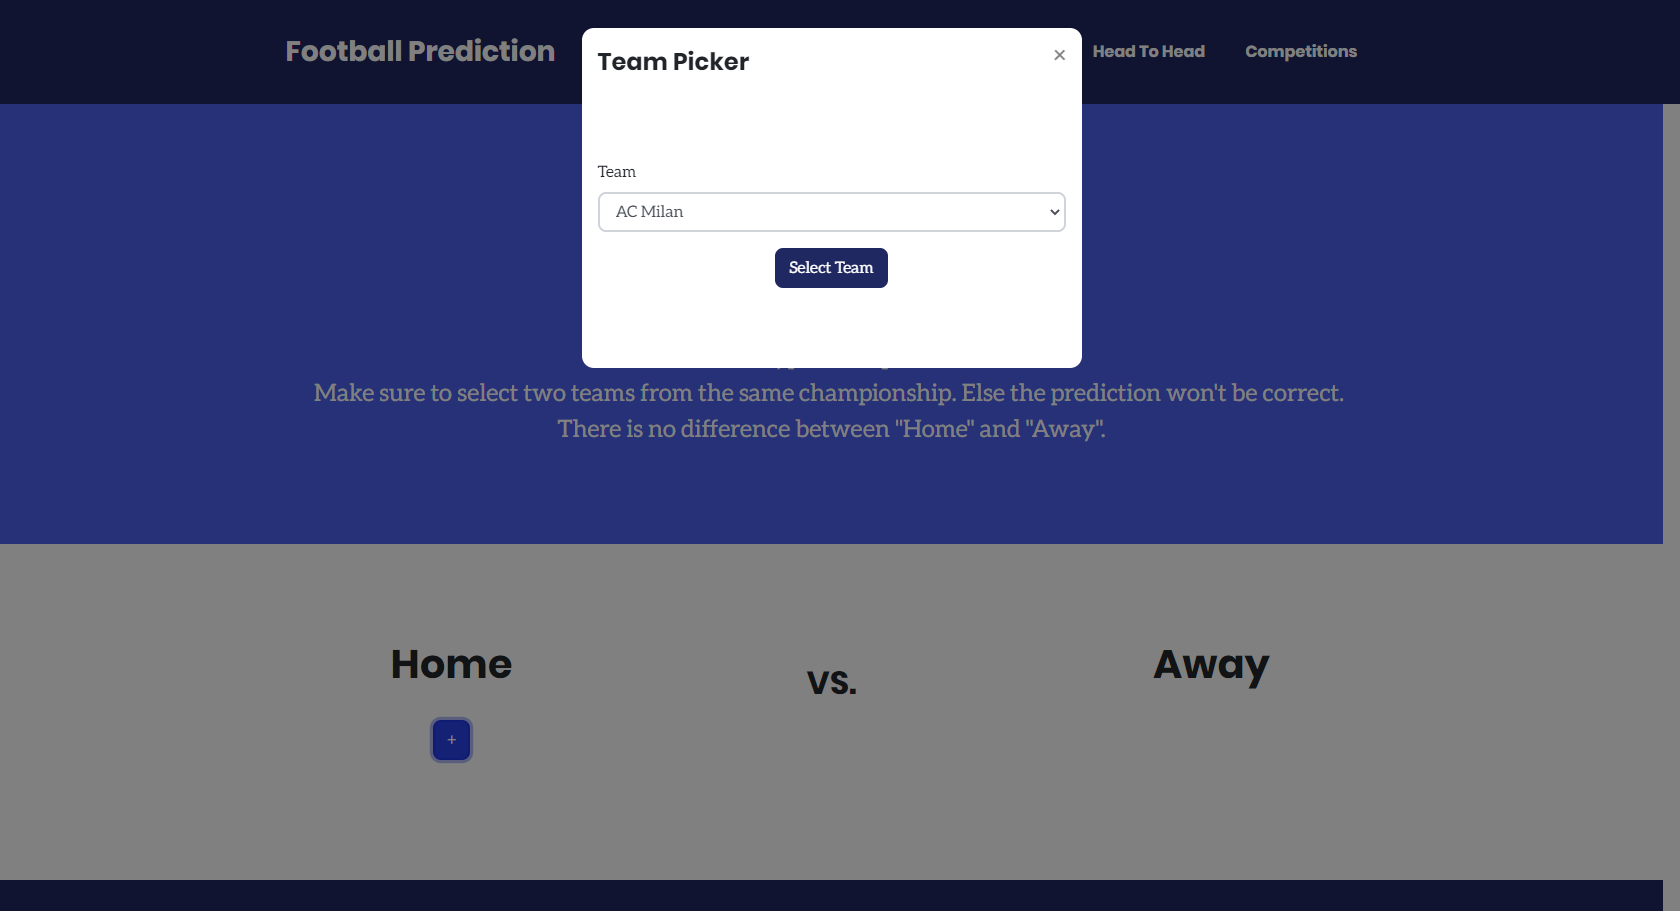
\includegraphics[width=30em]{../img/teamPickerH2H.png}
    \caption{Aperçu de la page H2H - Sélection de l'équipe}
    \label{fig:teamPickerH2H}
\end{figure}

\begin{figure}[htp]
    \centering
    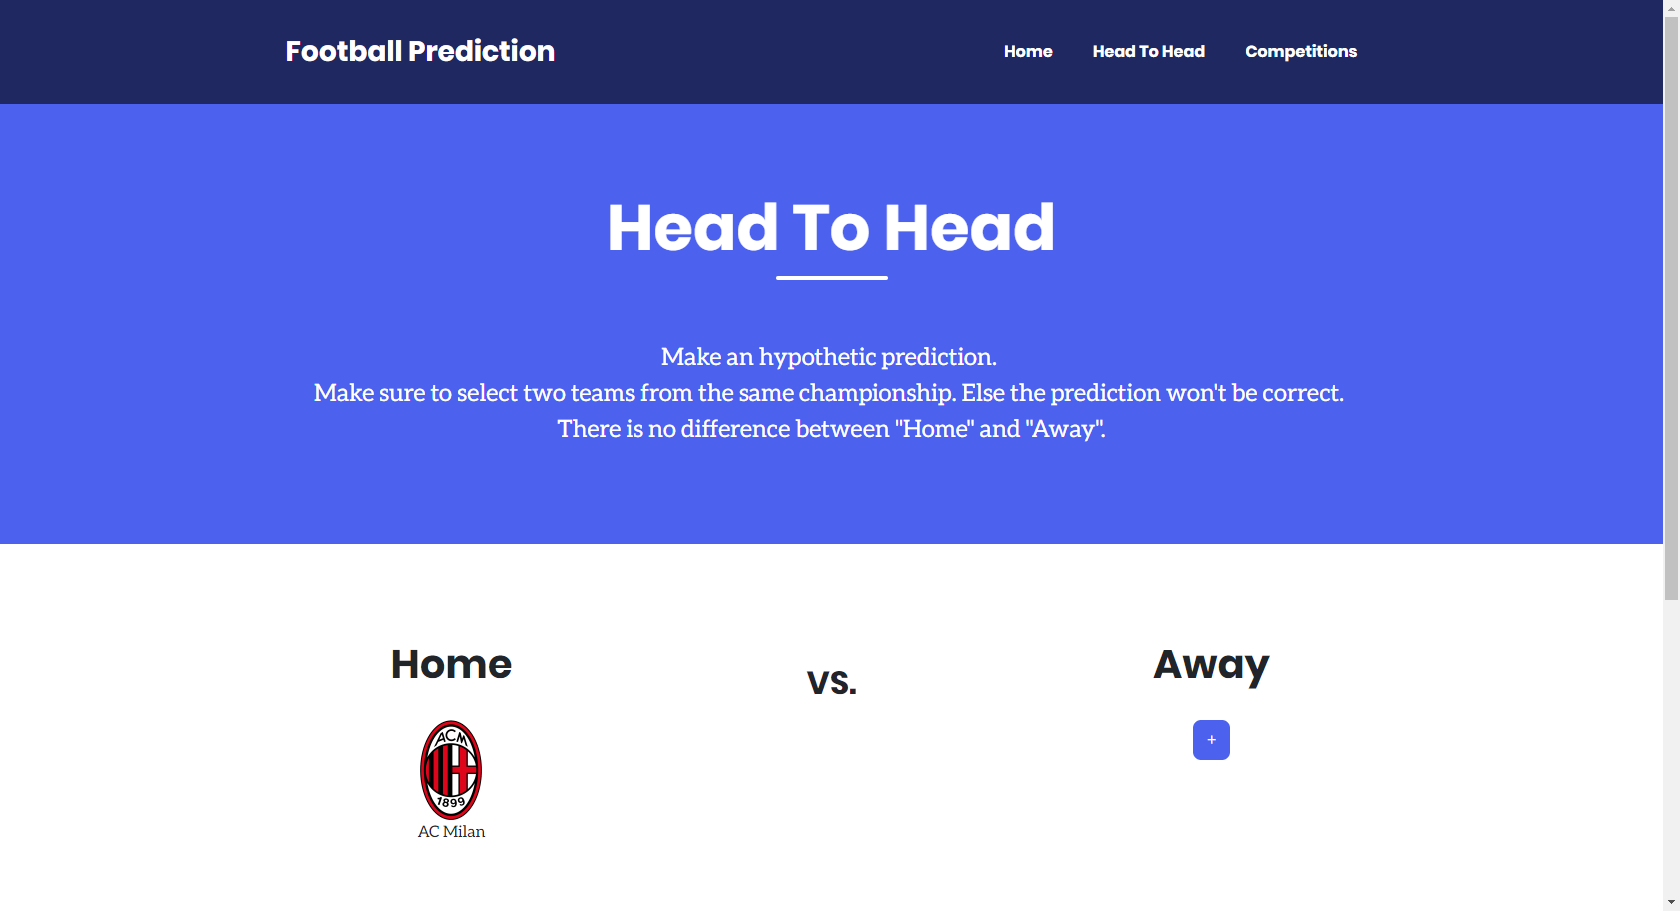
\includegraphics[width=30em]{../img/teamSelectedH2H.png}
    \caption{Aperçu de la page H2H - Première équipe sélectionnée}
    \label{fig:teamSelectedH2H}
\end{figure}

\begin{figure}[htp]
    \centering
    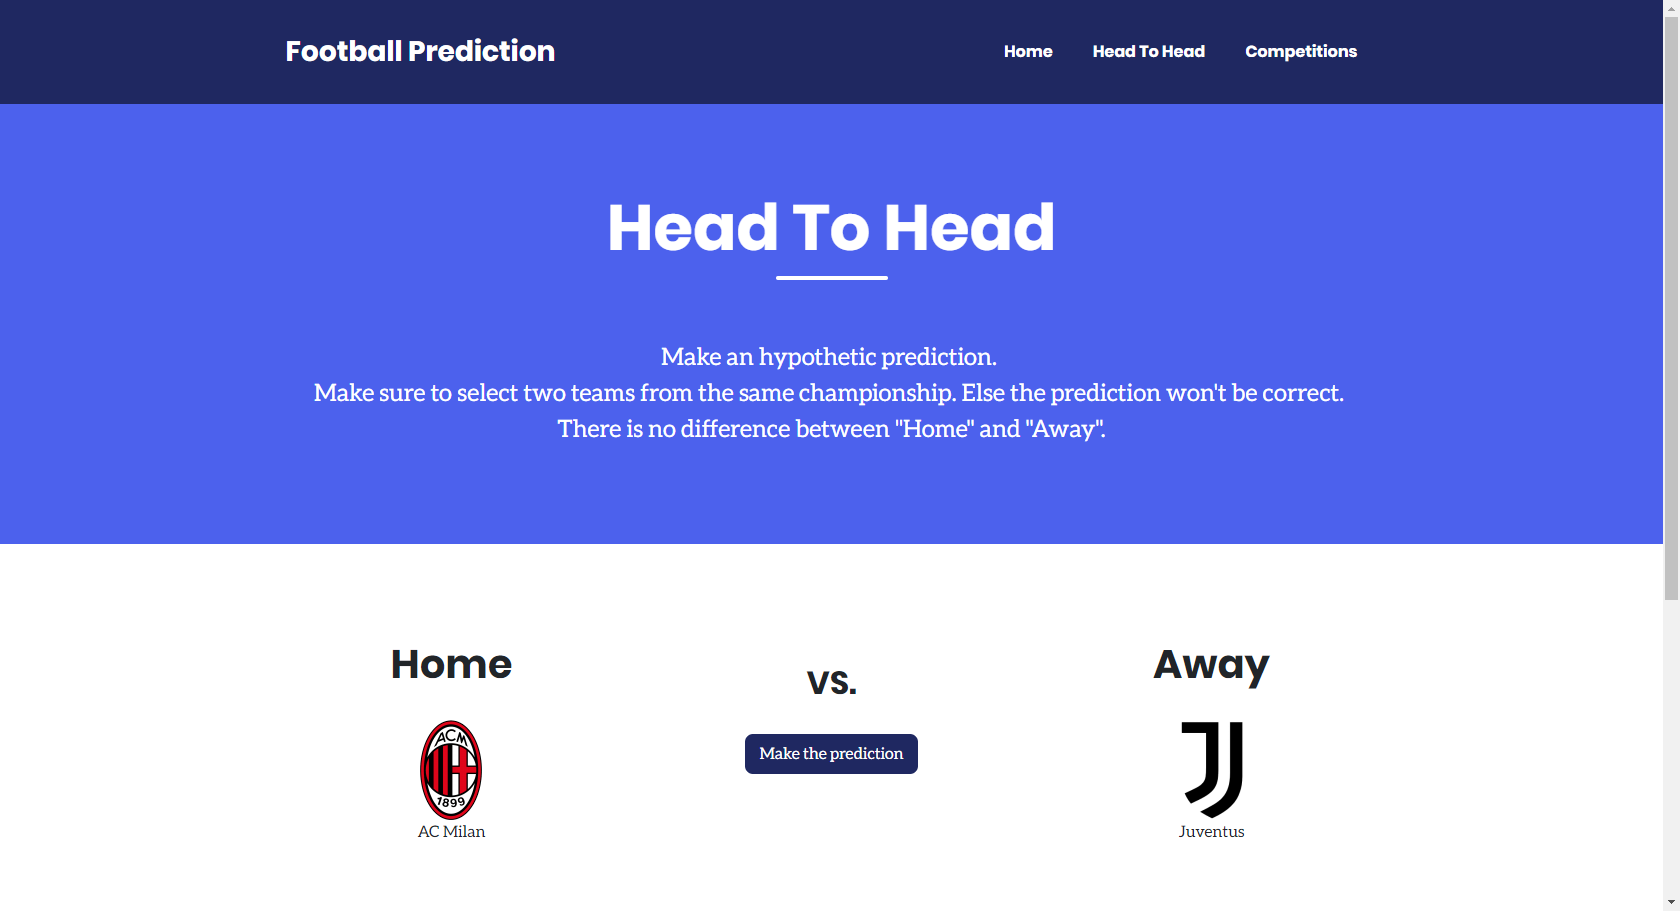
\includegraphics[width=30em]{../img/teamsSelectedH2H.png}
    \caption{Aperçu de la page H2H - Deuxième équipe sélectionnée}
    \label{fig:teamsSelectedH2H}
\end{figure}

\begin{figure}[htp]
    \centering
    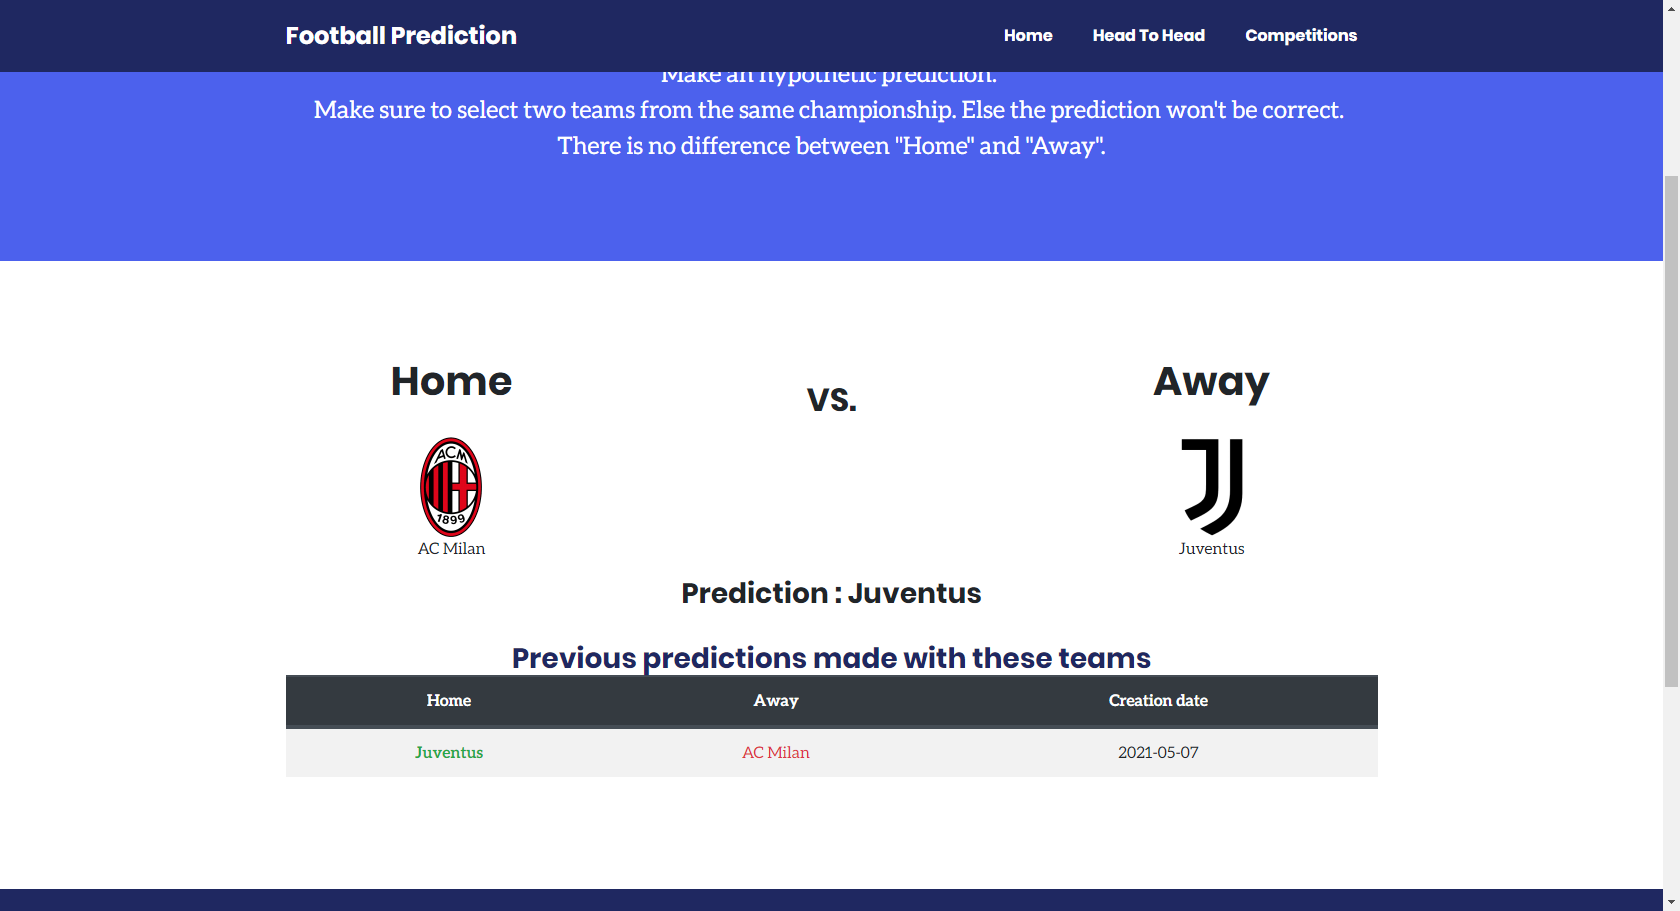
\includegraphics[width=30em]{../img/predictionMadeH2H.png}
    \caption{Aperçu de la page H2H - Prédiction créé}
    \label{fig:predictionMadeH2H}
\end{figure}

\newpage

\subsection{Asynchrone sur la vue}

Dans le point \ref{multiprocessingToAsync}, j'ai expliqué que j'ai du passer sur de l'asynchrone. J'ai donc fait la modification de la vue pour qu'elle puisse utiliser de l'asynchrone. Il y a aucune spécificités liées au fait qu'on utilise Flask.

À noter que l'asynchrone ne fonctionne qu'avec la version 2.X de Python Flask.

\subsection{Competitions}

\subsubsection{Sélection de la ligue}

La sélection de la ligue est la même que la sélection de la ligue pour la fonctionnalité "Head To Head" (voir point \ref{selectionLigueH2H}).

\subsubsection{Création de la prédiction sur toute la compétition}

Pareil que pour la fonctionnalité "Head To Head", j'affiche un gif de loading avec du JS (JQuery) après le choix de la ligue.

Pour ce qui concerne la prédiction sur le championnat, voici comment je m'y suis pris. Tout d'abord, je vérifie que l'ID de la ligue est dans la liste des ligues disponible dans l'application. Si c'est le cas, on crée la compétition et on lance l'élaboration de la prédiction globale puis on récupère le résultat final. Après avoir fait cela, on récupère le contenu de la variable \texttt{missed\_some\_predictions} de \texttt{Competition} qui permet de savoir si tout les matchs ont eu une prédiction (donc qu'il y a eu aucune erreur lors du traitement). Après ça, je récupère une erreur qui est potentiellement stocké dans les cookies (on comprendra dans le point \ref{cookies} la raison). Je l'ai mis dans un \texttt{try except} car la méthode pour récupérer les cookies retourne une Exception si aucun cookie avec la clé spécifiée n'existe. Ensuite, on retourne le template avec le classement, le nombre d'équipes dans le classement, le booléen pour savoir si toutes les prédictions ont été faites et l'erreur. En fin de code, c'est la gestion des erreurs avec l'assignation des valeurs d'erreurs dans les cookies de l'utilisateur.

\lstinputPython{competition-make-prediction}

Pour le code de la vue qui gère l'affichage, on boucle le classement et on affiche les badges, noms, points, victoires, égalités, matchs joués et défaites de chaque équipe. 
\lstinputHTML{competition-make-prediction}

\subsubsection{Historique des matchs}

Pour la route qui permet d'afficher l'historique des matchs d'une équipe dans une compétition, on récupère l'ID de l'équipe sélectionnée, la liste des équipes de la compétition (pour être sûr que l'équipe est bien dans la ligue) et les informations de l'équipe (le nom et le badge). Ensuite, je vérifie que l'équipe soit bien dans la ligue sélectionnée si c'est le cas, on va chercher tout les match de l'équipe choisie et les mettre dans une liste qu'on donnera à la vue. Enfin, on retourne la vue avec les données qu'elle doit afficher
\lstinputPython{competition-history}

Voilà à quoi ressemble le code de la vue qui gère l'affichage des matchs de l'historique.
Je fais une boucle sur le nombre de matchs dans l'historique, j'affiche chaque match et pour chaque match, j'affiche deux puces de couleurs pour déterminer qui est le vainqueur de la prédiction. 
\lstinputHTML{competition-history}

\subsubsection{Aperçus}

\begin{figure}[htp]
    \centering
    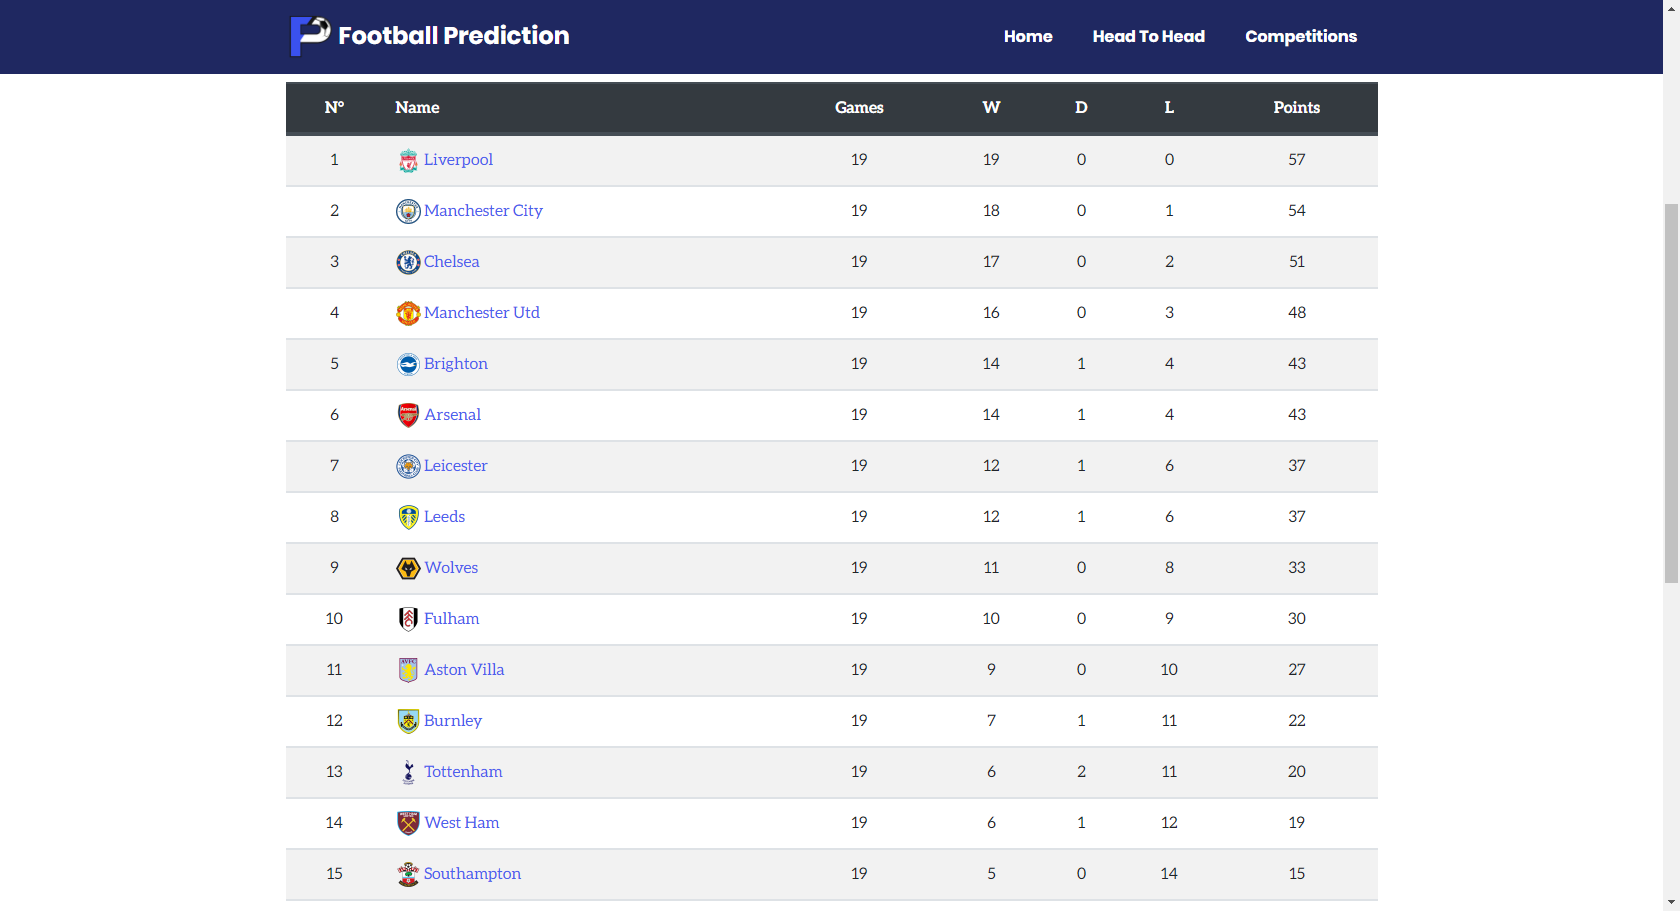
\includegraphics[width=27em]{../img/competitionStanding.png}
    \caption{Aperçu de la page Compétition - Classement affiché}
    \label{fig:competitionStanding}
\end{figure}

\begin{figure}[htp]
    \centering
    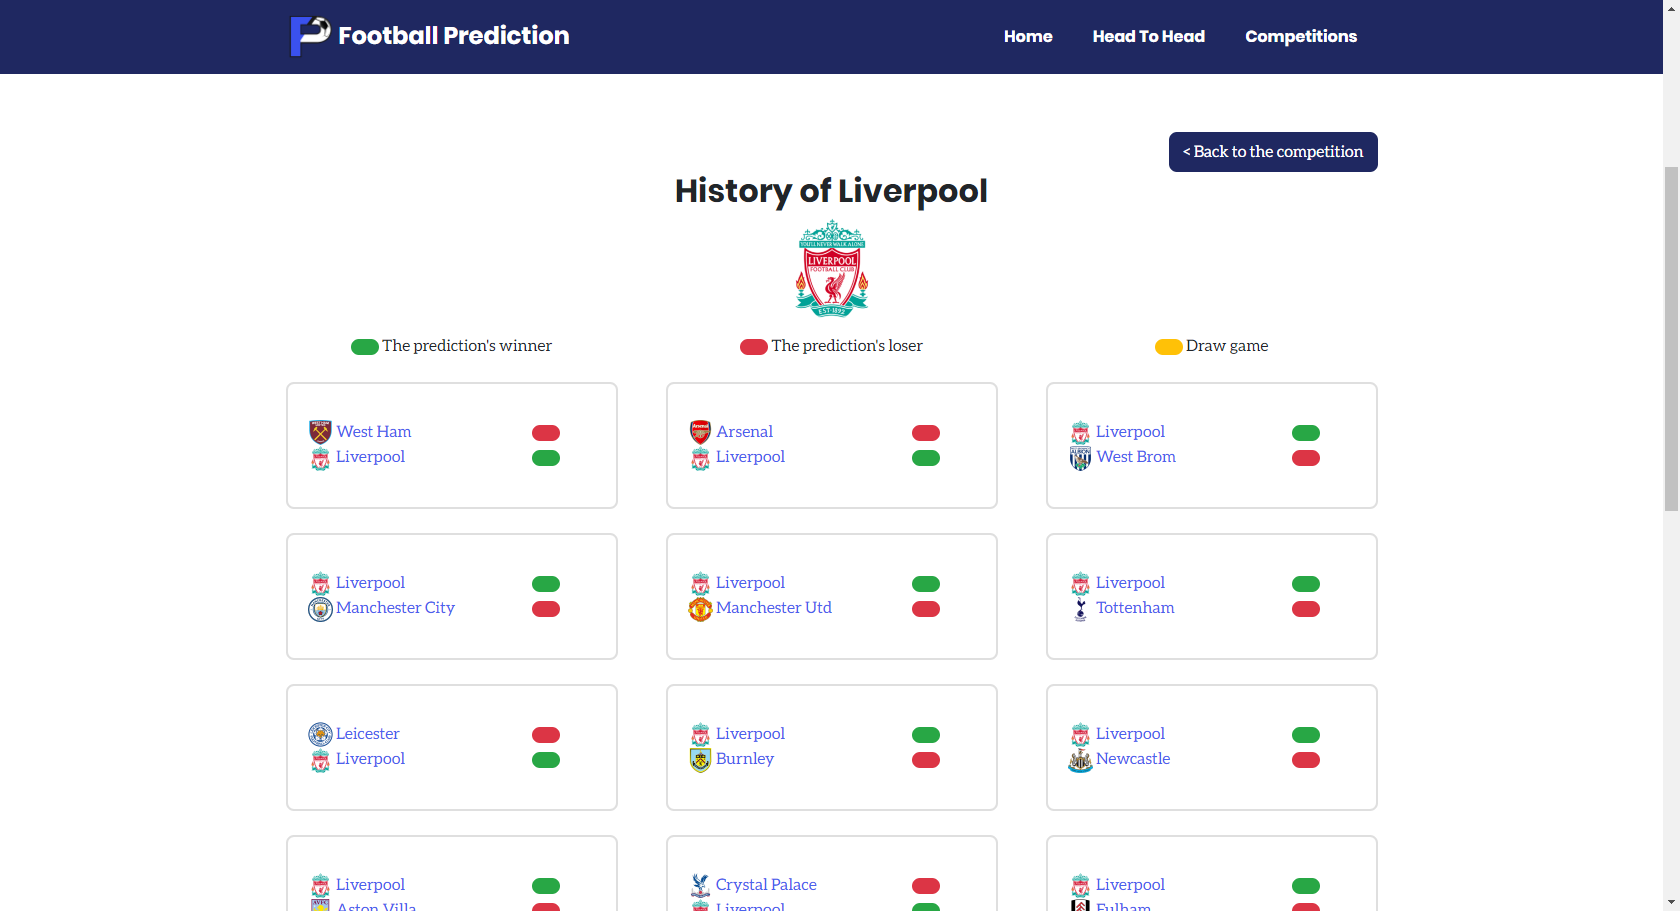
\includegraphics[width=27em]{../img/competitionHistory.png}
    \caption{Aperçu de la page Compétition - Historique d'une équipe}
    \label{fig:competitionHistory}
\end{figure}

\subsection{Cookies}
\label{cookies}

Comme vous pouvez l'apercevoir dans la fonctionnalité "Head To Head" ou encore dans l'accueil , j'avais initialement fait un cache (stocké côté serveur) pour les erreurs venant de l'utilisateur, mais je me suis rendu compte que c'est problématique si plusieurs utilisateurs utilisent le site en simultané. Par exemple, un nouvel utilisateur verrait une erreur en arrivant pour la première fois sur la page H2H, tout ça car un autre utilisateur aurait généré une erreur de son côté.

C'est pourquoi, j'ai décidé d'utiliser les cookies. Ils permettent de stocker des données chez le client. Pour afficher des erreurs qui sont propre à chaque utilisateur, c'est une bien meilleure solution que de les stocker du côté du serveur.

\lstinputPython{cookies-exemple}

Dans le code du listing \ref{list-cookies-exemple}, on doit d'abord créer un objet \texttt{Response}, car c'est cet objet qui nous permet de créer un cookie. Comme paramètre, on donne le lien vers la première page de la fonctionnalité "Head To Head" et on retourne l'objet à \texttt{Response} à la fin. Pour créer un cookie, on appelle la méthode \texttt{set\_cookie}, avec comme premier paramètre la "clé" du cookie, le deuxième est le contenu du cookie et enfin le dernier est son temps de vie en seconde. Ici, son temps de vie est d'une seconde car on l'utilise pour afficher une erreur (L'erreur est affiché qu'une seule fois). 

\lstinputPython{cookies-route}

On peut apercevoir sur la route du listing \ref{list-cookies-route} que cette fois, on fait un \texttt{try except}, car la méthode \texttt{get()} de \texttt{request.cookies} retourne une Exception si la clé n'existe pas. Si on a bien récupéré le cookie, on le transmet à la vue. Autrement, on ne transmet pas l'erreur.

\newpage

\section{Host du site}

Après avoir développé toutes les fonctionnalités, je me suis attelé à l'upload du site sur le serveur de l'école que M. Maréchal m'a mis à disposition pour le travail de diplôme.

Je me suis d'abord connecté au serveur, j'ai cloné mon repository Git et j'ai installer toutes les dépendances contenues dans \texttt{requirements.txt}. J'ai rencontré des soucis lorsque j'ai voulu les installer dans un environnement virtuel mais je me suis dit que cela n'en valait pas la peine puisqu'aucune autre application Python n'allait être sur ce serveur.

J'ai ensuite observé la documentation de Python Flask pour voir les différentes options de déploiement\footnote{\url{https://flask.palletsprojects.com/en/2.0.x/deploying/}}. J'ai du m'orienter sur les options "Self-hosted" puisque le serveur que j'ai à disposition est à l'école. J'ai observé les options et \texttt{mod\_wsgi}\footnote{WSGI est une spécification qui définit l'interface entre les serveurs et les applications webs pour le langage Python.} qui utilise Apache me paraissait être une bonne option. De plus, l'installation me paraissait pas très compliqué. \newline
\texttt{from yourapplication import app as application}

Et ensuite, j'ai du configurer Apache pour qu'il comprenne en indiquant les commandes \texttt{WSGI*} que c'est une application Flask. J'avais bien fait attention de tester avec une application Flask lambda (qu'une seule route voir si le retour était bon) et elle fonctionnait correctement. Cependant, lorsque j'ai ajouté mon application, les importations de modules avaient du mal à se faire. C'était initialement des problèmes venant des permissions sur les fichiers mais j'ai ensuite donné la propriété des fichiers à l'utilisateur et au groupe \texttt{www-data}. Mais, après avoir fait cela, il n'arrivait pas à importer les sous-paquets contenus dans \texttt{lib}. J'ai essayé de changer la manière d'importer les modules de beaucoup de façons mais j'ai finalement pris une autre option, car le délai était avant la réddition du travail.

Je me suis donc tourné vers Gunicorn\footnote{\url{https://flask.palletsprojects.com/en/2.0.x/deploying/wsgi-standalone/}} qui est un paquet Python WSGI HTTP fait pour Unix. Son installation et sa mise en place m'ont paru parfait pour le temps que j'avais à disposition. Cependant, j'ai tout de même eu du mal initialement, puisqu'il fallait ouvrir les ports du serveur. Grâce à l'aide de M. Garcia, le problème a été résolu et on a enfin eu accès à l'application web.

L'application est donc disponible à l'adresse suivante (accessible uniquement dans le réseau du CFPT) : \newline \url{http://soccer-pronostic.cfpt.info:8080/} 

La documentation est disponible à l'adresse suivante (accessible uniquement dans le réseau du CFPT) : \newline \url{http://soccer-pronostic.cfpt.info/doc} 

\newpage

\section{Tests}

\subsection{Tests des méthodes du code}

J'ai créé différents scripts qui testent les méthodes de chacune des classes. Ces scripts servent à vérifier que le format des données retournées par les méthodes est bon et que les méthodes asynchrones sont efficaces.

\lstinputPython{test-provider}

Ici, je veux tester que la méthode \texttt{get\_all\_stats\_from\_teams()} retourne bien les données dans le bon format. Cette dernière est asynchrone, c'est pourquoi je la mets dans une méthode async car le mot clé \texttt{await} ne peut pas être utilisé s'il n'est pas dans une méthode \texttt{async}. Autrement, j'aurais pu mettre la méthode directement dans le \texttt{asyncio.run()} mais ce n'est pas possible si je souhaite appeler plusieurs méthodes asynchrones à la suite.
Tous les autres tests des méthodes font globalement la même chose (test sur le format du retour de la méthode).

\subsection{Tests sur la vue}

Comme indiqué dans le point \ref{outilAutomatisationTest}, j'ai utilisé Katalon Recorder pour tester ma vue.

\begin{figure}[htp]
    \centering
    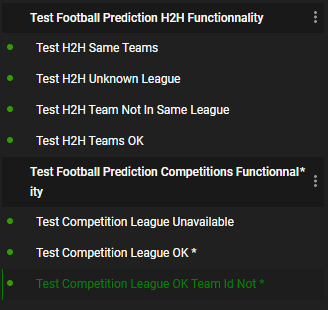
\includegraphics[width=15em]{../img/katalonTestsSurVue.png}
    \caption{Liste des tests sur la vue}
    \label{fig:predictionMadeH2H}
\end{figure}

On peut apercevoir que je n'ai pas testé l'accueil de la vue. En effet, la vue ne nécessite aucune manipulation de la part de l'utilisateur, donc il n'y aucun risque vis-à-vis d'une mauvaise intention ou manipulation de l'utilisateur.

J'ai donc testé uniquement la fonctionnalité "Head To Head" et la fonctionnalité "Competitions". 

\newpage

\subsubsection{Test H2H : Même équipes}

\begin{table}[htp]
    \centering
    \begin{tabular}{|m{4cm}|m{4cm}|m{6cm}|}
    \hline
    \textbf{Commande} & \textbf{Valeur}                                      & \textbf{Description}                                                                    \\ \hline
    open              &                                                      & Ouverture de la route "Head To Head"                                           \\ \hline
    click             &                                                      & Ouverture de la fenêtre modale de la ligue                                              \\ \hline
    click             &                                                      & Sélection de la ligue (par défaut : "Premier League")                                   \\ \hline
    click             &                                                      & Ouverture de la première fenêtre modale d'équipe                                        \\ \hline
    click             &                                                      & Sélection de la première équipe (par défaut : "Arsenal")                                \\ \hline
    assertText        & Arsenal                                              & Vérification que le texte "Arsenal" apparaisse sur la vue                               \\ \hline
    click             &                                                      & Ouverture de la deuxième modal d'équipe                                                 \\ \hline
    click             &                                                      & Sélection de la deuxième équipe (par défaut : "Arsenal")                                \\ \hline
    assertText        & Arsenal                                              & Vérification que le texte "Arsenal" apparaisse sur la vue                               \\ \hline
    click             &                                                      & Validation du choix des équipes                                                         \\ \hline
    assertTextPresent & You cannot pick the same teams to make a prediction. & On vérifie que l'erreur apparaisse bien sur la vue                                      \\ \hline
    assertVisible     &                                                      & On vérifie qu'on ait le bouton pour choisir la ligue. (Retour à la page H2H principale) \\ \hline
    \end{tabular}
    \label{tab:H2HMemeEquipes}
    \caption{H2H - Erreur même équipe sélectionnée}
\end{table}

\newpage

\subsubsection{Test H2H : Ligue inconnue}

\begin{table}[htp]
    \centering
    \begin{tabular}{|m{4cm}|m{4cm}|m{6cm}|}
    \hline
    \textbf{Commande} & \textbf{Valeur} & \textbf{Description}                                                                                                                              \\ \hline
    open              &                 & Injection d'un mauvais ID de ligue dans l'url \\ \hline
    assertTextPresent & Unknown league. & Vérification que l'erreur apparaisse sur la vue                                                                                                   \\ \hline
    assertVisible     &                 & On vérifie qu'on ait le bouton pour choisir la ligue. (Retour à la page H2H principale)                                                           \\ \hline
    \end{tabular}
    \label{tab:H2HLigueInconnue}
    \caption{H2H - Ligue inconnue}
\end{table}

\subsubsection{Test H2H : Équipes pas dans la ligue sélectionnée}

\begin{table}[htp]
    \centering
    \begin{tabular}{|m{4cm}|m{4cm}|m{6cm}|}
    \hline
    \textbf{Commande} & \textbf{Valeur} & \textbf{Description}                                                                                                                              \\ \hline
    open              &                 & Injection d'un mauvais ID d'équipe dans l'url \\ \hline
    click             &                 & Validation du choix des deux équipes                                                                                                   \\ \hline
    assertTextPresent & Teams not found in this league. & On vérifie que l'erreur apparaisse bien sur la vue.                                                           \\ \hline
    assertVisible     &                 & On vérifie qu'on ait le bouton pour choisir la ligue. (Retour à la page H2H principale)                                                           \\ \hline
    \end{tabular}
    \label{tab:H2HEquipePasDansLigue}
    \caption{H2H - Équipes pas dans la ligue sélectionnée}
\end{table}

\newpage

\subsubsection{Test H2H : Succès}

\begin{table}[htp]
    \centering
    \begin{tabular}{|m{4cm}|m{4cm}|m{6cm}|}
    \hline
    \textbf{Commande} & \textbf{Valeur}                                      & \textbf{Description}                                                                    \\ \hline
    open              &                 & Ouverture de la route "Head To Head"                                          \\ \hline
    click             &                 & Ouverture de la fenêtre modale de la sélection de ligue                       \\ \hline
    select            & label=Serie A   & Sélection de la "Serie A" comme ligue                                         \\ \hline
    click             &                 & Validation                                                                    \\ \hline
    select            & label=Napoli    & Sélection de "Napoli"                                                         \\ \hline
    click             &                 & Validation                                                                    \\ \hline
    assertText        & Napoli          & Vérification que "Napoli" apparaisse sur la vue                               \\ \hline
    select            & label=AS Roma   & Sélection de "AS Roma"                                                        \\ \hline
    click             &                 & Validation                                                                    \\ \hline
    assertText        & AS Roma         & Vérification que "AS Roma" apparaisse sur la vue                              \\ \hline
    click             &                 & Validation de la prédiction.                                                  \\ \hline
    assertTextPresent & Prediction :    & Vérification que le résultat de la prédiction soit retourné par l'application \\ \hline
    assertNotVisible  &                 & On s'assure que le bouton pour choisir la ligue soit pas visible              \\ \hline
    \end{tabular}
    \label{tab:H2HSucces}
    \caption{H2H - Succès}
\end{table}

\newpage

\subsubsection{Test Competition : Ligue inconnue}

\begin{table}[htp]
    \centering
    \begin{tabular}{|m{4cm}|m{4cm}|m{6cm}|}
    \hline
    \textbf{Commande} & \textbf{Valeur}                                      & \textbf{Description}                                                                    \\ \hline
    open              &                 & Injection d'un ID de ligue invalide depuis l'url \\ \hline
    assertTextPresent & Unknown league. & Vérification que l'erreur apparaisse sur la vue                                                                                                   \\ \hline
    assertVisible     &                 & On vérifie qu'on ait le bouton pour choisir la ligue. (Retour à la page Competitions principale)     \\ \hline
    \end{tabular}
    \label{tab:CompLigueInconnue}
    \caption{Competition - Ligue inconnue}
\end{table}

\subsubsection{Test Competition : Identifiant de l'équipe incorrect}

\begin{table}[htp]
    \centering
    \begin{tabular}{|m{4cm}|m{4cm}|m{6cm}|}
    \hline
    \textbf{Commande} & \textbf{Valeur} & \textbf{Description} \\ \hline
    open              &                 & Ouverture de la route "Competitions" \\ \hline
    click             &                 & Ouverture de la fenêtre modale pour la sélection de ligue \\ \hline
    click             &                 & Validation du choix de la ligue (par défaut : "Premier League") \\ \hline
    open              &                 & Injection d'un ID invalide depuis l'url   \\ \hline
    assertTextPresent & N*              & Vérification que le tableau soit affiché ("N*" est le nom d'une colonne dans le classement de la compétition)     \\ \hline
    assertTextPresent & This team is not in the league. & Vérification que l'erreur apparaisse bien sur la vue.     \\ \hline
    \end{tabular}
    \label{tab:CompIdIncorrect}
    \caption{Competition - ID d'équipe incorrect pour l'historique des matchs}
\end{table}

\newpage

\subsubsection{Test Competition : Succès}

\begin{table}[htp]
    \centering
    \begin{tabular}{|m{4cm}|m{4cm}|m{6cm}|}
    \hline
    \textbf{Commande} & \textbf{Valeur}            & \textbf{Description}                                                                                          \\ \hline
    open              &                            & Ouverture de la route "Competitions"                                                                          \\ \hline
    click             &                            & Ouverture de la fenêtre modale pour la sélection de ligue                                                     \\ \hline
    select            & label=Premier League       & Choix de la ligue "Premier League"                                                                            \\ \hline
    click             &                            & Validation                                                                                                    \\ \hline
    assertTextPresent & N*                         & Vérification que le tableau soit affiché ("N*" est le nom d'une colonne dans le classement de la compétition) \\ \hline
    assertNotVisible  &                            & Vérification que le bouton qui affiche la fenêtre modale de sélection de ligue ait disparu.                   \\ \hline
    click             &                            & Clic sur "Manchester City" afin d'avoir accès à l'historique de l'équipe.                                     \\ \hline
    assertTextPresent & History of Manchester City & On s'assure qu'on arrive sur la page de l'historique de l'équipe choisie auparavant.                          \\ \hline
    \end{tabular}
    \label{tab:CompSucces}
    \caption{Competition - Succès}
\end{table}

\newpage

\section{Pré-mise en production}

Avant de mettre le projet en production, il faut \texttt{absolument} rédiger des conditions générales d'utilisation. En effet, les CGU permettrait de protéger mes données ainsi que de me protéger du fait que les prédictions fournies par l'application ne sont pas une véritié absolue. Cela me protègerait si un utilisateur irait misé et qu'il aimerait se retourner contre moi pour X ou Y raisons. S'il viendrait se plaindre, je l'inviterais à lire les conditions générales d'utilisation.

\newpage

\section{Retour d'expérience}

\subsection{Points positifs}

Globalement, j'ai pu ressortir pas mal de points positifs concernant ce travail de diplôme. Tout d'abord, le fait de travailler sur un projet aussi conséquent et de cette ampleur. C'est une expérience que j'ai très rarement fait dans toute ma formation et j'en ressors toujours du positif.

Ensuite, l'apprentissage de nouvelles technologies est quelque chose de positif. Cela m'a appris à comprendre de nouveaux principes de programmation (multiprocessing, asynchrone). 

Enfin, je ressors de positif une pratique que j'ai rarement effectué et que j'ai expérimenté réellement durant tout mon travail. Le fait de poser mes réflexions sur une feuille et de schématiser le fonctionnement des algorithmes sur une feuille. Cela a peut-être l'air d'être insignifiant mais j'ai vraiment ressenti un gain de productivité grâce à ça. Généralement, je commençais directement à coder mais ici, ça m'a permis de trouver plein de problèmes avant l'implémentation de certains algorithmes.

\subsection{Problèmes rencontrés}

\subsubsection{Multiprocessing}
Ce point va sûrement se répéter avec le point \ref{multiprocessingToAsync}.

Le problème que j'ai rencontré avec le multiprocessing était que les Process se bloquaient pour une raison inconnue que je n'ai pas réussi à trouver. Ce problème a été rencontré lors du développement de la classe \texttt{Competition}. Débugger un code qui utilise du multiprocessing est très complexe et je n'ai malheureusement pas trouvé la source du problème. Cependant, j'ai tout de même trouvé une solution. En effet, après avoir posé mon problème sur un forum communautaire, j'ai reçu des réponses rapides et pertinentes. Et la majorité des réponses me conseillait d'utiliser de l'asynchrone plutôt que du multiprocessing, car c'était beaucoup plus adapté à mon travail. Pour rappel, j'avais choisi de faire du multiprocessing, car si je voulais passer sur de l'asynchrone initialement, j'aurais du changer une bonne partie de mon code (au final, j'ai du le faire quand même).

Après être passé sur de l'asynchrone et avoir changé mes méthodes de bas et de haut niveaux, je n'ai plus eu de problèmes.

\subsubsection{Fréquence d'appel à l'API trop élevée}
Ce problème a été présent lors de l'asynchrone et aussi du multiprocessing. Pour être au clair, pour prédire une compétition, des appels à l'API sont fait pour récupérer les résultats des derniers matchs de chacune des équipes. Cependant, la quantité d'appels qui sont faits était très élevée. Cela avait pour conséquence de rendre le serveur de l'API que j'utilise très lent et il arrivait parfois qu'il retourne des erreurs \texttt{500}. J'ai tout de même réussi à "résoudre" ce soucis en faisant un cache sur les appels faits dans la journée pour réduire le nombre d'appels fait à l'API de manière considérable. Cependant, le soucis va tout de même apparaître la première fois que l'on prédit une compétition dans la journée.

\subsection{Zone grise}

\subsubsection{Planification}

La planification dans ce projet a été dans une "zone grise"\footnote{J'entends par "zone grise" le fait que ça ait été un point faible mais que j'en ai pas réellement souffert.}. Il y a eu un manque de planification dans mon projet. Je n'avais pas réellement idée du temps que j'allais prendre pour produire la classe \texttt{Prediction}, la classe \texttt{Competition} ou encore pour produire la vue. De plus, je ne me suis pas remis en question sur l'importance et la priorité des fonctionnalités.

Tout cela aurait pu m'être très problématique si j'avais rencontré des points bloquants lors de mon travail. Cependant, je spécifie, je mets la planification dans le point "zone grise" car cela ne m'a pas porté préjudice.

\subsubsection{Tests}

Une autre zone grise sont les tests (plus particulièrement, les tests du "backend"). Effectivement, il aurait été plus judicieux de tester unitairement les méthodes du backend (par exemple la classe \texttt{Prediction}). Je n'ai pas fait d'analyse complète sur toutes mes méthodes pour savoir lesquelles est-ce que je devrais tester. J'aurais du tester unitairement les méthodes des classes en faisant des Mocks\footnote{Le but d'un Mock est d'hériter d'une classe dépendante à la classe que l'on veut tester. Le Mock sert ensuite à s'assurer que les données restent systématiquement les mêmes et on teste l'intéraction avec la classe et non les données.} mais j'ai négligé les tests du "backend" et je suis resté sur un test sur le bon format de retour des méthodes.

Comme pour la planification, la manque de tests du backend aurait pu me porter préjudice, mais j'ai tout de même tester le frontend qui interagit avec le backend, ce qui me permet tout de même de d'avoir des tests unitaires.

\subsection{Résultat}

Malgré les problèmes rencontrés, j'ai tout de même réussi à produire l'ensemble du travail visé. Le cahier des charges a été respecté et les fonctionnalités demandées sont présents. L'interface web a été faite et elle communique avec le backend grâce à Python Flask.

\subsection{Améliorations futures}
Comme améliorations futures, je souhaiterais premièrement ajouter un graphique "radar" dans la fonctionnalité "Head To Head". Cette amélioration m'a été inspiré par Pro Evolution Soccer. L'ajout de ce graphique permettrait à l'utilisateur de montrer à quelle point l'équipe qui a été prédit vainqueur est devant son adversaire (voir fig. \ref{fig:graphRadar}).

\begin{figure}[htp]
    \centering
    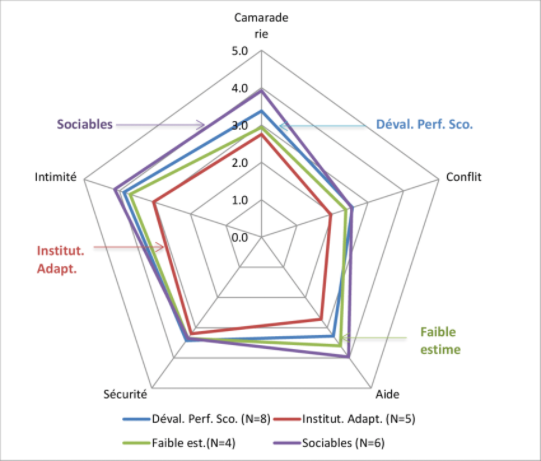
\includegraphics[width=20em]{../img/graphRadar.png}
    \caption{Graphique Radar}
    \label{fig:graphRadar}
\end{figure}

Ensuite, une autre amélioration serait de perfectionner l'élaboration des prédictions. Pour l'instant, l'élaboration des prédictions se fait via les statistiques des derniers matchs et ne prend pas en compte les matchs à domicile ou l'importance du match. L'amélioration serait de permettre de choisir l'importance du match et de prendre en compte le fait que le match est joué à domicile ou non.

La troisième amélioration serait de faire un compteur pour montrer le pourcentage de réussite de l'application. L'utilisateur viendrait sur la page d'accueil et il aurait un aperçu de la fiabilité de l'application. 

La dernier amélioration serait de passer à la version 3.0 de l'API. Cependant, cela nécessiterait une nouvelle analyse sur l'importance des statistiques et un changement dans le code de la classe \texttt{Prediction} et du \texttt{Provider}

\subsection{Bilan personnel}
Je suis satisfait du travail rendu après ces 9 semaines. Un travail de cet ampleur implique forcément des problèmes surtout à la rencontre de nouvelles technologies. J'ai eu des soucis avec le multiprocessing mais ça ne m'a pas empêché de finir la fonctionnalité \texttt{Competition}. J'ai pu prendre en main de nouvelles technologies comme Python Flask, l'asynchrone en Python ou encore le multiprocessing. 

\newpage

\subsection{Apports personnels}

Le tableau ci-dessous présente mon apport personnel dans ce projet. 

\begin{table}[htp]
    \centering
    \begin{tabular}{|m{4cm}|m{4cm}|m{6cm}|}
    \hline
    \textbf{Nom}                                    & \textbf{Pourcentage} & \textbf{Commentaire}                                                                                                    \\ \hline
        Style du site                                   & 5\%                  & Le style provient d'un template Bootstrap                                                                               \\ \hline
        Interface Web                                   & 95\%                 &                                                                                                                         \\ \hline
        Base de données                                 & 100\%                &                                                                                                                         \\ \hline
        Poster                                          & 50\%                 & Gawen Ackermann m'a aidé pour faire le poster                                                                           \\ \hline
        Documentation                                   & 100\%                &                                                                                                                         \\ \hline
        Maquettes                                       & 100\%                &                                                                                                                         \\ \hline
        Requêtes SQL                                    & 95\%                 & M. Schmid m'a aidé sur une requête sur laquelle j'avais de la difficulté                                                \\ \hline
        Communication avec l'API                        & 75\%                 & J'ai utilisé la librairie aiohttp (requests au départ) pour faire les appels HTTP à l'API.                              \\ \hline
        Élaboration des prédictions et des compétitions & 99.9\%               & M. Schmid m'a aidé lors de mes réflexions. Cela m'a permis d'avoir un point de vue différent lors de certaines analyses \\ \hline
    \end{tabular}
    \caption{Apports personnels}
    \label{tab:apportsPersonnels}
\end{table}

\newpage

\section{Conclusion}

Lors de ces 9 semaines de travail, j'ai pu créer une application web qui permet de visualiser les résultats de prédictions sur des matchs de football\footnote{Prédiction que j'ai élaboré moi-même}, en utilisant des technologies avec lesquelles je n'avais aucune expérience auparavant, comme Python Flask, le multiprocessing, etc.

Je reconnais avoir fait une erreur quand au départ j'ai directement démarré le projet en faisant des appels synchrones à l'API. Ce choix a eu un impact sur la suite de mon travail puisqu'il m'a bloqué lors de la conception de la classe de \texttt{Competition}. J'ai du modifier mon code pour qu'il fonctionne avec des appels asynchrones pour permettre à cette classe de fonctionner comme prévu.

Ce projet de grande envergure m'a appris l'importance de prendre du temps pour analyser les fonctionnalités voulues et schématiser leur fonctionnement pour faciliter l'implémentation. Il m'a aussi permis de me rendre compte de l'importance de la planification et de l'importance de l'analyse complète de technologies existantes pour la conception de fonctionnalités

\subsection{Remerciements}

Mes remerciements à :
\begin{itemize}
    \item Antoine Schmid pour son aide, ses conseils, sa réactivité aux communications et son suivi tout au long du projet.
    \item Francisco Garcia pour ses conseils
    \item L'équipe de développeurs d'APIFootball pour l'élevation de plan offerte durant la période du diplôme
    \item Jonathan Borel-Jaquet, Fabian Huber, Lorenzo Bauduccio et Gawen Ackermann pour avoir apporter leur avis lors de certaines réflexions
    \item Gawen Ackermann pour l'aide lors de la réalisation du poster.
    \item Le Discord Not A Name
\end{itemize}

\newpage

\section{Bibliographie}

\textbf{Information à propos des listings} 

Dans le rapport, les listings sont des bouts de codes et les noms de fichiers ne sont pas les mêmes que dans le projet. Tout ceci a été fait pour simplifier la lecture du rapport.

\setlength{\parskip}{0em}

\listoffigures

\lstlistoflistings

\listoftables

\end{document}
